% CREATED BY DAVID FRISK, 2016
% MODIFIED BY JAKOB JARMAR, 2016
% A few changes by Birgit Grohe, 2017 and 2018
% Adjustments with the help of Gustav Örtenberg 2019
% Parskip % bibliography system updated by Erik Ljungdahl, May 2022

% IMPORT SETTINGS
\documentclass[12pt,a4paper,twoside,openright]{report}
% \listfiles % To be able to reproduce on other machines
% CREATED BY DAVID FRISK, 2016

% BASIC SETTINGS
\usepackage{moreverb}								% List settings
\usepackage{textcomp}								% Fonts, symbols etc.
\usepackage{lmodern}								% Latin modern font
\usepackage{helvet}									% Enables font switching
\usepackage[T1]{fontenc}							% Output settings
\usepackage[english]{babel}							% Language settings
\usepackage[utf8]{inputenc}							% Input settings
\usepackage{amsmath}								% Mathematical expressions (American mathematical society)
\usepackage{amssymb}								% Mathematical symbols (American mathematical society)
\usepackage[pdf]{graphviz}                          % dot-files directly in latex
\usepackage{graphicx}								% Figures
% \usepackage{subfig}									% Enables subfigures
\usepackage{caption}
\usepackage{subcaption}
\usepackage{acronym}                                % For a list of abbreviations
\usepackage{glossaries}
\usepackage{tikz-dependency}

\numberwithin{equation}{chapter}					% Numbering order for equations
\numberwithin{figure}{chapter}						% Numbering order for figures
\numberwithin{table}{chapter}						% Numbering order for tables
\usepackage{minted}					% Enables source code listings
\usepackage{chemfig}								% Chemical structures
\usepackage[top=3cm, bottom=3cm,
			inner=3cm, outer=3cm]{geometry}			% Page margin lengths
\usepackage{eso-pic}								% Create cover page background
\newcommand{\backgroundpic}[3]{
	\put(#1,#2){
	\parbox[b][\paperheight]{\paperwidth}{
	\centering
	\includegraphics[width=\paperwidth,height=\paperheight,keepaspectratio]{#3}}}}
\usepackage{float} 									% Enables object position enforcement using [H]
\usepackage{parskip}								% Enables vertical spaces correctly
\usepackage{datetime2} % date formatting tools - ISO-date YYYY-MM-DD
\usepackage{microtype} % Microtypography - improves readability and appearance of text.

% Allows clickable links for references, in table of content, autoref, etc.
\usepackage{hyperref}
\hypersetup{colorlinks, citecolor=black,
   		 	filecolor=black, linkcolor=black,
    		urlcolor=black}

%% Bibliography https://www.overleaf.com/learn/latex/Bibliography_management_with_biblatex
\usepackage[style=ieee]{biblatex} % style=apa also possible
\usepackage{csquotes}
\usepackage{listings}
\lstset{
basicstyle=\small\ttfamily,
columns=flexible,
breaklines=true,
numbers=left, numberstyle=\tiny,
showtabs=true
}
\addbibresource{references.bib}

% OPTIONAL SETTINGS (DELETE OR COMMENT TO SUPRESS)




% Define the number of section levels to be included in the t.o.c. and numbered	(3 is default)
\setcounter{tocdepth}{5}
\setcounter{secnumdepth}{5}


% Chapter title settings
\usepackage{titlesec}
\titleformat{\chapter}[display]
  {\Huge\bfseries\filcenter}
  {{\fontsize{50pt}{1em}\vspace{-4.2ex}\selectfont \textnormal{\thechapter}}}{1ex}{}[]


% Header and footer settings (Select TWOSIDE or ONESIDE layout below)
\usepackage{fancyhdr}
\pagestyle{fancy}
\renewcommand{\chaptermark}[1]{\markboth{\thechapter.\space#1}{}}


% Select one-sided (1) or two-sided (2) page numbering
\def\layout{2}	% Choose 1 for one-sided or 2 for two-sided layout
% Conditional expression based on the layout choice
\ifnum\layout=2	% Two-sided
    \fancyhf{}
	\fancyhead[LE,RO]{\nouppercase{ \leftmark}}
	\fancyfoot[LE,RO]{\thepage}
	\fancypagestyle{plain}{			% Redefine the plain page style
	\fancyhf{}
	\renewcommand{\headrulewidth}{0pt}
	\fancyfoot[LE,RO]{\thepage}}
\else			% One-sided
  	\fancyhf{}
	\fancyhead[C]{\nouppercase{ \leftmark}}
	\fancyfoot[C]{\thepage}
\fi


% Enable To-do notes
\usepackage[textsize=tiny]{todonotes}   % Include the option "disable" to hide all notes
\setlength{\marginparwidth}{2.5cm}


% Supress warning from Texmaker about headheight
\setlength{\headheight}{15pt}



% Glossaries
\makeglossaries

\newglossaryentry{latex}
{
    name=latex,
    description={Is a markup language specially suited 
    for scientific documents}
}

\newglossaryentry{maths}
{
    name=mathematics,
    description={Mathematics is what mathematicians do}
}



\newcommand{\oneLineTitle}{Efficient conversion from Dependency Trees to Abstract Syntax Trees in Natural Language Processing}
\newcommand{\multiLineTitle}[1]{Efficient conversion from Dependency Trees to Abstract Syntax Trees in \\[#1] Natural Language Processing}
% \newcommand{\multiLineTitle}[1]{Efficient conversion from Dependency Trees to Abstract Syntax Trees \\[#1] in Natural Language Processing}

% The term [#1] indicates that there will be 1 rowbreak to split the title into two pieces, first part before \\[#1] and second part after. If you have a very long title and need to split it up into 3 rows, just use \\[#1] multiple times.

\newcommand{\oneLineSubtitle}{Connecting Grammatical Framework with Universal Dependencies}
% \newcommand{\oneLineSubtitle}{A Subtitle that can be Very Much Longer if Necessary}


\begin{document}

% COVER PAGE, TITLE PAGE AND IMPRINT PAGE
\pagenumbering{roman}			% Roman numbering (starting with i (one)) until first main chapter
% CREATED BY DAVID FRISK, 2016
% MODIFIED BY JAKOB JARMAR, 2016
% A few changes by Birgit Grohe, 2017 and \the\year
% Adjustments with the help of Gustav Örtenberg 2019

% COVER PAGE
{ %% Scoped to not change parskip outside the titlepage


\begin{titlepage}
\newgeometry{top=3cm, bottom=3cm,
			left=2.25 cm, right=2.25cm}	% Temporarily change margins

% Cover page background
\AddToShipoutPicture*{\backgroundpic{-4}{56.7}{figure/auxiliary/frontpage_gu_eng_vec_m2.pdf}}
\addtolength{\voffset}{2cm}

% Cover picture (replace with your own or delete)
\begin{figure}[H]
\centering
\vspace{1cm}	% Adjust vertical spacing here
%\includegraphics[width=0.9\linewidth]{figure/somepicture}
\end{figure}

% Cover text
\mbox{}
\vfill
\renewcommand{\familydefault}{\sfdefault} \normalfont % Set cover page font

\textbf{\Huge \multiLineTitle{0.2cm}}
\\[0.5cm]

{\Large \oneLineSubtitle}\\[0.5cm]

%{\Large A Subtitle that can be Very Much Longer if Necessary}\\[0.5cm]

Master's thesis in Computer science and engineering \setlength{\parskip}{1cm}

{\Large ANDREAS KÄLLBERG} \setlength{\parskip}{2.9cm}

Department of Computer Science and Engineering \\
\textsc{Chalmers University of Technology} \\
\textsc{University of Gothenburg} \\
Gothenburg, Sweden \the\year

\renewcommand{\familydefault}{\rmdefault} \normalfont % Reset standard font
\end{titlepage}


% BACK OF COVER PAGE (BLANK PAGE)
\newpage
\restoregeometry
\thispagestyle{empty}
\mbox{}


% TITLE PAGE
\newpage
\thispagestyle{empty}
\begin{center}
	\textsc{\large Master's thesis \the\year}\\[4cm]		% Report number is currently not in use
	\textbf{\Large \multiLineTitle{0.2cm}} \\[1cm]
	{\large \oneLineSubtitle}\\[1cm]
	{\large ANDREAS KÄLLBERG}

	\vfill
	% Logotype on titlepage
	\begin{figure}[H]
	\centering
	% Remove the following line to remove the titlepage logotype
	
\includegraphics[width=0.25\pdfpagewidth]{figure/auxiliary/ChGULogoHog.pdf}
	\end{figure}	\vspace{5mm}

	Department of Computer Science and Engineering\\
	%\emph{Division of Division name}\\
	%Name of research group (if applicable)\\
	\textsc{Chalmers University of Technology} \\
	\textsc{University of Gothenburg} \\
	Gothenburg, Sweden \the\year \\
\end{center}


% IMPRINT PAGE (BACK OF TITLE PAGE)
\newpage
\thispagestyle{plain}
\vspace*{4.5cm}
\oneLineTitle\\
\oneLineSubtitle\\
ANDREAS KÄLLBERG \setlength{\parskip}{1cm}

\copyright ~ ANDREAS KÄLLBERG, \the\year. \setlength{\parskip}{1cm}

Supervisor: Name, Department\\
Advisor: Name, Company or Institute (if applicable)\\
Examiner: Name, Department \setlength{\parskip}{1cm}

Master's Thesis \the\year\\	% Report number currently not in use
Department of Computer Science and Engineering\\
%Division of Division name\\
%Name of research group (if applicable)\\
Chalmers University of Technology and University of Gothenburg\\
SE-412 96 Gothenburg\\
Telephone +46 31 772 1000 \setlength{\parskip}{0.5cm}

\vfill
% Caption for cover page figure if used, possibly with reference to further information in the report
Cover: Description of the picture on the cover page (if applicable)


Typeset in \LaTeX \\
%Printed by [Name of printing company]\\
Gothenburg, Sweden \the\year

}


% ABSTRACT
\newpage
% CREATED BY DAVID FRISK, 2016
\oneLineTitle\\
\oneLineSubtitle\\
ANDREAS KÄLLBERG\\
Department of Computer Science and Engineering\\
Chalmers University of Technology and University of Gothenburg

\thispagestyle{plain}			% Supress header
\section*{Abstract}
Abstract text about your project in  Computer Science and Engineering.

% KEYWORDS (MAXIMUM 10 WORDS)
\vfill
Keywords: Computer, science, computer science, engineering, project, thesis.

\newpage				% Create empty back of side
\thispagestyle{empty}
\mbox{}


% ACKNOWLEDGEMENTS
\newpage
% CREATED BY DAVID FRISK, 2016
\thispagestyle{plain}			% Supress header
\section*{Acknowledgements}
Here, you can say thank you to your supervisor(s), company advisors and other people that supported you during your project.

\vspace{1.5cm}
\hfill
Andreas Källberg, Gothenburg, \today

\newpage				% Create empty back of side
\thispagestyle{empty}
\mbox{}



% TABLE OF CONTENTS
\newpage
\tableofcontents

% OTHER FRONTMATTER
% List of figures (add to table of contents)
\cleardoublepage
\addcontentsline{toc}{chapter}{\listfigurename}
\listoffigures
% List of tables (add to table of contents)
\cleardoublepage
\addcontentsline{toc}{chapter}{\listtablename}
\listoftables

% \show\listoftables

% \if@twocolumn \@restonecoltrue \onecolumn \else \@restonecolfalse \fi
% \chapter *{\listtablename }
% \@mkboth {\MakeUppercase \listtablename }{\MakeUppercase \listtablename }
% \@starttoc {lot}
% \if@restonecol \twocolumn \fi .
% l.50 \show\listoftables


% List of acronyms
\cleardoublepage
\chapter*{Glossary}
\addcontentsline{toc}{chapter}{Glossary}
\begin{acronym}
 \acro{GF}{Grammatical Framework}
 \acro{UD}{Universal Dependencies}
 \acro{NLP}{Natural Language Processing}
\end{acronym}
\printglossaries


% START OF MAIN DOCUMENT
\cleardoublepage
\setcounter{page}{1}
\pagenumbering{arabic}			% Arabic numbering starting from 1 (one)

% INTRODUCTION
% CREATED BY DAVID FRISK, 2016
\chapter{Introduction}

\newcommand{\note}[1]{\todo{#1}}
%\renewcommand{\note}[1]{}

% TODO: Link to the code somewhere

Since the advent of computers, people have been trying to make them understand natural languages. Today machine learning methods are very popular, but the more traditional method is so called rule-based
\ac{NLP}
% Natural Language Processing (NLP)
and Natural Language Generation (NLG), in which we treat natural languages more like programming languages and write the grammar rules explicitly into the computer in order to parse the text into structured data and/or generate text from abstract data.\cite{chomsky-1957,lambek-1958,curry1961some}
In fact, much of the terminology around programming languages comes from linguistics for this exact reason\footnote{Programming \emph{languages} have a \emph{syntax} and a \emph{grammar} which is \emph{parsed} and lexed into \emph{lexemes}}. This work will focus on connecting the two rule-based \ac{NLP} formalisms of \emph{Grammatical Framework}\cite{ranta-2011} and \emph{Universal Dependencies}\cite{nivre-etal-2016-universal}.\footnote{The code is found on github: https://github.com/GrammaticalFramework/gf-ud}


While machine learning is currently dominating in \ac{NLP}, using rule-based approaches still provides several important advantages over those based on machine-learning.
For example, rule-based approaches are deterministic and more predictable. They make it possible to fix individual bugs without needing to retrain the whole model, hoping that it fixes the issue. They are also more transparent, rather than being a black box as most machine learning based language models are. % \todo{When are these properties important? E.g. when correctness is important, (law, medicine)}
These properties are particularly important when correctness is crucial, for example in law and medicine.
% There have been many different approaches to solving...
% Rule-based approaches are deterministic and more predictable. They are also more modular: it is possible to fix a single bug without needing to retrain the whole model. This makes them transparent, instead of being a black box as most machine learning based language models are.

% (why not ai? more predictable, easier to fix bugs, more deterministic)

While technically even the most naive string replacement method\footnote{e.g. adding an ``s'' to the end of a word to make it plural, producing ``foots'' instead of the correct ``feet''} is an instance of ``rule-based \ac{NLP}'', in practice we tend to use more sophisticated tools, namely \emph{grammar formalisms}.

% % Draft
% One problem in \ac{NLP} is to convert from text into mathematical logic, to allow a computer program to deduce things.
%
% % SMU in background or here?
%
% Something converting directly from text to logic is difficult
% Converting from AST to logic is easy (this is what programming languages do)
%
% % Forward references
%
% % Way too specific to come this early!
% Among the most simple and naive methods for handling natural language text is string replacement, e.g. adding an ``s'' to the end of a word to make it plural, regardless of what word it actually is, so we would get ``foots'' instead of the correct ``feet'' as the plural form for ``foot''.
%
% Now, we could keep adding more exceptions to these string replacement rules and get somewhat better results, but we would quickly run into complexity issues with more advanced grammar concepts, like word order changing when asking a question (``The cat is hungry'' vs ``Is the cat hungry?'') and person/number/gender agreement (e.g. person/number: ``I eat''/``The cat eats''/``They eat'' and gender agreement (in Swedish): ``Huset är fint'' vs ``Katten är fin''), so a more systematic approach would be helpful. This is where grammar formalisms come in.
% % End irrelevant stuff

A grammar formalism is used to describe the connection between a plain text and structured data. To understand what a formalism is, it is useful to introduce the concept of structured data. Consider a text string like ``the cat sat on the mat''—for a general-purpose computer program, it is nothing more than an array of characters. But to a human linguist, it is full of structure: ``sat'' is the main verb, ``cat'' is the subject, ``on the mat'' is an adverbial. A grammar formalism is simply a way to represent this grammatical structure in a machine readable way.
%If we want to represent its grammatical structure in machine readable way, we need a \emph{grammar formalism}.


% One method for doing this is to convert the text into an abstract structure that does not care about morphological details like

% Skillnaden mellan strängar och att ha en struktur

% Now that I have introduced grammar formalisms, I need to actually explain them

% TODO: Mention multilinguality of GF


% In rule-based \ac{NLP} we want to be able to take a text and analyse it at a higher level and make transformations to it.
% In order to do this, we first need a way to parse the text into a syntax tree, which describes the relationship between words in a sentence.

% For example you can write a grammar to transform the text into an abstract tree form, which allows understanding its structure and processing it\note{bad}.

% There are many different approaches that have been used to make this process easier. In this thesis we will focus on two such methods, both of which are meant to analyze the grammatical structure and syntax of a sentence.

There are several different formalisms for describing sentences as trees, all with their own strengths and weaknesses.
The two we will be talking about in this paper are Universal Dependencies (UD), which is based on so called \emph{dependency trees}, and Grammatical Framework (GF), which uses \emph{constituency-based abstract syntax trees}.

% \todo[inline]{This paper is about combining these two methods. Move 1.4 here}

% \todo[inline]{Add a figure that shows the difference between Dependency Grammars, Constituency Grammars (a.k.a. phrase structure grammars) and Abstract Syntax Trees}


% \begin{verbatim}
% - Kort om paradigmer
% - Kort om verktygen
% - Vad som är gjort
% - Vad som behöver göras

% Applications:
% - Let a computer understand human language
% - Allow the computer to do things with human writing
% - For example,
% -  - try to understand the meaning
% -  - make transformations on the writing (which?)
% -  - generate human language based on abstract knowledge
% \end{verbatim}

% Reliability and predictability are very important in many applications, for example law.

% \todo[inline]{Write more about the goal of the project and move the rest to background}

% \todo[inline]{Something general about rule-based NLG and \ac{NLP} and computer grammars}

% TODO: Ta reda på vad UD används till

%  - dep trees, UD
\section{Dependency trees and Universal Dependencies}
% \todo[inline]{This is Theory, not intro}
A dependency tree is a tree structure that shows the grammatical relationship between words in a sentence\cite{tesniere2015elements,nivre2006inductive}. Each word becomes a node in the tree with the main verb as the root and the edges represent the relation and the direction of the dependency.

The specific standard for dependency trees that this paper is about is called \ac{UD}\cite{nivre-etal-2016-universal}. UD is based on the idea of making a multilingual standard for dependency trees where the same set of tags can be used regardless of which language the sentence is written in.

In \autoref{fig:cat_sleeps_ud} we can see the sentence ``the cat sleeps'' analyzed as a UD-tree. The first step is to determine which part-of-speech each word in the sentence belongs to. In this case, ``the'' is a determiner, ``cat'' is a noun and ``sleeps'' is a verb. Next we need to determine the relation between the words: ``sleeps'' is the root of the sentence, ``cat'' is the subject of this verb and ``the'' quantifies (determines) the noun.

% Constituency vs dependency trees

% For example in the sentence "John ate an apple", the word "ate" would become the root and "John" and "apple" would be direct children, where the arrow from "ate" to apple would be labeled as the subject relation while the arrow to "apple" would be labeled as the object. There would additionally be an arrow from "apple" to "an" which marks that "an" is a determiner for "apple".

% the root is black. cop stands copula, which is the word "is". nsubj stands for nominal subject and marks the subject of the sentence, that which is black. det stands for determiner, which answers which cat it is that is black

% \todo[inline]{explain this picture}

% Generated by
% echo "the cat sleeps" | gf-ud string2gf2ud grammars/MiniLang Eng S lud
\begin{figure}[H]
\centering
%% the cat is black
% \setlength{\unitlength}{0.2mm}
% \begin{picture}(205.0,90.0)
%   \put(0.0,0.0){the}
%   \put(37.0,0.0){cat}
%   \put(83.0,0.0){is}
%   \put(120.0,0.0){black}
%   \put(0.0,15.0){{\tiny DET}}
%   \put(37.0,15.0){{\tiny NOUN}}
%   \put(83.0,15.0){{\tiny AUX}}
%   \put(120.0,15.0){{\tiny ADJ}}
%   \put(28.5,30.0){\oval(28.89189189189189,33.333333333333336)[t]}
%   \put(14.054054054054054,35.0){\vector(0,-1){5.0}}
%   \put(13.5,49.66666666666667){{\tiny det}}
%   \put(88.5,30.0){\oval(79.3855421686747,66.66666666666667)[t]}
%   \put(48.80722891566265,35.0){\vector(0,-1){5.0}}
%   \put(73.5,66.33333333333334){{\tiny nsubj}}
%   \put(111.5,30.0){\oval(28.89189189189189,33.333333333333336)[t]}
%   \put(97.05405405405405,35.0){\vector(0,-1){5.0}}
%   \put(96.5,49.66666666666667){{\tiny cop}}
%   \put(135.0,90.0){\vector(0,-1){60.0}}
%   \put(140.0,80.0){{\tiny root}}
% \end{picture}

%% the cat sleeps
% \setlength{\unitlength}{0.2mm}
% \begin{picture}(167.0,70.0)
%   \put(0.0,0.0){the}
%   \put(37.0,0.0){cat}
%   \put(83.0,0.0){sleeps}
%   \put(0.0,15.0){{\tiny DET}}
%   \put(37.0,15.0){{\tiny NOUN}}
%   \put(83.0,15.0){{\tiny VERB}}
%   \put(28.5,30.0){\oval(28.89189189189189,33.333333333333336)[t]}
%   \put(14.054054054054054,35.0){\vector(0,-1){5.0}}
%   \put(13.5,49.66666666666667){{\tiny det}}
%   \put(70.0,30.0){\oval(39.47826086956522,33.333333333333336)[t]}
%   \put(50.26086956521739,35.0){\vector(0,-1){5.0}}
%   \put(55.0,49.66666666666667){{\tiny nsubj}}
%   \put(98.0,70.0){\vector(0,-1){40.0}}
%   \put(103.0,60.0){{\tiny root}}
% \end{picture}


    \begin{dependency}
        \begin{deptext}[column sep=0.4cm]
              the \& cat \& sleeps \\
            {\tt DET}\&{\tt NOUN}\&{\tt VERB}\\
        \end{deptext}
        \depedge{2}{1}{det}
        \depedge{3}{2}{nsubj}
        \deproot{3}{root}
    \end{dependency} \\

% \end{center}
\caption{The phrase ``the cat sleeps'' analyzed as a UD tree.} % Figure text below figure
\label{fig:cat_sleeps_ud}
\end{figure}

In order to create a tree from a sentence, UD uses supervised machine-learning trained on a large library of manually tagged sentences.\footnote{This differs from the Large Language Models like GPT, which are based on unsupervised learning trained on untagged text from the internet.}


% Not mine: Universal Dependencies (UD) is a framework for representing the syntactic structure of natural language sentences. It is an annotation scheme that provides a universal set of part-of-speech tags and dependency labels that can be applied across different languages.


% TODO: Robust för ogrammatiska meningar osv och ger alltid ett resultat

% \todo[inline]{Talk about the machine learning aspect of UD}

% One way to describe the structure of a sentence is through so-called dependency trees where the words in a sentence form a tree with one word is designated as the root and all the other words attach based on their relation to other words

% Using Dependency trees is a way of doing things \todo{write something here}

% Universal Dependencies is a specific dep tree thing for NLG \todo{and here}

% Universal Dependencies\cite{mcdonald-al-2013} (UD) is another grammar formalism which uses machine-learning for parsing, which allows it to use context more in order to guess which interpretation was intended. The training data is based on a large set of sentences, which have been manually tagged with labels and a tree structure.

%  - abstr trees, GF
\section{Abstract syntax trees and Grammatical Framework}

Another way of describing the grammatical structure of a sentence is through abstract syntax trees, where instead of using words as the nodes in the tree, you use nodes tagged with functions for combining different parts of speech and with the words only being in the leaves. \todo[inline]{make this not be wrong}

% \todo[inline]{Write about abstract trees}
% \todo[inline]{Add an image}

\ac{GF}\cite{ranta-2004} is a formalism for describing natural language grammars as code, which allows converting between natural language and a language-independent abstract syntax. It is split into a generic resource grammar that covers morphology and the language as a whole and application grammars for a more narrow domain which allows a more semantic abstract syntax. When you try to write a grammar that covers a very wide domain, you will often get an over-generating grammar where each sentence can be parsed in many different ways into many different trees, where usually only one is the intended way.

In \autoref{fig:cat_sleeps_gf}, the sentence ``The cat sleeps'' is analyzed as a GF tree. Instead of having dependencies between words like in UD, the trees is built up of constituency. In this case we have a sentence clause (labeled \verb|PredVP : Cl|) that consists of a noun phrase (labeled \verb|DetCN : NP|) and a verb phrase (labeled \verb|UseV : VP|) and the noun phrase in turn consists of a determiner (``the'') and what Grammatical Framework calls a \emph{common noun} (labeled \verb|UseN : CN|) which in turn consists of the noun ``cat''. The verb ``sleeps'' constitutes the verb phrase.

In order to build up this tree, we used these functions:
\begin{itemize}
    \item  \verb|UseN : N -> CN| is a function that takes a noun and converts it to a common noun,
    \item \verb|DetCN : Det -> CN -> NP| is a function that takes a determiner and a common noun and converts it to a noun phrase,
    \item \verb|UseV : V -> VP| is a function that takes a verb and converts it to a verb phrase
    \item and finally, \verb|PredVP : NP -> VP -> Cl| is a function that takes a noun phrase and a verb phrase and converts it to a clause
\end{itemize}

\begin{figure}[htb]
  \centering
  % p -cat=S "the cat sleeps"  | vt
  % 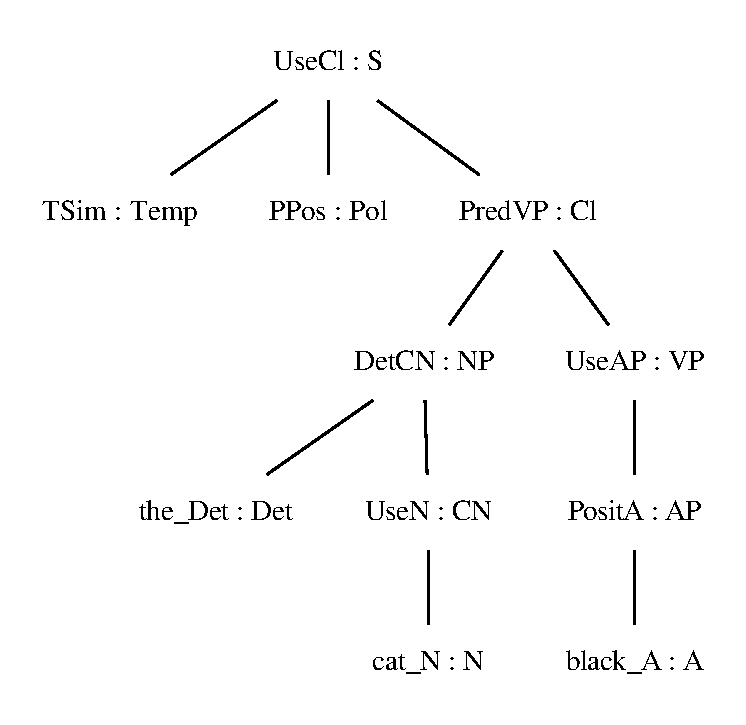
\includegraphics[width=0.5\linewidth]{figure/cat_is_black_gf.eps}
  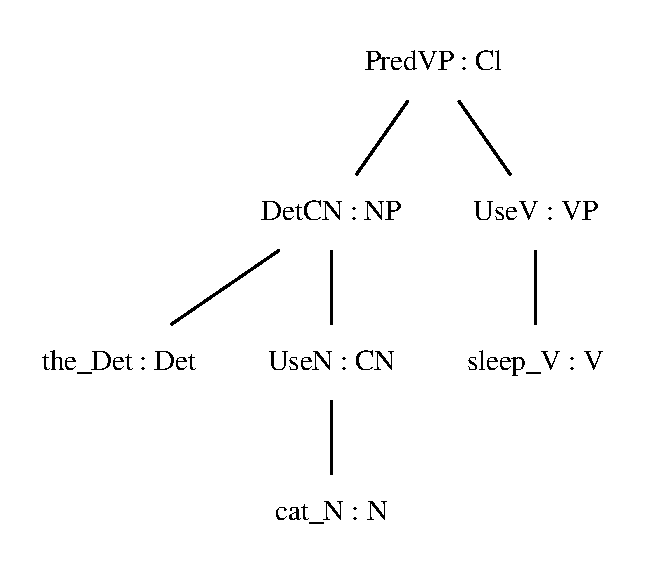
\includegraphics[width=0.5\linewidth]{figure/cat_sleeps_cl.eps}
  \caption{The sentence ``The cat sleeps'' analyzed as a GF tree}
  \label{fig:cat_sleeps_gf}
\end{figure}


% NOTES:
% "The cat is black" vs "The cat is not black" corresponds to PPos vs PNeg
% ud2gf would have trouble differentiating between these because it's only in parameters
% Macros UseCl_NegCop and UseCl_Sim corresponds to the different versions
% These allows the information to be preserved, despite there not being any explicit GF function for the word ``not''
%
% Negative:
% UseCl_NegCop (StrNeg "not") (PredVP (DetCN_theSg (StrThe "the") (UseN cat_N)) (UseAP_Cop (StrCop "be") (PositA black_A)))
% Positive:
% UseCl_Sim (PredVP (DetCN_theSg (StrThe "the") (UseN cat_N)) (UseAP_Cop (StrCop "be") (PositA black_A)))

% #auxfun UseCl_Sim cl : Cl -> S = UseCl TSim PPos cl ; head
% #auxfun UseCl_Ant have cl : Have -> Cl -> S = UseCl TAnt PPos cl ; aux head
% #auxfun UseCl_NegSim do neg cl : Do -> Neg -> Cl -> S = UseCl TSim PNeg cl ; aux advmod head
% #auxfun UseCl_NegAnt have neg cl : Have -> Neg -> Cl -> S = UseCl TAnt PNeg cl ; aux advmod head
% #auxfun UseCl_NegCop neg cl : Neg -> Cl -> S = UseCl TSim PNeg cl ; advmod head

% #auxfun UseAP_Cop cop comp : Cop -> AP -> VP = UseAP comp ; cop head

% #auxcat Cop AUX
% #auxcat Do AUX
% #auxcat Have AUX
% #auxcat Neg PART

% Syncategorematic words:
% #word not not Polarity=Neg
% #word does  do  Mood=Ind|Number=Sing|Person=3|Tense=Pres|VerbForm=Fin
% #word is   be  Mood=Ind|Number=Sing|Person=3|Tense=Pres|VerbForm=Fin
% #word would would  VerbForm=Fin
% #word will  will VerbForm=Fin

% Syncategorematic lemmas:
% #lemma UseCl,UseQCl,ImpVP not Neg advmod head
% #lemma UseAP,UseAdv,UseNP be Cop cop head
% #lemma PredVP have Have aux head
% #lemma PredVP,ImpVP do Do aux head

%  - strengths and weaknesses
%
\section{Differences between GF and UD}
% Strengths and weaknesses


% % Grammatical Framework has [some] advantages for [use-case], so it would be useful to be able to parse using UD and then get out a GF tree. A
GF is very strict when it comes to following grammar and spelling, which means that it will often refuse to parse sentences if they contain even the smallest error. UD on the other hand uses machine-learning to give some parse tree for all sentences regardless of how many errors they have.

While the machine-learning-based approach of UD allows it to guess the correct tree better for ambiguous sentences and allows it to handle grammatically incorrect sentences better, GF is much more capable when
it comes to performing transformations on the sentences, while maintaining correct morphology and grammar. This makes it attractive to parse sentences
using UD and then convert the parsed trees to GF trees in order to perform further transformations.


% Anteckningar

% UD har en massa manuellt annoterade träd som folk har tränat maskininlärningssystem på

% GF är mer strikt och kräver att grammatiken följs exakt och stavfel och små grammatikfel kommer inte

% UD är mer robust för fel och kommer alltid ge resultat oavsett om saker inte följs exakt och ger sin bästa gissning

% GF är mer exakt och förutsägbar, så buggar går bättre att anylysera och fixa

% Med GF kan man transformera meningar och träd på mycket fler sätt, till exempel kan ett påstående göras till en fråga bara genom att wrappa hela meningen med en MkQuestion funktion och då kommer automatiskt GF fixa alla morfosyntaktiska ändringar, så som att ändra ordföljd eller

% använder automatiskt rätt genus om man byter ut ett ord till ett annat

% abstrakt träd är oberoende av språk

% RGL beskriver morfosyntax för språk medan en applikationsgrammatik kan vara på högre nivå och ge mer ideomatiska översättningar och det beskrivs i termer av den abstrakta syntaxen för resursgrammatiken



% % Maybe mention the macros in the labels files

% % There exists a naive implementation based on a brute-force algorithm \cite{kolachina-ranta-2017}

% % Briefly describe and motivate the project, and convince the reader of the importance of the proposed thesis work.
% % A good introduction will answer these questions: Why is addressing these challenges significant for gaining new knowledge
% % in the studied domain? How and where can this new knowledge be applied?


\subsection{Useful synthesis between UD and GF}

% \todo[inline]{explain about gf-ud, the old-old version, the new-old version and my developments on that}

Prior to this work there existed a proof-of-concept implementation of a tool for converting between the trees for GF and UD,
with the help of so-called labels-files containing annotations which describe the mapping between UD labels and GF functions,
called gf-ud, which contains both a component for converting from UD to GF, called ud2gf\cite{kolachina-ranta-2017}\footnotemark[1]
and a component for converting from GF to UD, called gf2ud\cite{kolachina-ranta-2016}\footnotemark[1]. This work will focus on the ud2gf component.

\footnotetext[1]{These references apply to an older version of gf-ud, from before the one this thesis is based on. A part of the goal of this thesis is to document the later version in addition to documenting the changes made in the process of this thesis.}

% \todo{these references apply to an older version of gf-ud, from before the one I was working on. a part of the goal of this thesis is to document the old-new version that my changes was based on}

% The labels files can also contain macros, which allows constructing virtual GF functions during the translation from UD, which will be expanded to real GF functions at the end of the translation.
% These can, among other uses, be used to preserve information from the UD labels about subtrees, which can then be used at later points of the transformation to ensure that the desired GF tree is produced.

\subsection{Applications for the synthesis of UD and GF}

The gf-ud tool has been used for both translation and semantics\cite{ranta-al-2020}. %\todo{actually explain this}
Another application has been in concept alignment\cite{masciolini-ranta-2021}.
It has also been used to analyze legal texts as a part of a Controlled Natural Language for law\cite{listenmaa-etal-2021-towards}.

\section{What problem does ud2gf solve?}
% \todo[inline]{This is the main focus of the intro}
%
% \todo[inline]{Add edge labels to graph}
%
% \todo[inline]{write this text}

One problem within \ac{NLP} is converting from text to logic. There are several different paths one could take, each with their own issues, see \autoref{fig:text-to-logic} for an overview. The tool gf2ud makes it possible to get the robust parsing available for dependency trees and the ease of conversion to logic of Abstract Syntax Trees.

\begin{figure}[H]
    \centering
    % \includegraphics{}
    % \missingfigure{Graph of possible ways to convert from text to logic}
    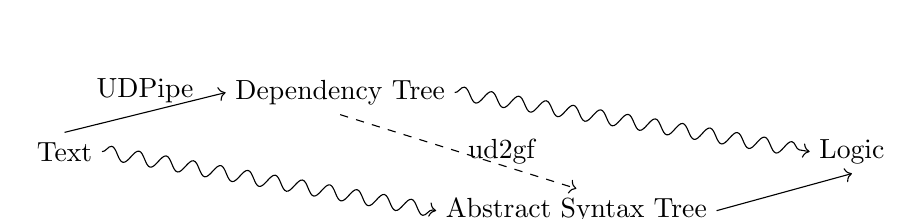
\begin{tikzpicture}
        \tikzset{snake it/.style={decorate, decoration=snake}}
		\node(Text) at (-5, 0) {Text};
		\node(DT) at (-1.5, 0.75) {Dependency Tree};
		\node(AST) at (1.5, -0.75) {Abstract Syntax Tree};
		\node(Logic) at (5, 0) {Logic};
		\draw[->] (Text.north) to node[above] {UDPipe} (DT.west);
		\draw[->, snake it] (Text.east) to (AST.west);
		\draw[->] (AST.east) to (Logic.south);
		\draw[->, snake it] (DT.east) to (Logic.west);
		\draw[->,dashed] (DT.south) to node[right] {ud2gf} (AST.north) ;
    \end{tikzpicture}
    \caption{An overview of how gf2ud can be helpful in converting from text to logic}
    \label{fig:text-to-logic}
\end{figure}

Converting from text to dependency trees is a solved problem\cite{Nivre2006,straka-etal-2016-udpipe,kanerva-etal-2020-turku}. Converting from AST to logic is a solved problem\cite{Montague1973-MONTPT-4,ranta-2004b,ranta2022end}. Converting from dependency trees to logic is a difficult problem\cite{reddy2016transforming,ranta2017explainable}. Converting from natural language text directly to AST is a difficult problem\cite{ranta-2011c,bernardy-stergios-2017,landin-1966-next-700,curry1961some,Montague1973-MONTPT-4}. By converting from DT to AST ud2gf allows us to use the two solved problems to get a path from text to logic.


% Från mallen


% This chapter presents the section levels that can be used in the template.
%
% \section{Section levels}
% \autoref{tab:sections} presents an overview of the section levels that are used in this document. The number of levels that are numbered and included in the table of contents is set in the settings file \texttt{Settings.tex}. The levels are shown in Section \ref{Section_ref}.
%
% This is a new paragraph and should have proper parskip or indentation. Don't forget to cite your sources~\cite{listenmaa-etal-2021-towards}. % '~' becomes space which cannot line break.
%
% \begin{table}[h]
% \centering
% \caption{Section levels} % Table text above table.
% \begin{tabular}{ll} \hline
% Name & Command\\ \hline
% Chapter & \textbackslash\texttt{chapter\{\emph{Chapter name}\}}\\
% Section & \textbackslash\texttt{section\{\emph{Section name}\}}\\
% Subsection & \textbackslash\texttt{subsection\{\emph{Subsection name}\}}\\
% Subsubsection & \textbackslash\texttt{subsubsection\{\emph{Subsubsection name}\}}\\
% %Paragraph & \textbackslash\texttt{paragraph\{\emph{Paragraph name}\}}\\
% %Subparagraph & \textbackslash\texttt{paragraph\{\emph{Subparagraph name}\}}\\ \hline\hline
% \end{tabular}
% \label{tab:sections}
% \end{table}

% \section{Section} \label{Section_ref}
% \subsection{Subsection}
% \subsubsection{Subsubsection}
% \paragraph{Paragraph}
% \subparagraph{Subparagraph}


% THEORY
% % CREATED BY DAVID FRISK, 2016
\chapter{Theory}

In the following sections, examples of a figure, an equation, a table and a source code listing  are shown.

\section{Figure}
\begin{figure}[H]
\centering
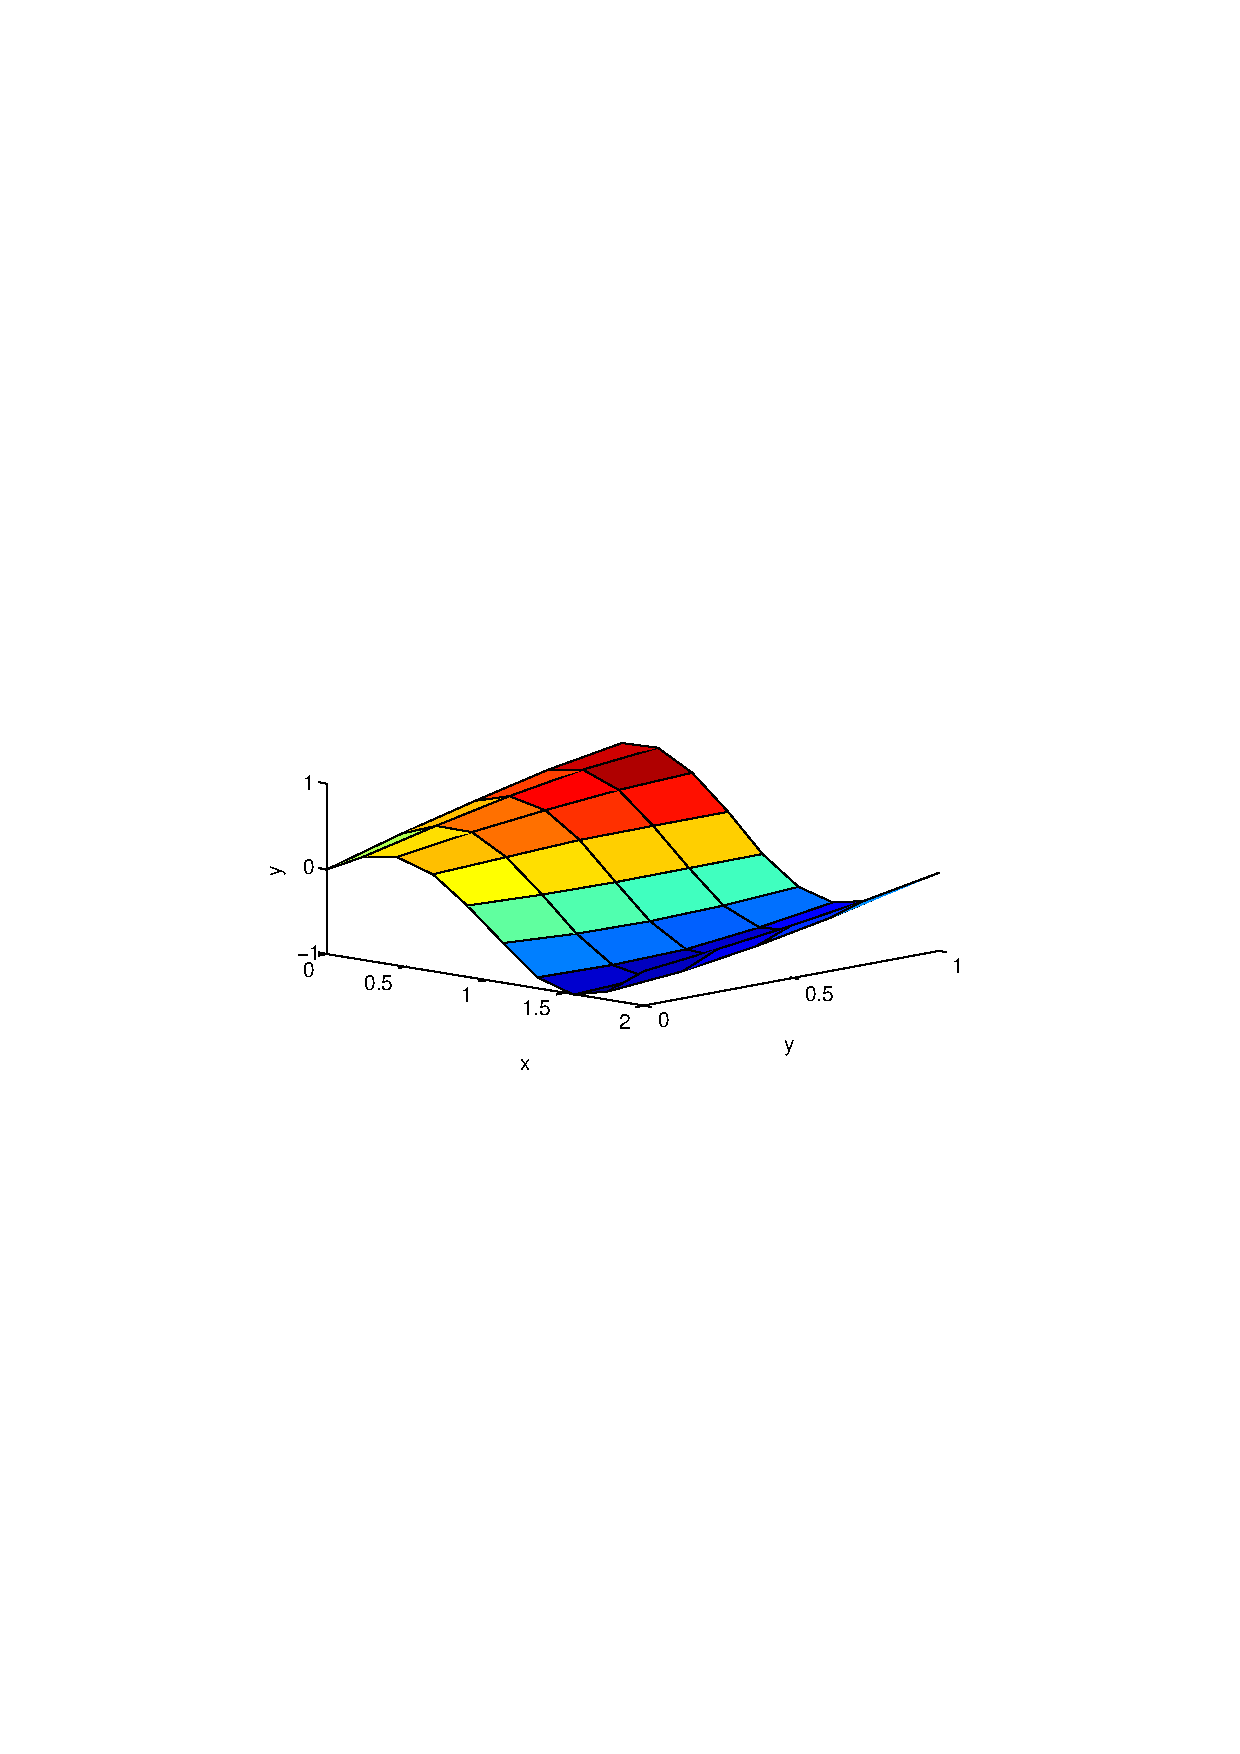
\includegraphics[width=0.45\linewidth, trim=3cm 11cm 3cm 11cm]{figure/X.pdf}
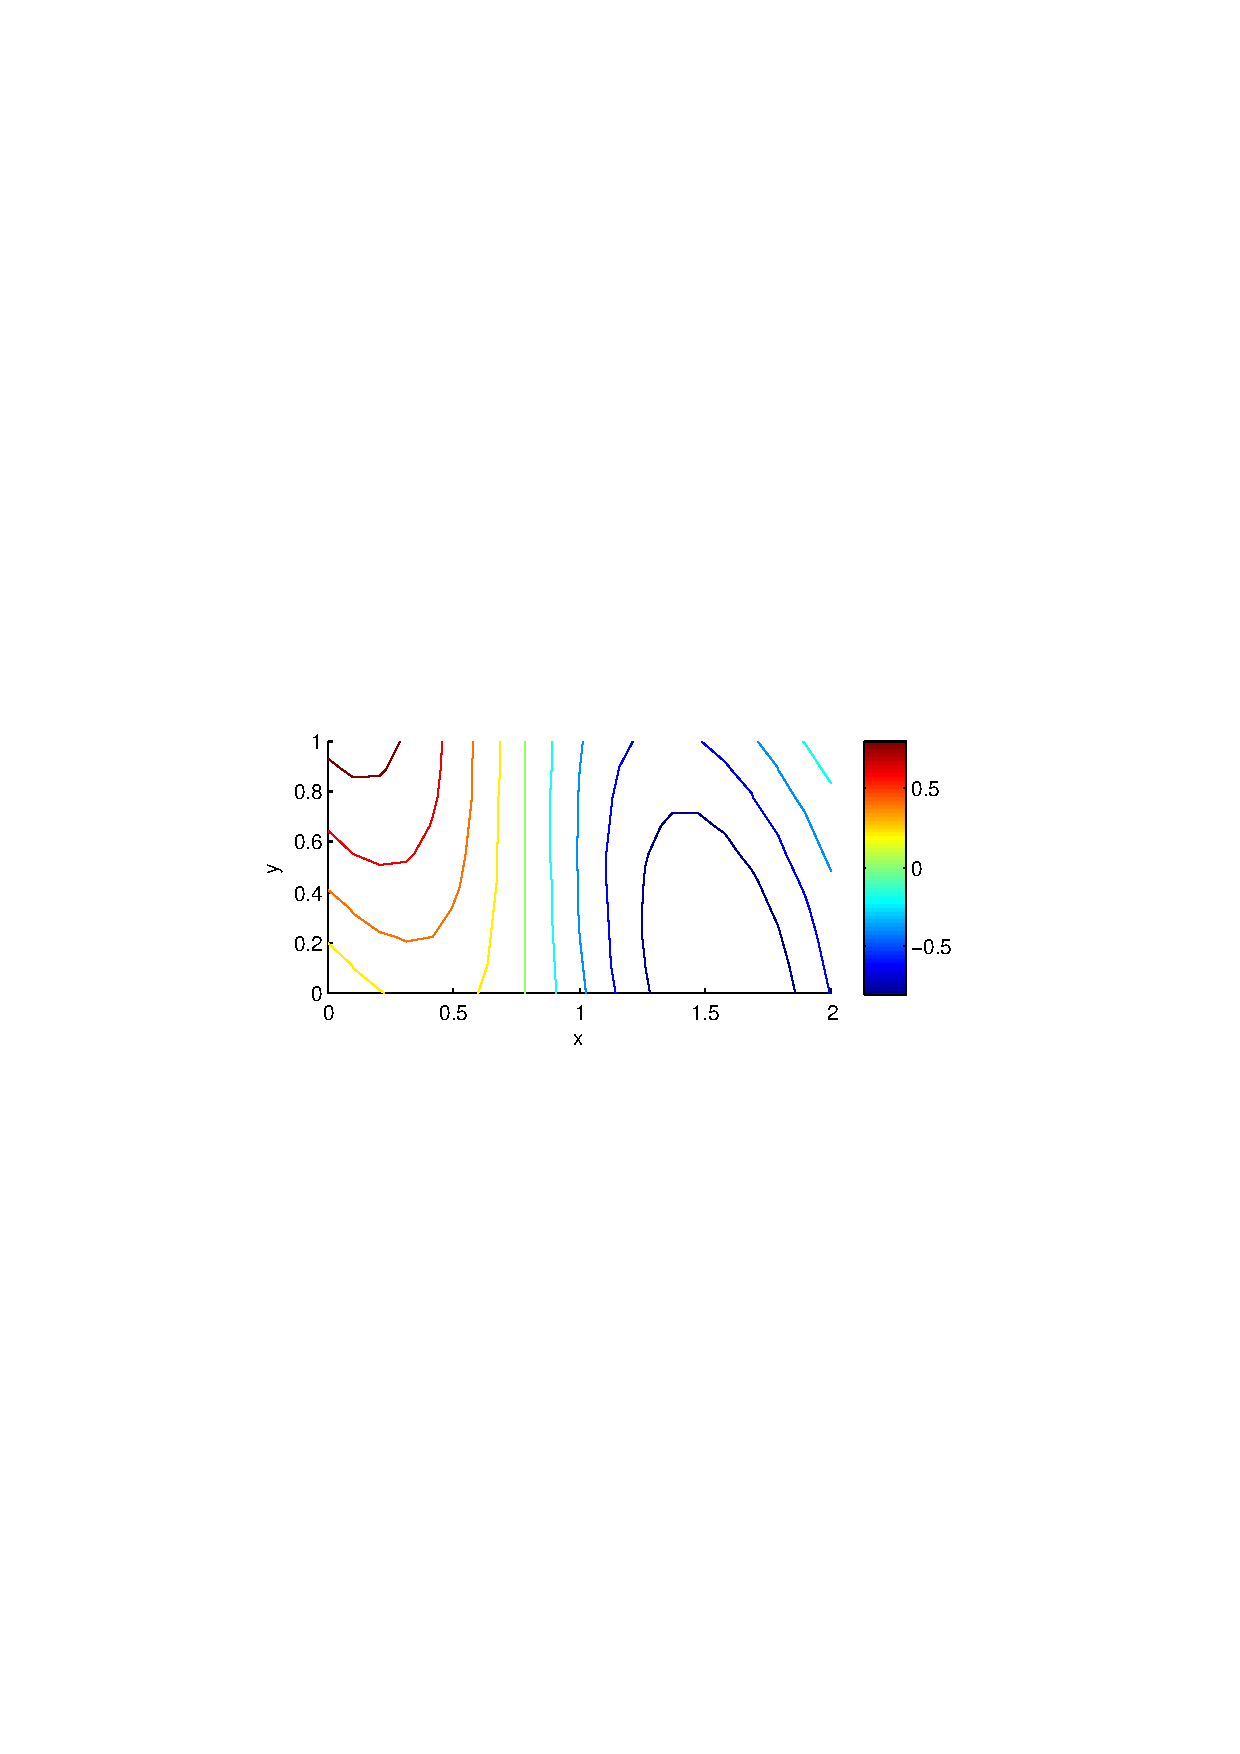
\includegraphics[width=0.45\linewidth, trim=3cm 11cm 3cm 11cm]{figure/Y.pdf}
\caption{Surface and contour plots showing the two dimensional function $z(x,y)=\sin(x+y)\cos(2x)$.} % Figure text below figure
\end{figure}

\section{Equation}
\begin{equation}
f(t)=\left\{ \begin{array}{ll}
1,~~~~ & t< 1 \\
t^2 & t\geq 1
\end{array}\right.
\end{equation}

\section{Table}
\begin{table}[H]
\centering
\caption{Values of $f(t)$ for $t=0,1,\dots 5$.}
\begin{tabular}{l|llllll} \hline\hline
$t$ & 0 & 1 & 2 & 3 & 4 & 5 \\ \hline
$f(t)$ & 1 & 1 & 4 & 9 & 16 & 25 \\ \hline\hline
\end{tabular}
\end{table}

\section{Chemical structure}
\begin{center}
\chemfig{X*5(-E-T-A-L-)}
\end{center}


\section{Source code listing}
\begin{minted}[frame=single]{matlab}
% Generate x- and y-nodes
x=linspace(0,1); y=linspace(0,1);

% Calculate z=f(x,y)
for i=1:length(x)
 for j=1:length(y)
  z(i,j)=x(i)+2*y(j);
 end
end
\end{minted}

\subsection{Other alternatives to the Theory chapter}
Sometimes, it is more appropriate to name this chapter Background.

At CSE, there exists a large span of different types of thesis works. Sometimes it is more appropriate to join the Theory and Methods chapters, sometimes the Theory chapter would be so small that it should be a subsection. Talk to your supervisor to find the most appropriate structure for your thesis.


\chapter{Background and Problem}

% - old ud-gf
% - newer naive approach - github + article 2017
%   - limitations
%   - performance


% Background to the assignment. Why is it relevant?
\section{Background}
\section{Problem}
% The formulation of the problem at hand and, the assignment. This should include an extended version of the scientific problem definition and references to knowledge within the area given in the thesis proposal.

% What has been done before and what remains to be done

% 2. Background & Problem
% - old ud-gf
% - newer naive approach - github + article 2017
%   - limitations
%   - performance

The current ud2gf implementation has some limitations. There are three main problems this work tries to fix.

The first problem is that it quickly becomes extremely slow for sentences with more than a couple of words and/or
when using large GF-grammars, e.g. GF-grammars containing Wordnet\cite{angelov2016predicting}. \\
The second problem is that if the structure differs too much between the representation of a sentence in UD format and as a GF tree, it is not possible to describe the required transformation in the current "labels file" language. See section \ref{sect:flex} below for more details. \\
The third problem is that it can sometimes be difficult to figure out why a rule in a labels-file is not firing, so it would be useful to have a debugging tool to help diagnosing such issues.


\subsection{Flexibility}\label{sect:flex}

As an example of a phrase that can be difficult to convert using the old gf2ud, let us consider the adjectival phrase "cute, fluffy and furry"
would be described in UD format as in Figures \ref{fig:ud_cute_text} and \ref{fig:ud_cute}.


\begin{figure}
    \begin{verbatim}
    1  cute  cute  ADJ  JJ  Degree=Pos  0  root  _  FUN=cute_A
    2  ,  ,  PUNCT  ,  _  3  punct  _  _
    3  fluffy  fluffy  ADJ  JJ  Degree=Pos  1  conj  _  FUN=fluffy_A
    4  and  and  CCONJ  CC  _  5  cc  _  FUN=and_Conj
    5  furry  furry  ADJ  JJ  Degree=Pos  1  conj  _  FUN=furry_A
    \end{verbatim}
    % \begin{tabular}{|c|c|c|c|c|c|c|c|c|c|}
    % \hline
    % 1 & cute & cute & ADJ & JJ & Degree\=Pos & 0 & root & \_ & FUN\=cute\_A \
    % \hline
    % 2 & , & , & PUNCT & , & \_ & 3 & punct & \_ & \_ \
    % \hline
    % 3 & fluffy & fluffy & ADJ & JJ & Degree\=Pos & 1 & conj & _ & FUN\=fluffy\_A \
    % \hline
    % 4 & and & and & CCONJ & CC & \_ & 5 & cc & \_ & FUN\=and\_Conj \
    % \hline
    % 5 & furry & furry & ADJ & JJ & Degree\=Pos & 1 & conj & \_ & FUN\=furry\_A \
    % \hline
    % \end{tabular}
    \caption{The phrase "cute, fluffy and furry" as a textual UD tree}
    \label{fig:ud_cute_text}
\end{figure}

\begin{figure}
    \centering
    % \begin{dependency}
  \begin{deptext}[column sep=0.4cm]
      cute \& , \& fluffy \& and \& furry \\
    {\tt ADJ}\&{\tt PUNCT}\&{\tt ADJ}\&{\tt CCONJ}\&{\tt ADJ} \\
  \end{deptext}
  \depedge{2}{1}{punct}
  \depedge{0}{2}{conj}
  \depedge{4}{3}{cc}
  \depedge{0}{4}{conj}
\end{dependency} \\
    % \includesvg{ud-annotatrix-corpus.svg}
    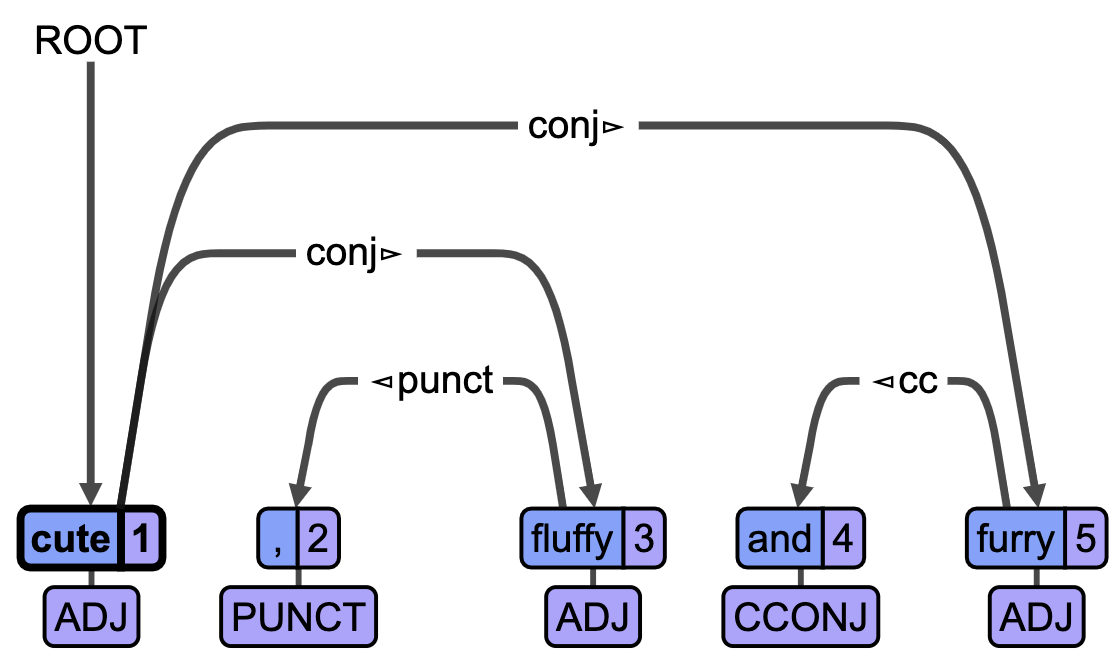
\includegraphics[width=0.7\textwidth]{figure/ud_cute.png}
    \caption{The phrase "cute, fluffy and furry" as a UD tree in graphical format}
    \label{fig:ud_cute}
\end{figure}
% \include{}

\begin{figure}
    \centering
    % \begin{dependency}
  \begin{deptext}[column sep=0.4cm]
      cute \& , \& fluffy \& and \& furry \\
    {\tt ADJ}\&{\tt PUNCT}\&{\tt ADJ}\&{\tt CCONJ}\&{\tt ADJ} \\
  \end{deptext}
  \depedge{2}{1}{punct}
  \depedge{0}{2}{conj}
  \depedge{4}{3}{cc}
  \depedge{0}{4}{conj}
\end{dependency} \\
    % \includesvg{ud-annotatrix-corpus.svg}
    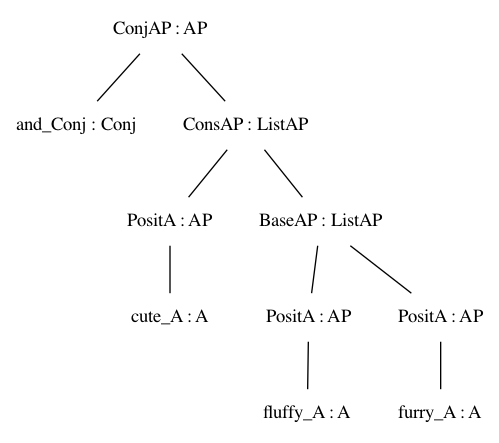
\includegraphics[width=0.7\textwidth]{figure/cute_gf.png}
    \caption{The phrase "cute, fluffy and furry" as a GF tree in graphical format. }
    \label{fig:gf_cute}
\end{figure}

The GF version of the same tree, shown in Figure \ref{fig:gf_cute}, would look like this:

\begin{verbatim}
ConjAP and_Conj (ConsAP (PositA cute_A)
                        (BaseAP (PositA fluffy_A) (PositA furry_A)))
\end{verbatim}
Here we can see that in UD, the word "cute" is in the root, while the conjunction "and" is at the bottom of the tree, while in GF the conjunction is a direct child of the root. This transformation can not be preformed by the simple single-layer transformations that are available in the current macro-system for labels files.

% Ideas:
%
% - Limits on how to transform trees - solution: extend language. currently hack using lambda calculus, but maybe better macros
%
% - Evaluate effectiveness of tool
%
% - (somewhere mention the performance boosts and analyse the complexity of it)

% This section is optional. It may be used if there is a need to describe the problem that you want to solve in more technical
% detail and if this problem description is too extensive to fit in the introduction.

% From elsewhere:
% - Background: GF \cite{ranta-2004}, UD \cite{nivre-etal-2016-universal},
%   - previous work: gf2ud \cite{kolachina-ranta-2016}, ud2gf \cite{kolachina-ranta-2017}
% - Describe the new algorithm
% - Extending the macro language
%   - Need for improvement: to match "fluffy and cute" needs 2 levels of nesting
%   - Solution: continuations
% - Case study: legal language

The translation described by a labels file is not one-to-one and there are often many possible GF trees that a UD tree could be translated to. The possible trees are currently ranked by completeness, as in how many of the words are included in the generated tree. However this ranking is incomplete and in case two possible trees, with the same GF category, cover the same words, an arbitrary tree will be chosen. A better choice could be to also check the linearization of these trees and rank those whose linearization is more similar to the original string higher. It would also be possible to completely exclude trees with differing linearization, but that would run counter to the goal of robustness.


% 3. The new algorithm
% - definitions
% - examples
% - how annotations work

% \section{Context}
% \todo[inline]{What's the difference between this and intro?}
% This work is mostly a continuation of the work in \cite{kolachina-ranta-2017}.

% A practical problem for which this tool can be useful can be found in \cite{listenmaa-etal-2021-towards}. In the Future Work section, under "Robust fall-back options", gf2ud is mentioned as a possible solution to making the parser more robust.

% % Use one or two relevant and high quality references for providing evidence from the literature that the proposed study indeed
% % includes scientific and engineering challenges, or is related to existing ones. Convince the reader that the problem addressed
% % in this thesis has not been solved prior to this project.

% Aim for the work. What should be accomplished?
\section{Goals and Challenges}

% try to preserve as much information as possible from the UD tree

% do this in an efficient way

% \todo[inline]{No longer relevant for final report?}

% \todo[inline]{Change this so it's clear that it has already been done}

1. Analyze algorithms and improve performance. The main challenge here is to find an algorithm for finding matching trees without exponential complexity on the number of children of a node in the UD tree.

2. Improve flexibility of macro language, allowing changing the structure of the trees while translating from GF to UD. One challenge here is in figuring out either how to change the algorithms to support these more advanced transformations or to find a way to allow them without needing to change the algorithms.

3. Write a debugging tool, which analyzes exactly what it is that prevents a rule in a labels-file from firing or what prevents that tree from being selected.
One challenge here is how to explain to the user the issue for all the possible things that can go wrong.
There is also an engineering challenge in making an algorithm that figures out what went wrong and why.
% either repeating the steps of the algorithm in order to find the issues or transforming the algorithm in a way that they can explain what went wrong

4. Document the version of the tool on which this work is based on, which had changed since what was written in \cite{kolachina-ranta-2017}


\subsection{Future work}

5. If there is time, update the algorithm to look at the linearization in order to try to select trees that match the original string as closely as possible and evaluate what difference this makes. This is only possible with improved performance from goal 1, but keeping it fast will still be a challenge. There are also some challenges here in how it should interact with the advanced macros in goal 2. We also need to handle when a GF tree has multiple linearizations, e.g. if it results in a conjugation table.

% % improve

% % Analyse the complexity of old and new algorithm, evaluate effectiveness of ...

% % Describe your contribution with respect to concepts, theory and technical goals. Ensure that the scientific and engineering
% % challenges stand out so that the reader can easily recognize that you are planning to solve an advanced problem.


% Limitations. What should be left out and why?
\section{Limitations}

Only the direction of converting UD trees to GF trees is studied here, because that is what was relevant to the application at hand. Furthermore, the two directions are almost completely independent in the implementation.

% I normalfallet behöver avgränsningarna inte motiveras.

% Limit the work mostly to what has already been done

% Har gjort:
%

%  \todo{why?}

% \todo[inline]{other limitations?}


% METHODS
% CREATED BY DAVID FRISK, 2016
\chapter{Methods}
Methods text.



\section{Approach}
% Method of accomplishment. How should the work be carried out?

These methods were used for the different parts of the project

% \todo[inline]{Change these to past tense}
\subsection{Performance}

1. Finding the main source of slowness, which was done with profiling.

2. Analysing the current algorithms, which are based on brute force, trying all combinations, with some simple filtering.

3. Finding a better algorithm, which avoids exploring paths that could never be the correct answer and which avoids duplicate work.

4. Analysing the algorithmic complexity of both the new and the old algorithm and testing the practical performance to confirm the results.

\subsection{Flexibility}

In order to allow changing the shape of trees when translating from UD to GF, the macro language needs to be expanded.
A first prototype of this with minimal code changes has been done by making macro expansion recursive and then representing the code for the transformation in Church-encoding, inspired by lambda-calculus.

This approach can be evaluated by seeing how well it covers different tree shape changes for different trees one would encounter.

It could also be worthwhile to make a more user-friendly version of the advanced macros that can be understood without knowing about Church-encoding

\subsection{Debugging tool}
Going through each component of the algorithms in order to find where applying a rule can go wrong and add detection for them. Additionally trying out the debugging tool on a real grammar, e.g. in the context of \cite{listenmaa-etal-2021-towards}, in order to find edge-cases which were not handled by the debugging tool.

% Trial and error, whenever a problem arises that the tool doesn't find a helpful explanation for, try to add support for it.

\subsection{Linearization-aware translation}
Here we need a way to determine which linearization is actually closer and when to keep multiple options for a later stage of the translation. Some care also needs to be taken in determining which trees can be discarded and which ones need to remain available for a later stage.

Evaluating if the results are better with this version can be done in a large part by comparing the input string with the resulting string after translating to GF and linearizing.


% The old algorithm
\chapter{The old algorithm}

% \todo[inline]{Move to before methods?}
% \todo[inline]{Or is the goal of the paper to describe this? probably not}

% Explain what the old algorithm does
% Explain what has changed


% The new algorithm is based on

% \section{Definitions}



% TODO from meeting with Aarne
% DONE Rename chapter to old algorithm make new chapter for new algorithm
% The kind of algorithm Forward something,  parsing
% One UD tree can be many GF trees

% Example of UD corresponding to several GF trees:
% grande famille francaice

% coffee or tea and soup
% not ambigous in UD, but the phrase is ambigous

% Can linearize wrong

% Church encoding of pairs

% Link to github

% Exempel före definition

% Synkategorimatiska ord behöver särskild syntax för att dom inte har någon egen kategori
% kategorimatiska ord är lexikal funktion (utan argument)
% synkategorimatiska ord kommer från linjariseringsregler för funktioner tar argument

% diskontinueliga saker, e.g. V2 med prepositioner är syncat
% multiword expressions är en nod i GF men olika i UD

% konjunktioner: första ordet är förälder medan alla andra ord har komma eller konjunktion som barn

% Intressant idé: Definiera en mappning mellan två GF-grammatiker

% Redundans: koppling åt båda håll för syncats

% Old version of gf2ud still exists in gf-shell

% Half time report

% Describe the annotation
% #fun
% #cat
% #auxfun - macros
% #auxcat

% Syncat: #morpho, #lemma, #word
% Used both directions

% Parameters aren't automatically handled, but you need to create auxfuns


% Auxfun are not type checked

% Needed for halftime report:
% Write what the empty chapters will contain

\todo[inline]{Where is the old algorithm from?}

% \todo[inline]{Signposting: In this section we will explain ...}

In this chapter, we first explain the annotations that are used to describe the mapping between \ac{GF} trees and \ac{UD} trees, then we present a high level overview of the algorithm followed by going through a concrete example of how the algorithm works. Finally, we discuss some limitations of the old algorithms, which we cover solutions of in the next chapter.

\section{Overview}

% \todo[inline]{fix this}
% The whole process goes like this: first we do X (section XXX, then we do Y (section YYY)

\ac{GF} trees consist of functions and categories, \ac{UD} trees consist of \ac{POS} annotations and dependency labels and some optional extra annotation.

The ud2gf tool uses annotations in a so called \verb|.labels|-file to describe the relation between the \ac{UD} labels and the \ac{GF} functions. These annotations give constraints, which are used to decide which \ac{GF} functions can be applied where. The algorithm starts by parsing each individual word using \ac{GF} for each of the possible categories according to the annotations and the Part of Speech. After that the algorithm tries to recursively apply as many functions as possible, following the constraints from the annotations and the \ac{UD} tree structure. When multiple trees of the same category are generated at the same location in the \ac{UD} tree, the most complete ones are selected. Here, completeness is a partial order measured in terms of how many words are included in the selected tree. A tree that contains all words that another tree has is considered more complete. Finally backup functions are inserted to include the words that were not included in (one of) the most complete trees.

\section{How annotations work}\label{sec:annotations-intro}

In order for the program to know which \ac{UD} \ac{POS} corresponds to which \ac{GF} categories (can be multiple) and how the \ac{GF} functions relate to the \ac{UD} dependency labels, we need to supply annotations which describe these correspondences. Most of these annotations are bidirectional and are used both by ud2gf and gf2ud. A complete description of these annotations can be found in \autoref{app:annotation}.

First we have the \lstinline{#cat} annotation, which describes the mapping from \ac{GF} categories and \ac{UD} Part of Speech labels:

\begin{lstlisting}
    #cat GFCategory UD_POS
    #cat N NOUN
\end{lstlisting}

Secondly we have the \lstinline{#fun} annotation, which describes \ac{GF} functions and which \ac{UD} dependency label each argument of the function should have (see \autoref{fig:DetCN} for graphical representation of such an annotation). The type signature of the \ac{GF} function is also required. Each function needs to have exactly one argument with the label \lstinline{head}, corresponding to the head of the current subtree of the \ac{UD} tree, and any number of arguments corresponding to the direct children of that head in the \ac{UD} tree, which are labeled with their corresponding \ac{UD} dependency labels. It is also possible to add other \ac{UD} annotations in brackets to a label.

% \todo[inline]{How to give this listing a number and a label}
\begin{lstlisting}
    #fun GFFunctionName : FirstArgumentCat -> SecondArgumentCat -> ReturnCat ; first_ud_label second_ud_label
    #fun UseN : N -> CN ; head
    #fun DetCN  : Det -> CN -> NP ; det  head
\end{lstlisting}

The function \lstinline{UseN} only has a single argument (of type \lstinline{N}), so that is required to be the head, while the function \verb|DetCN| has two arguments, of types \verb|Det| and \verb|CN|, the first of which has the dependency label \verb|det|, while the second is the head. An illustration of this can be seen in \autoref{fig:DetCN}.

\begin{figure}
    \centering
    \begin{dependency}
        \begin{deptext}[column sep=0.4cm]
              % the \& cat \\
            % {\tt Det}\&{\tt CN}\&{\tt NP}\\
            {\tt Det}\&{\tt CN}\\
        \end{deptext}
        \depedge{2}{1}{det}
        \deproot{2}{head}
        % \wordgroup{1}{1}{2}{args}
        % \wordgroup{1}{3}{3}{res}
        % \groupedge[edge below]{args}{res}{\texttt{DetCN}}{2ex}
        \node (arg1) [below of = \wordref{1}{1}, yshift = -1ex]  {\texttt{Det}};
        \node (arg2) [below of = \wordref{1}{2}, yshift = -1ex]  {\texttt{CN}};
        \node (result) [right of = arg2, xshift = 1ex]  {\texttt{NP}};
        \node (function) [left of = arg1, xshift = -1.5ex]  {\texttt{DetCN :}};
          % Det} -> \subnode{arg2}{CN} -> NP}};
        \draw [->, thick] (arg1) -- (arg2);
        \draw [->, thick] (arg2) -- (result);
        \draw [->, very thick, dashed, gray] (arg1) -- (\wordref{1}{1});
        \draw [->, very thick, dashed, gray] (arg2) -- (\wordref{1}{2});
    \end{dependency} \\
    \caption{The UD shape that the function \texttt{DetCN} matches against.}
    \label{fig:DetCN}
\end{figure}

Both of these annotations are bidirectional and language-independent, since they only refer to the abstract syntax in \ac{GF}.

%% TODO: Other

% The different kinds of annotations in labels files
% Funs


%\section{Examples}

% When converting the sentence ``The cat is black'', from UD format to a GF format using ud2gf something happens
%
% \begin{lstlisting}
% # gf, (gf2ud) original GF tree:
% UseCl TSim PPos (PredVP (DetCN the_Det (UseN cat_N)) (UseAP (PositA black_A)))
% # an3, (gf2ud) final annotated tree with nonlocal operations:
% @4: black black ADJ _  black_A A root
%     @2: cat cat NOUN Number=Sing  cat_N N nsubj
%         @1: the the DET _  the_Det Det det
%     @3: is be AUX Mood=Ind|Number=Sing|Person=3|Tense=Pres|VerbForm=Fin  UseAP VP cop
%
% # ut, tree-structured UD tree:
% 4       black   black   ADJ     A       _       0       root    _       FUN=black_A
%     2   cat     cat     NOUN    N       Number=Sing     4       nsubj   _       FUN=cat_N
%         1       the     the     DET     Det     _       2       det     _       FUN=the_Det
%     3   is      be      AUX     VP      Mood=Ind|Number=Sing|Person=3|Tense=Pres|VerbForm=Fin   4       cop     _       FUN=UseAP
%
% # ud, UD tree in CoNLLU format:
% # sent_id = gfud1000001
% # text = the cat is black
% 1       the     the     DET     Det     _       2       det     _       FUN=the_Det
% 2       cat     cat     NOUN    N       Number=Sing     4       nsubj   _       FUN=cat_N
% 3       is      be      AUX     VP      Mood=Ind|Number=Sing|Person=3|Tense=Pres|VerbForm=Fin   4       cop     _       FUN=UseAP
% 4       black   black   ADJ     A       _       0       root    _       FUN=black_A
%
% \end{lstlisting}

\section{Overview of algorithm}\label{sec:overview-of-algorithm}

We start with a \ac{UD} tree (e.g. \autoref{fig:the_black_cat_ud}), then we first map each \ac{POS} label into a \ac{GF} category and then assign lexical entries to each node in the tree according to those categories. For example, the string ``cat'', with \ac{POS} ``NOUN'' would become \lstinline|cat_N : N|, which is a nullary (takes no arguments) \ac{GF} function of type/category \lstinline|N|. This is done through \ac{GF}'s built-in parse function. In some cases, there are multiple possible \ac{GF} expressions of the correct type and linearization, in these cases all of the possibilities are added.

Now we have a \ac{UD} tree with a list of \ac{GF} trees at each node (\autoref{fig:the_black_cat_ud_gf}). We process the tree bottom up, starting with the leaf words and then the words for which all the children/dependents have been processed.
% We start traversing the tree, depth first, when we reach a leaf, we start processing the leaf. Afterwards we

The main loop at each word consists of trying to apply each of the available \ac{GF} functions to each of the available trees for that word, combined with as many trees from unused dependent words as the function requires. For each combination, the algorithm checks that the used trees match the annotations for the function in both in \ac{GF} category and \ac{UD} dependency labels. Each of the generated trees are added to the list of trees for the current word.
%  go through all the available functions and apply as many as possible and add the result to our list
When no more functions can be applied, we go to the next word in the tree.

\subsection{Example: The black cat}

For a very simple initial example, we start with the noun-phrase ``the black cat'', which has the following \ac{UD} representation:

\begin{figure}[H]
    \centering
    %% the black cat
    \setlength{\unitlength}{0.2mm}
    % \begin{picture}(158.0,90.0)
    %   \put(0.0,0.0){the}
    %   \put(37.0,0.0){black}
    %   \put(92.0,0.0){cat}
    %   \put(0.0,15.0){{\tiny DET}}
    %   \put(37.0,15.0){{\tiny ADJ}}
    %   \put(92.0,15.0){{\tiny NOUN}}
    %   \put(56.0,30.0){\oval(88.73913043478261,66.66666666666667)[t]}
    %   \put(11.630434782608695,35.0){\vector(0,-1){5.0}}
    %   \put(41.0,66.33333333333334){{\tiny det}}
    %   \put(74.5,30.0){\oval(49.54545454545455,33.333333333333336)[t]}
    %   \put(49.72727272727273,35.0){\vector(0,-1){5.0}}
    %   \put(59.5,49.66666666666667){{\tiny amod}}
    %   \put(107.0,90.0){\vector(0,-1){60.0}}
    %   \put(112.0,80.0){{\tiny root}}
    % \end{picture}
    \begin{dependency}
        \begin{deptext}[column sep=0.4cm]
              the \& black \& cat \\
            {\tt DET}\&{\tt ADJ}\&{\tt NOUN}\\
        \end{deptext}
        \depedge{3}{1}{det}
        \depedge{3}{2}{amod}
        \deproot{3}{root}
    \end{dependency} \\
    \caption{``the black cat'' as a UD tree}
    \label{fig:the_black_cat_ud}
\end{figure}

And we use the following \ac{GF} abstract syntax:

% Nope: \todo[inline]{Place these side-by-side}
\begin{verbatim}
  cat
    Det CN NP AP N A;
  fun
    -- Syntactic functions
    DetCN  : Det -> CN -> NP;
    ModCN  : AP  -> CN -> CN;
    UseN   : N         -> CN;
    PositA : A         -> AP;

    -- Lexical functions, i.e. functions that have no arguments:
    the_Det : Det;
    black_A : A;
    cat_N : N;
\end{verbatim}
and the following corresponding dependency configuration (labels-file):
\begin{verbatim}
    #fun DetCN  : Det -> CN -> NP ; det  head
    #fun ModCN  : AP  -> CN -> CN ; amod head
    #fun UseN   : N         -> CN ; head
    #fun PositA : A         -> AP ; head

    #cat A                        ; ADJ
    #cat Det                      ; DET
    #cat N                        ; NOUN
\end{verbatim}

Notice how only the lexical categories\footnote{Lexical categories are categories that are produced by lexical functions. A lexical function is a function with zero arguments, which usually corresponds to a singular word.} have a corresponding \ac{UD} \ac{POS}. This is a distinction between \ac{GF}'s phrase structure grammar, which uses phrasal categories covering entire phrases, and \ac{UD}'s dependency grammar, where the individual words are annotated with a \ac{POS}.
% \todo{Write a section in the introduction to refer back to here.}

The first step is to parse each word in the \ac{UD} tree into their corresponding lexical \ac{GF} functions. We use the configuration in the labels file to convert \ac{UD} \ac{POS} into their corresponding \ac{GF} categories.
\begin{verbatim}
    DET -> Det
    ADJ -> A
    NOUN -> N
\end{verbatim}
Next we use the \ac{GF} parser\footnote{It would also be possible to use the morphoanalyzer, which would be more efficient. However, some \ac{GF} lexical functions have multiple forms in their inflection tables and we need to know which functions to apply to the lexical function to produce that particular form. An extreme example of this is numerals in the \ac{GF} standard library, as can be seen in \autoref{sec:multiple_trees}.} on each individual lemma (word in the dictionary form), with the category or categories we just got\footnote{The \ac{GF} parser needs to know which category the result should be in order to be able to parse correctly.}. % \todo{Explain that gf parser wants to know which category to parse in}.
This gives the tree in \autoref{fig:the_black_cat_ud_gf}. Notice how the words have been replaced by \ac{GF} lexical functions and the \ac{POS} annotations have been replaced by \ac{GF} Categories. The \ac{UD} dependency labels still remain.

% TODO: Fix this so it's not so ugly
\begin{figure}[H]
    \centering
    % %% the black cat
    % \setlength{\unitlength}{0.2mm}
    % \begin{picture}(158.0,90.0)
    %   \put(-30.0,0.0){the$_{Det}$}
    %   \put(27.0,0.0){black$_A$}
    %   \put(92.0,0.0){cat$_N$}
    %   \put(0.0,15.0){{\tiny Det}}
    %   \put(37.0,15.0){{\tiny A}}
    %   \put(92.0,15.0){{\tiny N}}
    %   \put(56.0,30.0){\oval(88.73913043478261,66.66666666666667)[t]}
    %   \put(11.630434782608695,35.0){\vector(0,-1){5.0}}
    %   \put(41.0,66.33333333333334){{\tiny det}}
    %   \put(74.5,30.0){\oval(49.54545454545455,33.333333333333336)[t]}
    %   \put(49.72727272727273,35.0){\vector(0,-1){5.0}}
    %   \put(59.5,49.66666666666667){{\tiny amod}}
    %   \put(107.0,90.0){\vector(0,-1){60.0}}
    %   \put(112.0,80.0){{\tiny root}}
    % \end{picture}
    \begin{dependency}
        \begin{deptext}[column sep=0.4cm]
              {\tt the\_Det}\&{\tt black\_A}\&{\tt cat\_N}\\
            {\tt Det}\&{\tt A}\&{\tt N}\\
        \end{deptext}
        \depedge{3}{1}{det}
        \depedge{3}{2}{amod}
        \deproot{3}{root}
    \end{dependency} \\
    \caption{``The black cat'' as a UD tree, with GF lexicon entries inserted}
    \label{fig:the_black_cat_ud_gf}
\end{figure}

%% I was here

% In the case of ``the black cat sees us today'', we go down the tree until we reach ``the'', and nothing can be done there, so we continue

After converting \ac{UD} \ac{POS} annotations to \ac{GF} categories and parsing words to \ac{GF} lexical functions, we start traversing the \ac{UD} tree. The tree is processed from the bottom up, starting with the leaves. Since \lstinline{cat_N} has unprocessed children we keep going down and reach \lstinline{the_Det}. We look through the list of available functions and see that the only function that takes a \lstinline{Det} as an argument takes several arguments and no functions take a \texttt{Det} in head position, so it can not be applied to a leaf node like this. There is nothing to be done here, so we continue.

\begin{figure}[H]
    \centering
    \subcaptionbox{``black'' as an adjective : A}[0.4\textwidth]
        {
\includegraphics[scale=0.75]{figure/black_cats/black_A_gf.eps}}
    \caption{The available GF trees on the word ``black'' before the first iteration}\label{fig:black iter 0}
\end{figure}

Next we get to ``black'', with the available tree \lstinline|black_A| (\autoref{fig:black iter 0}) and here we can apply \lstinline|PositA : A -> AP ; head|, which converts an adjective into an Adjectival Phrase (AP), so now the available trees on ``black'' are
\lstinline|[black_A : A, PositA black_A : AP]| (\autoref{fig:black iter 0}), no more functions can be applied here, so we continue.

\begin{figure}[H]
    \centering
    \subcaptionbox{``black'' as an adjective : A}[0.4\textwidth]
        {
\includegraphics[scale=0.75]{figure/black_cats/black_A_gf.eps}}
    \subcaptionbox{``black'' as an adjectival phrase: AP}[0.4\textwidth]
        {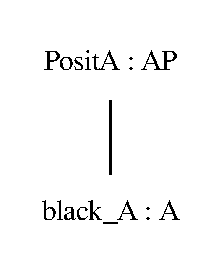
\includegraphics[scale=0.75]{figure/black_cats/black_AP_gf.eps}}
    \caption{The available GF trees on the word ``black'' after the first iteration}\label{fig:black iter 1}
\end{figure}

% A picture like 3.2, but with both the subtrees above attached to the word "black_A"

After having processed the children of ``cat'', the \ac{UD} tree annotated with \ac{GF} trees looks like in \autoref{fig:children_nested_compact}.
\begin{figure}[H]
    \centering
    %% the black cat
    \setlength{\unitlength}{0.2mm}
    \begin{dependency}
        % TODO: Maybe don't center each line here
        \begin{deptext}[column sep=0.4cm]
              the\_Det : Det \& black\_A : A \& cat\_N : N \\
            \& PositA black\_A : AP \&  \\
        \end{deptext}
        \depedge{3}{1}{det}
        \depedge{3}{2}{amod}
        \deproot{3}{root}
    \end{dependency} \\
    \caption{An overview of the nested tree, after having processed both the dependent words ``the'' and ``black''.}
    \label{fig:children_nested_compact}
\end{figure}

Now that we are done with all the children of ``cat'', we can start processing it. We have \lstinline|cat_N : N|.

\begin{figure}[H]
    \centering
    \subcaptionbox{``cat'' : N}
        {
\includegraphics[scale=0.75]{figure/black_cats/cat_N_gf.eps}}
    \caption{The available GF trees on the word ``cat'' before the first iteration}\label{fig:cat iter 0}
\end{figure}

Looking through all the functions, only \lstinline|UseN : N -> CN ; head| takes an N as an argument, so that's the one that's applied, giving us \lstinline|UseN cat_N : CN|. Now we have the trees in \autoref{fig:cat iter 1}
% \begin{lstlisting}
%     cat_N : N
%     UseN cat_N : CN
% \end{lstlisting}

\begin{figure}[H]
    \centering
    \subcaptionbox{``cat'' as a noun : N}[0.4\textwidth]
        {
\includegraphics[scale=0.75]{figure/black_cats/cat_N_gf.eps}}
    \subcaptionbox{``cat'' as a common noun: CN}[0.4\textwidth]
        {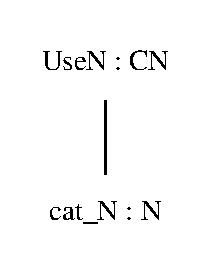
\includegraphics[scale=0.75]{figure/black_cats/cat_CN_gf.eps}}
    \caption{The available GF trees on the word ``cat'' after the first iteration}\label{fig:cat iter 1}
\end{figure}

In the next iteration we have a \lstinline|CN| available and can apply either of the functions
\begin{lstlisting}
    DetCN : Det -> CN -> NP ; det head
    ModCN : AP -> CN -> CN  ; amod head
\end{lstlisting}
Let us verify that these are possible to apply: For \lstinline|DetCN| we need a tree of type $Det$ with the $det$ \ac{UD} label for the relation and indeed, the word ``the'' has the $det$ label on the relation to ``cat'' and we have the tree \lstinline|the_Det : Det| available on ``the''. Secondly we need a $CN$ at the head and since our current head is ``cat'' and we have \lstinline|UseN cat_N : CN|, that fits perfectly giving us \lstinline|DetCN the_Det (UseN cat_N) : NP|. With similar reasoning for \lstinline{ModCN}, we have ``black'' with \ac{UD}-label $amod$ and one of the available trees for ``black'' is \lstinline|PositA black_A : AP| which has the correct category, which allows us to construct \lstinline|ModCN (PositA black_A) (UseN cat_N) : CN|. After this we have the trees in \autoref{fig:cat iter 2}

\begin{figure}[H]
    \centering
    \subcaptionbox{cat : N\label{cat_N}}
        {
\includegraphics[scale=0.75]{figure/black_cats/cat_N_gf.eps}}
    \subcaptionbox{cat : CN\label{cat_CN}}
        {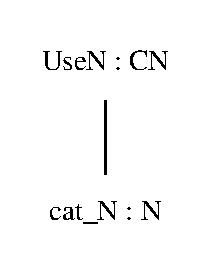
\includegraphics[scale=0.75]{figure/black_cats/cat_CN_gf.eps}}
    \subcaptionbox{the cat : NP\label{the_cat_NP}}
        {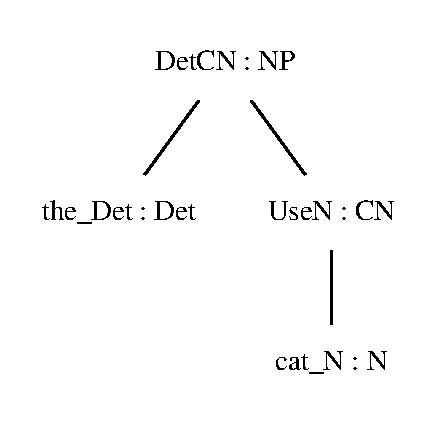
\includegraphics[scale=0.75]{figure/black_cats/the_cat_NP_gf.eps}}
    \subcaptionbox{black cat : CN\label{black_cat_CN}}
        {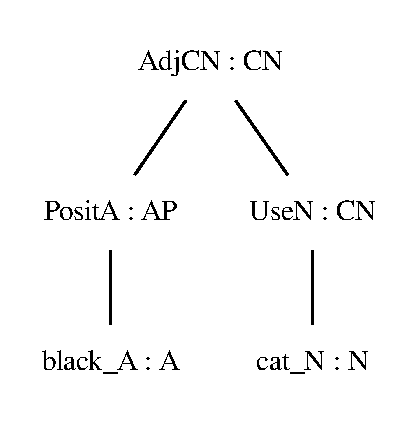
\includegraphics[scale=0.75]{figure/black_cats/black_cat_CN_gf.eps}}
    \caption{The four available trees on the word ``cat'' after the second iteration.}\label{fig:cat iter 2}
\end{figure}

After this iteration we have two trees on ``cat'' which both have the same category $CN$, namely
\begin{lstlisting}
    UseN cat_N : CN
    ModCN (PositA black_A) (UseN cat_N) : CN
\end{lstlisting}
and one of them is a strict superset of the other when it comes to words covered, the first only covers ``cat'' while the second covers both ``black'' and ``cat''. This means we can prune the redundant tree \lstinline{UseN cat_N}.


After this pruning, the available trees on the ``cat'' node can be seen in  \autoref{fig:cat iter 2 pruned}.
\begin{figure}[H]
    \centering
    \subcaptionbox{cat\label{ci2p:cat_N}}
        {
\includegraphics[scale=0.7]{figure/black_cats/cat_N_gf.eps}}
    \subcaptionbox{the cat\label{ci2p:the_cat_NP}}
        {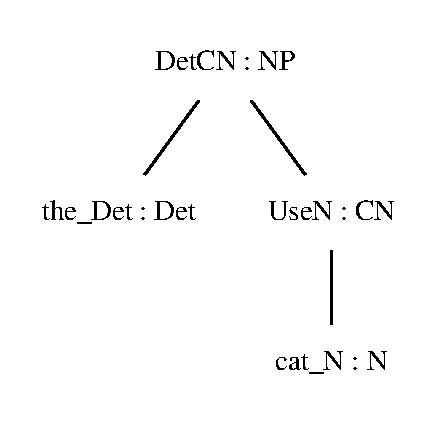
\includegraphics[scale=0.7]{figure/black_cats/the_cat_NP_gf.eps}}
    \subcaptionbox{black cat\label{ci2p:black_cat_CN}}
        {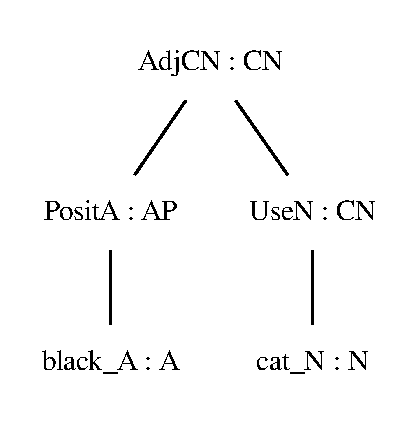
\includegraphics[scale=0.7]{figure/black_cats/black_cat_CN_gf.eps}}
    \caption{The three available trees on the word ``cat'' after the second iteration after pruning. Tree (b) will not be a subtree of the final tree.}\label{fig:cat iter 2 pruned}
\end{figure}
% \begin{lstlisting}
%     cat_N : N
%     DetCN the_Det (UseN cat_N) : NP
%     ModCN (PositA black_A) (UseN cat_N) : CN
% \end{lstlisting}
After this step, one function is still possible to apply, namely $DetCN$, which can be applied to our new $CN$ together with \lstinline{the_Det} like before, giving us the new tree
\begin{lstlisting}
    DetCN the_Det (ModCN (PositA black_A) (UseN cat_N)) : NP
\end{lstlisting}

\begin{figure}
    \centering
    \subcaptionbox{cat : N\label{ci3:cat_N}}
        {
\includegraphics[scale=0.6]{figure/black_cats/cat_N_gf.eps}}\\
    \subcaptionbox{the cat : NP\label{ci3:the_cat_NP}}
        {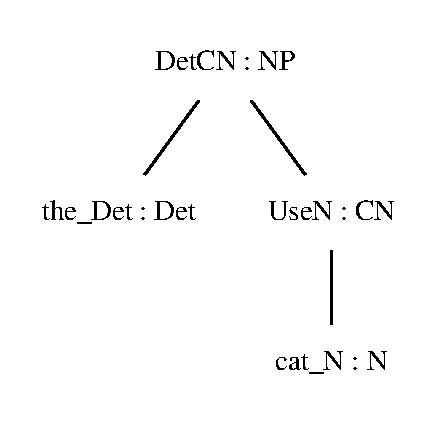
\includegraphics[scale=0.6]{figure/black_cats/the_cat_NP_gf.eps}}
    \subcaptionbox{black cat : CN\label{ci3:black_cat_CN}}
        {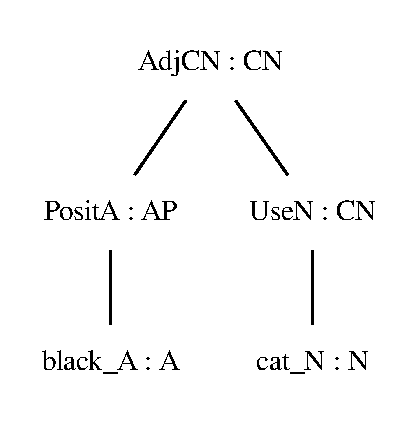
\includegraphics[scale=0.6]{figure/black_cats/black_cat_CN_gf.eps}}
    \subcaptionbox{the black cat : NP\label{ci3:the_black_cat_NP}}
        {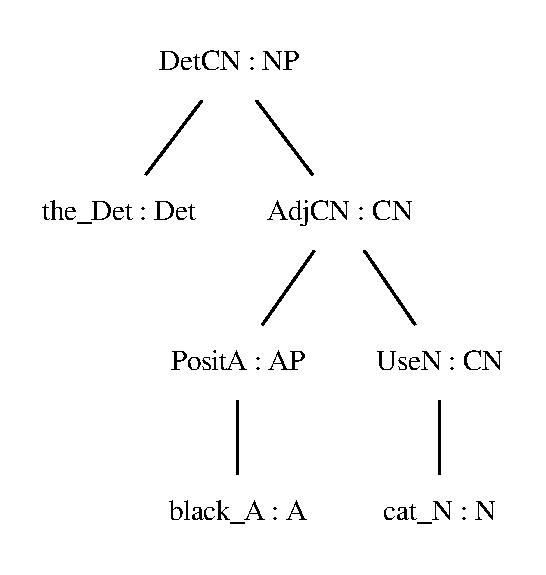
\includegraphics[scale=0.6]{figure/black_cats/the_black_cat_NP_gf.eps}}
    \caption{The four available trees on the word ``cat'' after the third iteration \emph{before} pruning. Trees (a) and (c) are both subtrees of the final tree (d), while tree (b) is not a subtree of (d), because it connects ``the'' directly to ``cat'' ignoring the adjective ``black''.}\label{fig:cat iter 3}
\end{figure}


and like before, we get multiple trees of the same category, this time of type $NP$, once again allowing us to prune the less covering tree.
\begin{lstlisting}
    DetCN the_Det (UseN cat_N) : NP
\end{lstlisting}

After this no more functions can be applied at the ``cat'' node, giving us a final set of cat trees as can be seen in \autoref{fig:cat iter 3 pruned}.
% \begin{lstlisting}
%     cat_N : N
%     ModCN (PositA black_A) (UseN cat_N) : CN
%     DetCN the_Det (ModCN (PositA black_A) (UseN cat_N)) : NP
% \end{lstlisting}

\begin{figure}[H]
    \centering
    \subcaptionbox{cat : N\label{ci3p:cat_N}}
        {
\includegraphics[scale=0.7]{figure/black_cats/cat_N_gf.eps}}
    \subcaptionbox{black cat : CN\label{ci3p:black_cat_CN}}
        {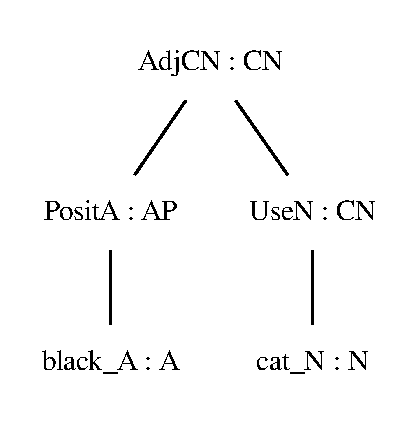
\includegraphics[scale=0.7]{figure/black_cats/black_cat_CN_gf.eps}}
    \subcaptionbox{the black cat : NP\label{ci3p:the_black_cat_NP}}
        {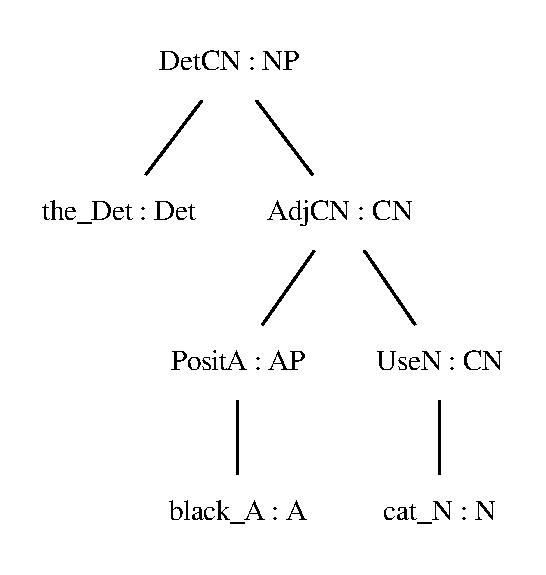
\includegraphics[scale=0.7]{figure/black_cats/the_black_cat_NP_gf.eps}}
    \caption{The three available trees on the word ``cat'' after the third iteration \emph{after} pruning. Trees (a) and (b) are both subtrees of the final tree (c).}\label{fig:cat iter 3 pruned}
\end{figure}

Now finally we have a complete tree which contains all of the words of the phrase, so we will choose the tree in \autoref{ci3p:the_black_cat_NP} as the final tree.

In the end, the data structure used in the calculation will look like in \autoref{fig:final nested tree} or \autoref{fig:final_nested_compact}, with the \ac{UD} structure outside which we traverse in order to find which parts can be connected and in each node of this tree a list of the \ac{GF} trees that are possible to construct using the words in the local \ac{UD} subtree, while conforming to the \ac{UD} labels. In this case, the word ``the'' has one \ac{GF} tree, the word ``black'' has two possible trees and the word ``cat'', which depends on the words ``the'' and ``black'' has four possible trees.

\begin{figure}[H]
    \centering
    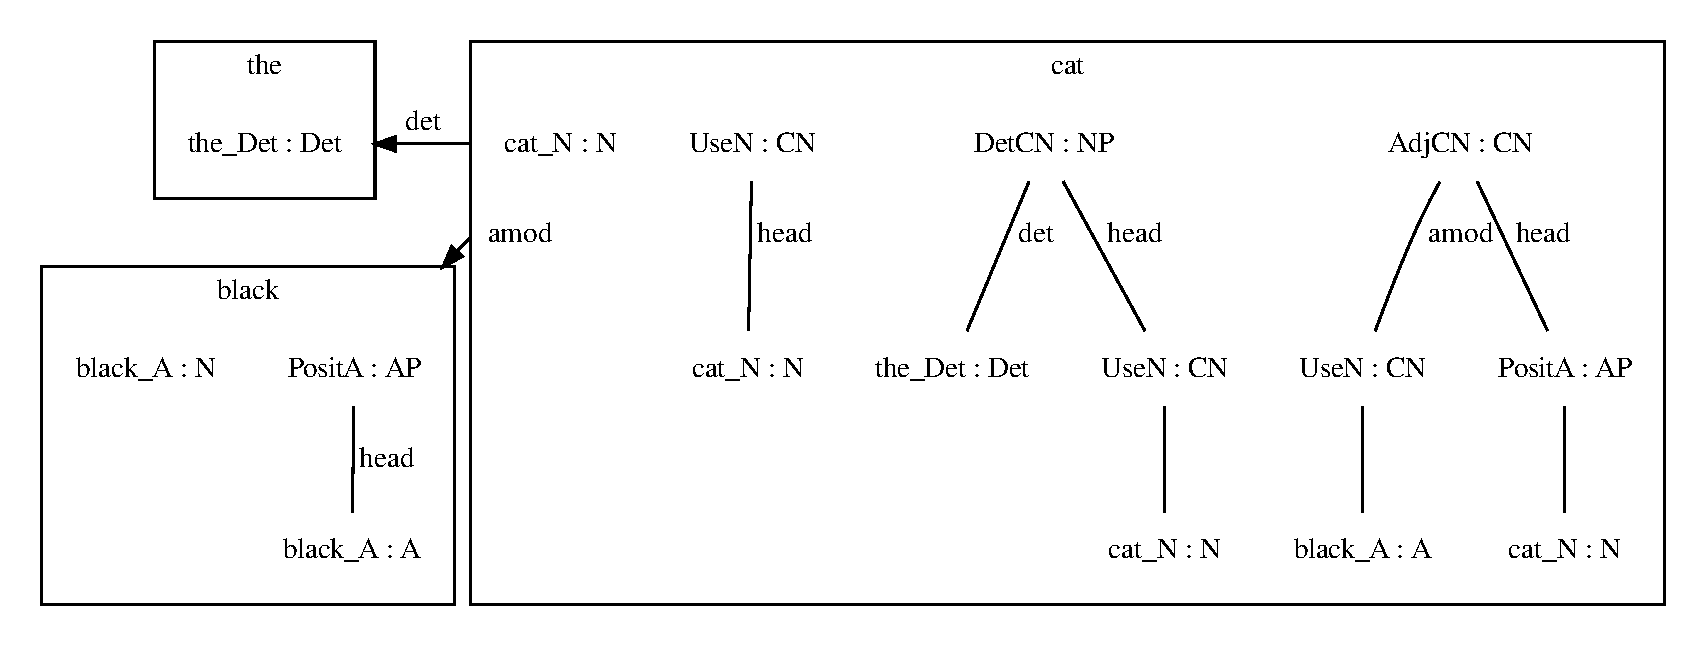
\includegraphics[width=0.7\textwidth]{figure/black_cats/the_black_cat_graph}
    \caption{An overview of the nested tree, with the UD structure outside and a list of GF-trees at each node}\label{fig:final nested tree}
\end{figure}

\begin{figure}[H]
    \centering
    %% the black cat
    \setlength{\unitlength}{0.2mm}
    \begin{dependency}
        % TODO: Maybe don't center each line here
        \begin{deptext}[column sep=0.4cm]
              the\_Det : Det \& black\_A : A \& cat\_N : N \\
            \& PositA black\_A : AP \& UseN cat\_N : CN \\
            \& \& DetCN the\_Det (UseN cat\_N) : NP \\
            \& \& AdjCN (PositA black\_A) (UseN cat\_N) : CN \\
        \end{deptext}
        \depedge{3}{1}{det}
        \depedge{3}{2}{amod}
        \deproot{3}{root}
    \end{dependency} \\
    \caption{An overview of the nested tree, with the UD structure outside and a list of GF-trees at each node.}
    \label{fig:final_nested_compact}
\end{figure}

% \FloatBarrier
% \clearpage
\subsection{Multiple possible GF trees of the same category}
\label{sec:multiple_trees}

In this simple example, we arrived at a state with intermediate trees that had the same type, and one was a strict subset of the other (``cat'' and ``black cat''). In a case like that, the old algorithm prunes away the smaller of the trees and continues on to the next iteration.

However, in a different grammar, we might very well end up with several trees that are of the same type, but not subsets of each other. This is the case for numerals in \ac{GF} standard library, where the trees for numbers like ``eight'', ``eighteen'' and ``eighty'' formed by applying different functions to the underlying digit called \texttt{n8}. Figure \ref{fig:eight} shows an example.

Due to the implementation of the \ac{GF} grammar, all of the strings ``eight'', ``eighteen'' and ``eighty'' are included in the inflection table of \texttt{n8}. This means that if the input contains any of these words, it matches the abstract syntax function \texttt{n8}, and then the next steps of the algorithm will start applying all possible functions to it. And since all of these functions are parallel alternatives, the results cannot be pruned like ``cat'' and ``black cat''. At the final step, when ud2gf is forced to present the user with only one alternative, the algorithm just picks the first tree from the intermediate list. This means that sometimes the results containing numerals are simply wrong: ``I have eight cats'' might become ``I have eighteen cats''.

To compensate for this issue, one can disable the potentially ambiguous functions using \verb|#disable| and use \verb|#auxfun| macros to ensure that all the relevant information is taken into consideration when deciding which trees are valid translations.

% \clearpage
\begin{figure}[t]
    \centering
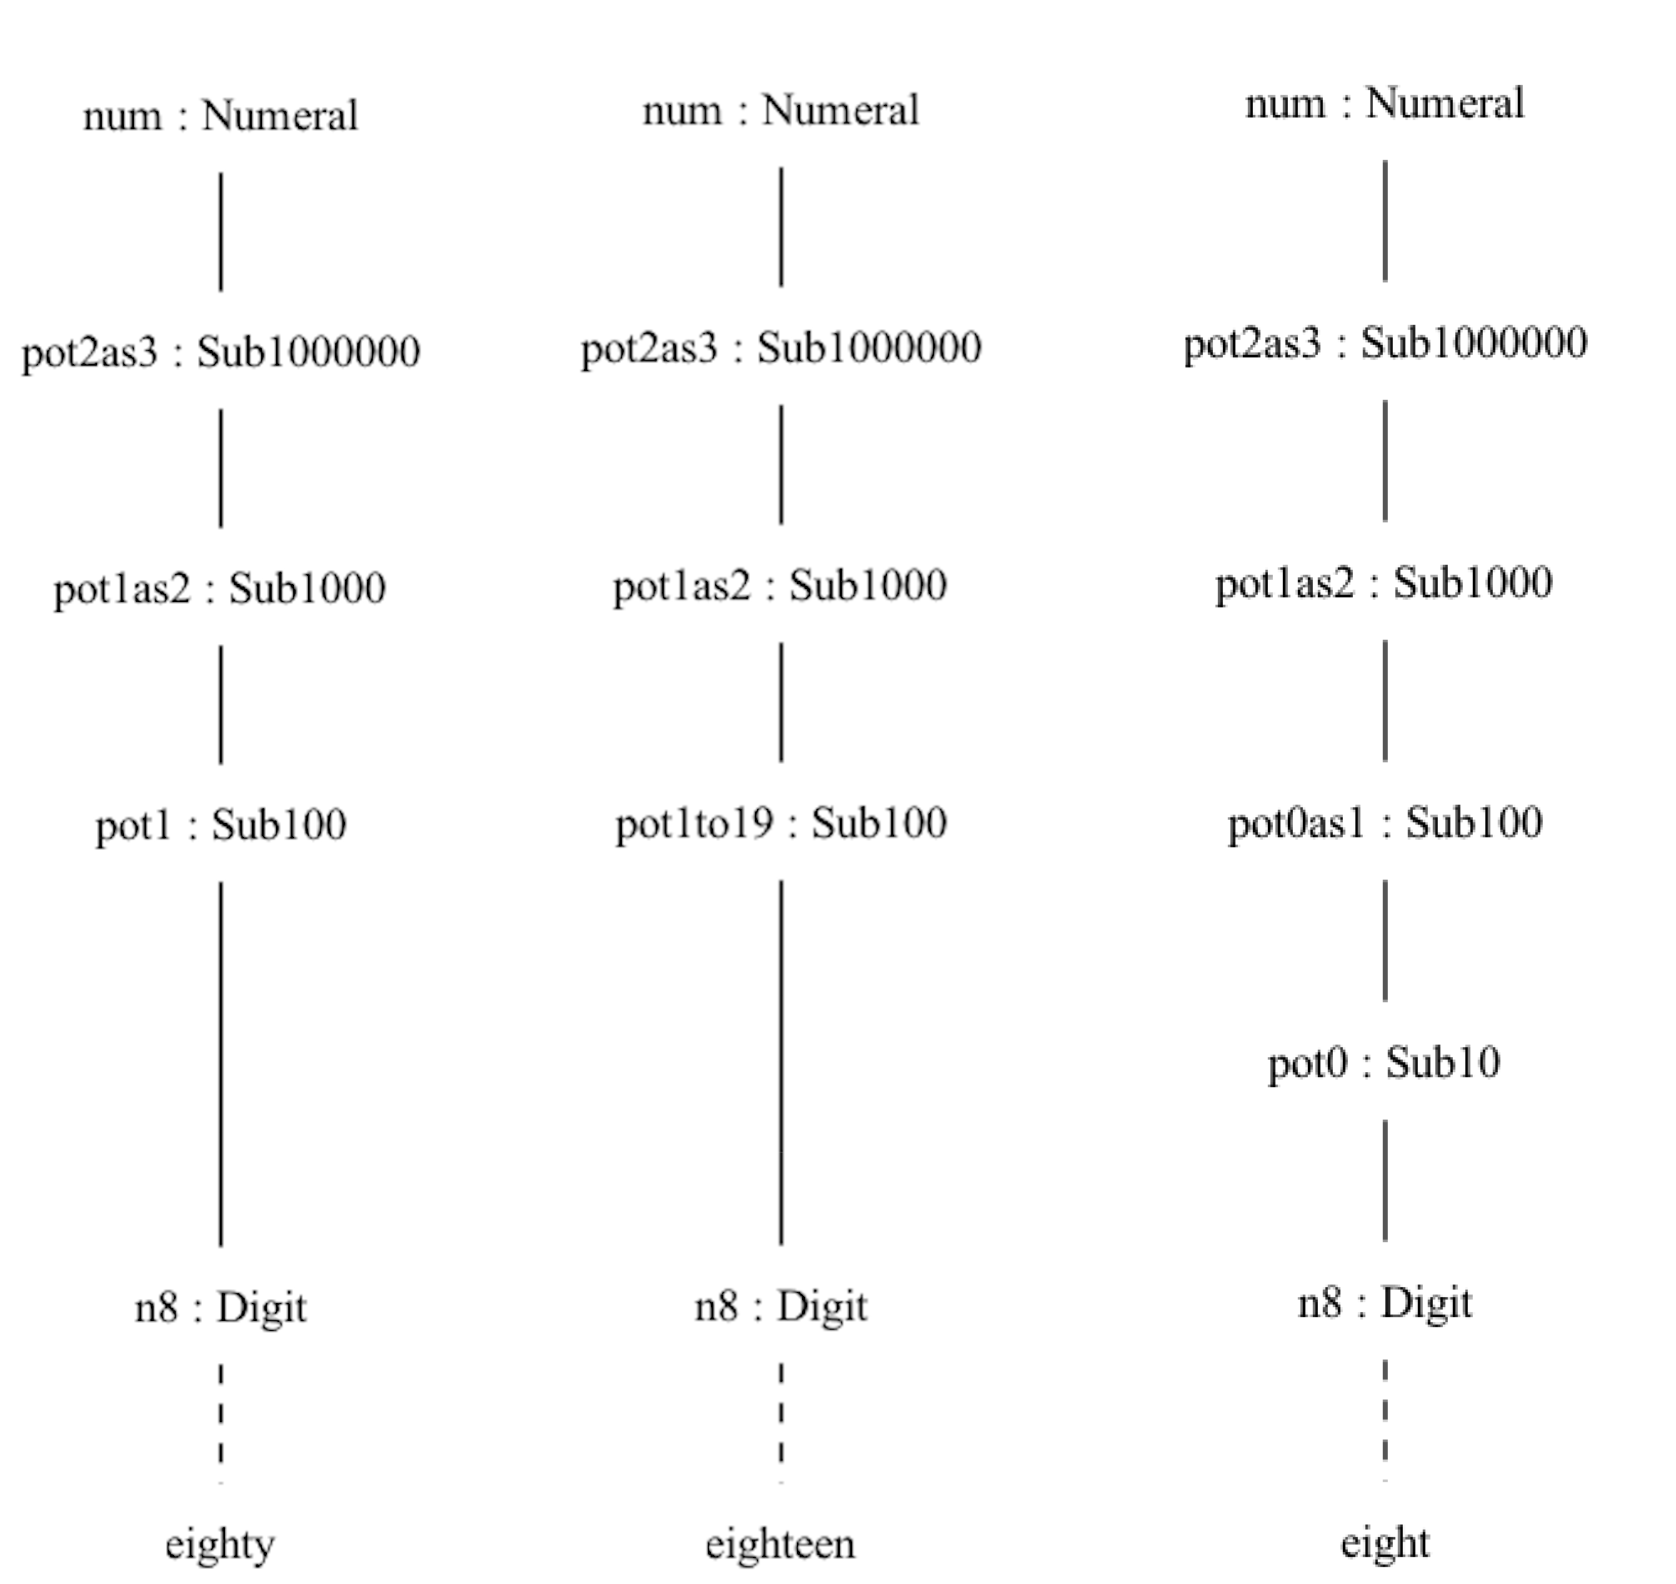
\includegraphics[scale=0.5]{figure/eight_eighteen_eighty.png}
    \caption{Three GF trees formed of the digit \texttt{n8}}
    \label{fig:eight}
\end{figure}

\section{Differences between versions}

% Each node in the UD tree corresponds to a word.

As explained in \autoref{sec:overview-of-algorithm}, the algorithm works as follows.
For each word, we try to apply all possible functions that match in both type and dependency label against the current head and a selection of children. As a result, we may get zero or more new trees for the given word.
Then we want to check if these new trees can, in turn, become the head argument for new function applications.
In the old algorithm, we check with \emph{all} the available trees for that word against each available function.

%After we have applied all possible functions and

%want to check if that

This means that all the trees that were possible to construct in the previous iteration are still possible to construct, so we will construct them again and will need to remove the duplicates afterwards.




% The new algorithm
\chapter{The new algorithm}

% TODO: 60 characters max in verbatim

In the new algorithm (version 3), we make two main improvements:

% \todo[inline]{Describe the pseudocode on a higher level, so the user don't need to read them}

\section{First improvement: faster keepTrying}

The first modification was to a function called \texttt{keepTrying}, which works with a word (the current head) in the UD tree and keeps trying to build new GF trees for that word based on the currently existing GF trees for the word and for its direct dependents, until no new trees can be built.

Before the improvement, pseudo-code of the algorithm would look roughly like this:
\begin{verbatim}
1. newTrees <- allFunsLocal(treesAtCurrentHead, childTrees)
2. combined <- deduplicate(treesAtCurrentHead ++ newTrees)
3. If combined != treesAtHead:
4.   treesAtHead <- combined
5.   Go to 1.
\end{verbatim}

Here, the function \texttt{allFunsLocal} (explained more in \autoref{sect:allFunsLocal}) tries to apply all possible GF functions to each of the trees at the current head. If the GF function that we try to apply takes more than one argument, then we choose that many trees from the dependents that the current tree has not used yet.

% In other words, we combine the new trees with the old trees in one big list which are reused for the next iteration.
%
% For each tree at the current head of the UD tree:
%     Apply all matching functions on the current tree, together with
%     some choice of trees from dependents that have so far not been
%     used by that tree, and add the result to the list of trees

This had the issue that the same trees were calculated many times just to be immediately thrown away. To solve this, we only calculate new trees based on trees we have not seen before at the current head of the UD tree:

\begin{verbatim}
1. newTrees <- treesAtCurrentHead
2. newTrees <- Apply all matching functions on each of newTrees, 
               together with a choice of unused 
3. treesAtCurrentHead += newTrees
4. if notEmpty(newTrees): goto 2
5. Deduplicate the list of trees
\end{verbatim}

In the first version, we only have one shared list of all the trees, both old and new trees mixed together. This means that the old trees will be used in every single iteration and time after time generate the same new trees. This produces a lot of duplicates that needs to be removed. In the new algorithm, we only generate based on the newest trees from the previous iteration, which eliminates these duplicates.

Since all previous trees were re-generated in each iteration, the old version was $O(n^2T)$ while the new version is $O(nT)$, where $n$ is the number of iterations (which is equal to the max depth of the tree) and $T$ is the number of possible trees at each level.

% Next line was first attempt at the above:
% The first improvement is that when new trees have been constructed by applying functions, we only use these new trees in the next iteration instead of putting both the old trees and the new trees in a shared list. This is because all the the trees that were possible to construct directly from the old trees have already been constructed, so there's no need to include them in the next iteration.

% WONTFIX: \todo[inline]{bild}

\section{Second improvement: faster allFunsLocal} \label{sect:allFunsLocal}

The second modification was to a function called \texttt{allFunsLocal}, which was responsible for finding all the possible combinations of functions and arguments at the current location in the UD tree that satisfy the constraints defined by the annotations. For example, for the function

\begin{verbatim}
#fun DetCN  : Det -> CN -> NP ; det  head
\end{verbatim}

the first argument needs to come from a child with UD dependency annotation \texttt{det} and be a GF tree with category \texttt{Det} and the second argument needs to be at the current local head of the UD tree and have a GF category of \texttt{CN}.

The old algorithm did this by first listing all possible choices of the previously generated trees for the head and each direct child of the current node and then trying each function for each of those choices. The new algorithm instead starts with each individual function and then only checks choices that could possibly match that function and stops as soon as it has determined that a match is impossible.

Below is pseudocode for the old algorithm for allFunsLocal:

Given the following variables:
\begin{verbatim}
headNode = A local UD head node with a list of possible GF trees
childNodes = A list of UD child nodes each with a list of
             possible GF trees
gfFunctions = A list of all GF functions that we have available
              and their metadata
\end{verbatim}

% 1. Generate all possible combinations of a GF tree from headNode and a GF tree from each of childNodes
% 2. For each

% TODO: Overfull hboxes
The algorithm looks as follows
\begin{verbatim}
1. For each gfFunction: f
2.   For each gf tree in headNode: headTree
3.     filteredChildNodes <- Filter out which childNodes have
                             not already been used by headTree
4.     childCombos <- Generate a list of all combinations, where
                      we select one GF tree from each element in
                      filteredChildNodes
5.     For each childCombo:
6.       For each argument of the function f: arg
7.         Select one element from childCombo or headTree which
             has not been used yet and which matches the required
             UD label and GF category
8.       Generate a list of all valid ways to select one valid
           childNode for each fun arg
\end{verbatim}

This algorithm can also be expressed in terms of a sequence of choices:
\begin{verbatim}
1. f <- Choose a gfFunction
2. headTree <- Choose a gf tree in headNode
3. childCombo <- For each childNode not already used by headTree:
4.     Choose a GF tree from the child node
5. For each argument of the function f: arg
6.   Select one element from childCombo or headTree which has not
       been used yet and which matches the required UD label and
       GF category
7. Generate a list of all valid ways to select one valid
       childNode for each fun arg
\end{verbatim}

This algorithm is unfortunately exponential. More precisely:

If we have $f$ functions, each taking $a$ arguments and
if the headNode contains $h$ gf-trees
and we have $c$ child-nodes, each containing $t$ gf-trees
and each argument matches $m$ values from childCombo, we get an algorithmic complexity of:

% \todo[inline]{TODO: better alternative to $m$ which reflects reality better. $m$ cannot possibly be a constant and will often vary between 0 and 1}

$$
O(f h t^c (ac+m^a))
$$

We can see that the complexity is exponential with respect to the number of child-nodes, with a base proportional to how many GF trees each of those child-nodes have. The complexity is also exponential with the number of arguments, but this has less of an impact since GF functions always have a fixed number of arguments, unlike UD trees, where a node can have an unlimited number of children, e.g. in conjunctions.

% \todo[inline]{TODO: Appendix with the actual source}

In addition to having an exponential complexity, this also produces duplicate trees. To see this we need to go through an example.

Let's say we have one function \verb|DetCN : Det -> CN -> NP ; det head| which takes two arguments and a UD tree with a head node \emph{cat} and two children \emph{the} and \emph{black}: (See \autoref{fig:final nested tree})

Now, if we were to apply this algorithm, we would generate these lists of combinations:
\begin{verbatim}
       cat ; head      | the ; det     | black ; amod
       cat_N      : N  | the_Det : Det | PositA black_A : AP
       UseN cat_N : CN |               | black_A        : A
\end{verbatim}

\begin{verbatim}
    1. cat_N      : N , the_Det : Det, black_A        : A
    2. cat_N      : N , the_Det : Det, PositA black_A : AP
    3. UseN cat_N : CN, the_Det : Det, black_A        : A
    4. UseN cat_N : CN, the_Det : Det, PositA black_A : AP
\end{verbatim}

If we now check where the function can be applied, we can see that both 3 and 4 matches,
but in both cases they produce the same tree:
\begin{verbatim}
    DetCN the_Det (UseN cat_N)
\end{verbatim}
because the only difference is in the unused child node \verb|black|.

In order to solve both the issue of poor complexity and producing duplicates, in the new algorithm, we delay the selection of tree until the latest possible moment.


% Note: still exponential if many matching (equivalent) children. These will still be thrown away in the next step anyways


\begin{verbatim}
1. For each gfFunction: f
2.   headArg <- Find the argument of f with label "head"
3.   For each headTree in headNode.trees where
              headTree.cat == headArg.cat:
4.     filteredChildNodes <- Filter out which childNodes have not
                             already been used by headTree
5.     For each non-head argument of f: arg
6.       For each node in filteredChildNodes, where
                  node.label == arg.label: childTree
7.         return each tree where childTree.cat == arg.cat
8.     Construct a list of trees using f and each of the valid
         child-trees (if any)
\end{verbatim}

We can also express the same thing in terms of a sequence of choices:

\begin{verbatim}
1. Make a list of trees from every possible combination of
   choices below:
2.   f <- Choose a function from gfFunctions
3.   headArg <- Find the argument of f with label "head"
4.   headTree <- Choose a tree in headNode where 
                     headTree.cat == headArg.cat:
5.   filteredChildNodes <- Filter out the childNodes that have not 
                               already been used by headTree
6.   childArgTrees <- For each non-head argument of f: arg
7.       childNode <- Choose a node in filteredChildNodes, where 
                          node.label == arg.label:
8.       Choose a tree in childNode where childTree.cat == arg.cat
9.   Construct a tree using f, headTree and each of the childArgTrees
\end{verbatim}

% Solved: \todo[inline]{Overflow}

Now $h_m$ is the number of trees in the head node which \emph{matches} the head argument instead of every tree in the head node.

$$
O(f h_m (c+m)^a)
$$

The complexity here is in most cases very close to just the number of trees we are generating with only a linear overhead. % \todo{is this true?}

Because we delayed the choice of tree until we know we need it we are no longer generating duplicate trees.
We also have the ability to stop early, as soon as one of the arguments are impossible to satisfy, we don't need to check the rest.

One possible inefficiency that remains is that if many children have the same label and category as each other we will
generate every possible tree that uses these and then in a later stage filter out so we only have a single tree with that specific category. It might be possible to keep track of these so we don't needlessly produce redundant trees that will soon be thrown away anyways. 
Another possible solution would be to have ordering constraints, so that with the otherwise equivalent children, they are forced to be used in a specific order. This would be especially relevant with coordinate structures (see also \autoref{sect:flex}), in which each child has the same category and dependency label and the ordering is important.

% however it's probably not exponential in practice (?)
% \todo[inline]{Fix this!}

% Most of the time when this happens we would like for 


% Another issue that has not been dealt with is infinite loops


% The debugger
\chapter{Debugger}

\section{Problem description}

An issue that was encountered when trying to write annotations for \texttt{ud2gf} is that sometimes it can be difficult to figure out why a rule does not fire.

The goal of the debugger project is to automatically give an explanation of why a rule (function label description) doesn't match.


% TODO: Better example

% Let's say we have the function $DetCN : Det -> CN -> NP ; det head$ and want to know why it wasn't used. We would call the tool with the argument \verb|dbg="DetCN 3 5"| and we would get out an explantation

Let's say we have the sentence ``colorless green ideas sleep furiously'' and believe that the function \verb|DetCN : Det -> CN -> NP ; det head| should be applied to ``green'' and ``ideas'' respectively, but it doesn't seem to be
used for some reason. Then we would call the \texttt{ud2gf} tool with either \verb|dbg="DetCN 2 3"| or \verb|dbg="DetCN green ideas"| and the debugger would give back one of a list of reasons to what prevented it from being applied:

\begin{itemize}
    \item The function has been manually disabled.
    \item The function does not exist.
    \item There are multiple definitions of the function.
    \item The wrong number of arguments was given to the debugger (meta-error).
    \item The requested indices are not found within the UD tree.
    \item The non-head arguments are not direct children of the head argument.
    \item The non-head arguments have labels that don't match the labels within the UD-tree.
    \item Required features are missing for some of the arguments.
    \item No trees with the required category could be found for some of the arguments.
    \item The function was possible to apply, but was pruned away because a different tree with the same category had higher priority.
\end{itemize}

If a word exist multiple times in the sentence, you need to use the number form, otherwise you will get an ``Ambiguous word'' error. In order to see the index number of a word you can either look at the conllu file\footnote{Conllu is the standard file format for UD trees.} directly or run \verb|ud2gf| with the \verb|ud| or \verb|ut| argument.


\section{Implementation}

The implementation is mostly a case of going through every step of the algorithm and seeing what can go wrong. Some of this process was simplified by the strong type system of Haskell, since it makes edge cases explicit, so in most cases we would get a type error if we missed handling a possible error.

In order to simplify the implementation and reduce code duplication, we first run the main algorithm to generate all possible GF trees in each node of the UD tree and use this result to check what goes wrong with the specific function we are interested in.

\section{Example}

Let's look at the phrase ``large portion of walls'', which in UD format looks like this:

\begin{center}
    \begin{dependency}
        \begin{deptext}[column sep=0.4cm]
              {\tt large}\&{\tt portion}\&{\tt of}\&{\tt walls}\\
            {\tt ADJ}\&{\tt NOUN}\&{\tt ADP}\&{\tt NOUN}\\
        \end{deptext}
        \depedge{2}{1}{amod}
        \depedge{2}{4}{nmod}
        \depedge{4}{3}{case}
        \deproot{2}{root}
    \end{dependency}
\end{center}
    
First we try to form a tree of words that are not in a head--dependent relation. The tool reports that \emph{large} is not a child of \emph{walls}, and suggests an actual child of \emph{walls} (i.e. \emph{of}) as a hint for the grammar writer.

\begin{lstlisting}
$ cat tests/examples/large_portion_of_walls.conllu | gf-ud ud2gf tests/grammars/Test Eng UDS no-backups dbg='AdjCN large walls'

Starting debug for AdjCN:
AdjCN : AP -> CN -> CN ; amod head
Error: Word number 1 ("large")  is not a child of 4 ("walls").
    Available children: [("3","of")]
\end{lstlisting}

Next, we ask the debugger about a correct attachment, but we try to apply a function of the wrong type. The debugger answers with ``Incompatible argument labels''.


\begin{lstlisting}
$ cat tests/examples/large_portion_of_walls.conllu | gf-ud ud2gf tests/grammars/Test Eng UDS no-backups dbg='DetCN large portion'

Starting debug for DetCN:
DetCN : Det -> CN -> NP ; det head
Attempting to build: DetCN large portion
Error: Incompatible argument labels:
 - For "large": Got amod expected det
\end{lstlisting}

Finally, if we debug a correct application, we get a step by step trace of how the tree is constructed.

\begin{lstlisting}
$ cat tests/examples/large_portion_of_walls.conllu | gf-ud ud2gf tests/grammars/Test Eng UDS no-backups dbg='AdjCN large portion'

Starting debug for AdjCN:
AdjCN : AP -> CN -> CN ; amod head
Attempting to build: AdjCN large portion

Argument "large" : AP ; amod:
  Found trees with correct category:
    - (PositA large_A) : AP

Argument "portion" : CN ; head:
  Found trees with correct category:
    - (AdvCN (UseN portion_N) (PrepNP of_Prep (DetCN_aPl (UseN wall_N)))) : CN
Trees using AdjCN found in devtree:
    (AdjCN (PositA large_A) (AdvCN (UseN portion_N) (PrepNP of_Prep (DetCN_aPl (UseN wall_N))))) : CN
Success!
\end{lstlisting}


% In this case the tree was successfully built, but pruned away because other trees had a higher priority. This typically means that you need to disable some functions and replace them with more specific functions to ensure that the desired functions are used.

% First the main algorithm is run and afterwards all the generated trees are searched, this can lead to some information being missing compared to actually tracing running the algorithm and detecting where where it goes wrong. However in practice it works well enough and it significantly simplifies the implementation, since the main algorithm doesn't need to be modified nor duplicated in order to implement the debugger.


% Macro flexibility
\chapter{Improving flexibility of macros}
\label{improving-flexibility-macros}

\todo[inline]{Explain the old macro system with an example. Q: Isn't that the section below already?}



\section{Explanation of the macro system}

% What are the limitations without macros?
% Most importantly: syncats. gf-ud assumes that every word is in a leaf, represented by a lexical gf-function. however, syncategorimatic words \todo{define?} (or functions?) come from the functions that are used to combine trees (what are those called?) and would be missing otherwise. E.g. "is" is syncategorimatic in gf for english, because there is no lexical function for copula, because not all languages use a word for copula. So we make up a lexical gf-function for "is", which is then combined with a made-up version of MkCl which is converted into the thing we need.
% This is terrible writing!

In order to overcome some limitations \todo{(which?)} of the conversion there is a system of macros. A macro is an imaginary GF function that will get converted into an expression of real GF functions after the conversion step of gf2ud is done.

% Syncats?

When one GF function corresponds to multiple different dependency labels, a macro can be used to disambiguate which one is meant without losing the information

Example from \cite{kolachina-ranta-2017}



% We noted in Section 2 that ud2gf has to deal with
% ambiguity, incompleteness, noise, and ungrammaticality. The basic algorithm of Section 3 takes
% none of these aspects into account. But it does
% contain what is needed for ambiguity: the list ts
% of previous trees at each node can also be used
% more generally for storing alternative trees. The
% “main” tree t is then compared and ranked together with these candidates. Ranking based on
% tree probabilities in previous GF treebanks, as in
% (Angelov, 2011), is readily available. But an even
% more important criterion is the node coverage of
% the tree. This means penalizing heavily those trees
% that don’t cover all nodes in the subtrees.
% This leads us to the problem of incompleteness:
% what happens if the application of all possible candidate functions and trees still does not lead to a
% tree covering all nodes? An important part of this
% problem is due to syncategorematic words. For
% instance, the copula in GF is usually introduced as
% a part of the linearization, and does not have a category or function of its own.6 To take the simplest
% possible example, consider the adjectival predication function and its linearization:
% fun UseAP : AP -> VP
% lin UseAP ap = \\agr => be agr ++ ap
% where the agreement feature of the verb phrase is
% passed to an auxiliary function be, which produces
% the correct form of the copula when the subject
% is added. The sentence the cat is black has the
% following tree obtained from UD:





\begin{verbatim}
#auxfun MkVPS_Perf have vp : Have -> VP -> VPS = MkVPS (TTAnt AAnter 
  TPres) PPos vp ; aux[Tense=Pres] head
\end{verbatim}

\section{Intro to macros}

% Motivate need for auxfuns and auxcats

GF trees are on a higher abstraction level than UD trees. In UD, every token is associated with a dependency label. In contrast, any production rule in a GF grammar may introduce new tokens. This difference complicates the mapping between the two formalisms.

When introducing the problem and its partial solution, \cite{kolachina-ranta-2017} name as examples copulas, negations, tense auxiliaries and infinitive marks. We reproduce their example of the English copula (the verb “to be”) and its treatment in \verb|ud2gf|.

Figures \ref{fig:gf_cute} and \ref{fig:ud_cute} show the difference between GF’s and UD’s treatment of copulas. In the UD tree, the copula has a category and a dependency label \verb|cop|. In the GF tree, there is no special category: the string “is” is introduced by the function \verb|UseComp : AP -> VP| rule, which makes an AP into a predicate.

% \begin{figure}
%     \centering
%     \includegraphics{}
%     \caption{Caption}
%     \label{fig:enter-label}
% \end{figure}

result from \verb+p -cat=Cl "this cat is small"  | vp -view=open -showfun+:

% Produced using: https://maryszmary.github.io/ud-annotatrix//standalone/annotator.html
% And pressing the printer icon to select latex

\begin{figure}
    \centering
    % \includegraphics{}
    \begin{dependency}
       \begin{deptext}[column sep=0.4cm]
             this \& cat \& is \& small \\
           {\tt DET}\&{\tt NOUN}\&{\tt AUX}\&{\tt ADJ}\\
       \end{deptext}
       \depedge{2}{1}{det}
       \depedge{4}{2}{nsubj}
       \depedge{4}{3}{cop}
    \end{dependency} \\
    \caption{The phrase ``This cat is small'' analysed as a UD tree}
    \label{fig:enter-label}
\end{figure}

As a solution, \verb|ud2gf| introduced the notion of \emph{auxiliary categories} and \emph{auxiliary functions} in the labels file. This consists of the following parts:
\begin{itemize}
    \item Auxiliary category for copula: \verb|Cop_ VERB lemma=be|
    \item Auxiliary function that recognises the auxiliary category: \\
           \verb|UseAP_ : Cop_ -> AP -> VP ; cop head|
    \item Rule to replace the auxiliary function with an actual GF function: \\
          \verb|UseAP_ cop ap = UseAP ap|
\end{itemize}

However, coordination was still a problem in \verb|ud2gf|. The auxiliary categories and functions were not expressive enough to transform a structure like ``the small, cute and fluffy cat'' from UD to GF.





\section{Intro to flexibility problem}

As an example of a phrase that can be difficult to convert using the old gf2ud, let us consider the adjectival phrase ``cute, fluffy and furry''
would be described in UD format as in Figures \ref{fig:ud_cute_text} and \ref{fig:ud_cute}.


\begin{figure}
    \begin{verbatim}
    1  cute  cute  ADJ  JJ  Degree=Pos  0  root  _  FUN=cute_A
    2  ,  ,  PUNCT  ,  _  3  punct  _  _
    3  fluffy  fluffy  ADJ  JJ  Degree=Pos  1  conj  _  FUN=fluffy_A
    4  and  and  CCONJ  CC  _  5  cc  _  FUN=and_Conj
    5  furry  furry  ADJ  JJ  Degree=Pos  1  conj  _  FUN=furry_A
    \end{verbatim}
    % \begin{tabular}{|c|c|c|c|c|c|c|c|c|c|}
    % \hline
    % 1 & cute & cute & ADJ & JJ & Degree\=Pos & 0 & root & \_ & FUN\=cute\_A \
    % \hline
    % 2 & , & , & PUNCT & , & \_ & 3 & punct & \_ & \_ \
    % \hline
    % 3 & fluffy & fluffy & ADJ & JJ & Degree\=Pos & 1 & conj & _ & FUN\=fluffy\_A \
    % \hline
    % 4 & and & and & CCONJ & CC & \_ & 5 & cc & \_ & FUN\=and\_Conj \
    % \hline
    % 5 & furry & furry & ADJ & JJ & Degree\=Pos & 1 & conj & \_ & FUN\=furry\_A \
    % \hline
    % \end{tabular}
    \caption{The phrase ``cute, fluffy and furry'' as a textual UD tree}
    \label{fig:ud_cute_text}
\end{figure}

\begin{figure}
    \centering
    % \begin{dependency}
  \begin{deptext}[column sep=0.4cm]
      cute \& , \& fluffy \& and \& furry \\
    {\tt ADJ}\&{\tt PUNCT}\&{\tt ADJ}\&{\tt CCONJ}\&{\tt ADJ} \\
  \end{deptext}
  \depedge{2}{1}{punct}
  \depedge{0}{2}{conj}
  \depedge{4}{3}{cc}
  \depedge{0}{4}{conj}
\end{dependency} \\
    % \includesvg{ud-annotatrix-corpus.svg}
    % 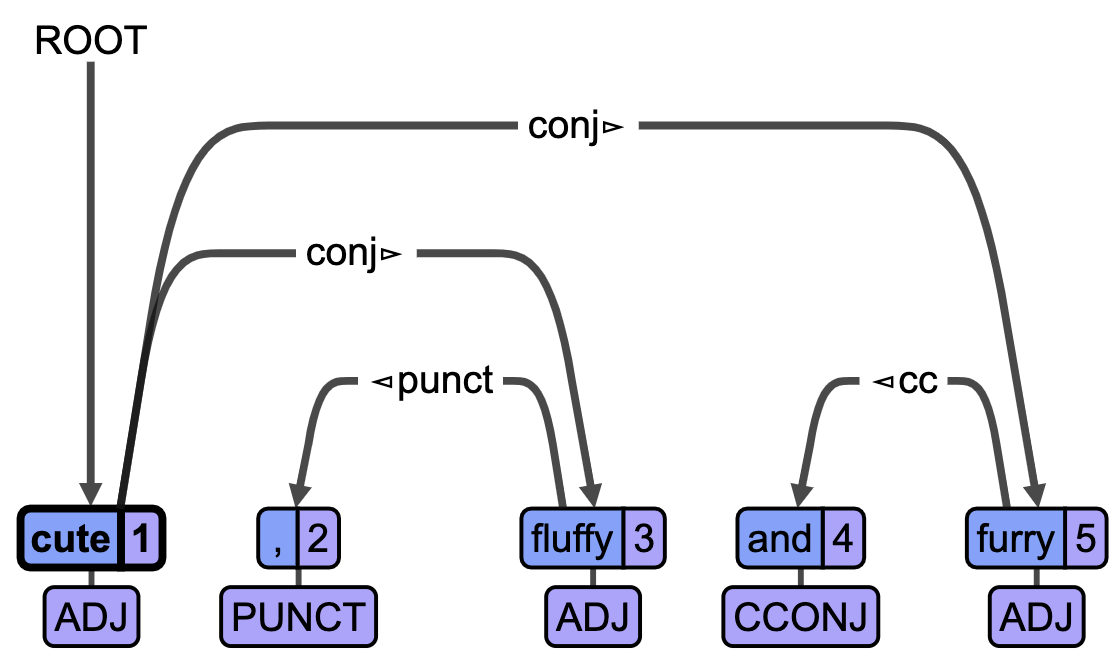
\includegraphics[width=0.7\textwidth]{figure/ud_cute.png}
    \begin{dependency}
        \begin{deptext}[column sep=0.4cm]
              cute \& , \& fluffy \& and \& furry \\
            {\tt ADJ}\&{\tt PUNCT}\&{\tt ADJ}\&{\tt CCONJ}\&{\tt ADJ}\\
        \end{deptext}
        \depedge{3}{2}{punct}
        \depedge{1}{3}{conj}
        \depedge{5}{4}{cc}
        \depedge{1}{5}{conj}
    \end{dependency} \\
    \caption{The phrase ``cute, fluffy and furry'' as a UD tree in graphical format}
    \label{fig:ud_cute}
\end{figure}
% \include{}

\begin{figure}
    \centering
    % \begin{dependency}
  \begin{deptext}[column sep=0.4cm]
      cute \& , \& fluffy \& and \& furry \\
    {\tt ADJ}\&{\tt PUNCT}\&{\tt ADJ}\&{\tt CCONJ}\&{\tt ADJ} \\
  \end{deptext}
  \depedge{2}{1}{punct}
  \depedge{0}{2}{conj}
  \depedge{4}{3}{cc}
  \depedge{0}{4}{conj}
\end{dependency} \\
    % \includesvg{ud-annotatrix-corpus.svg}
    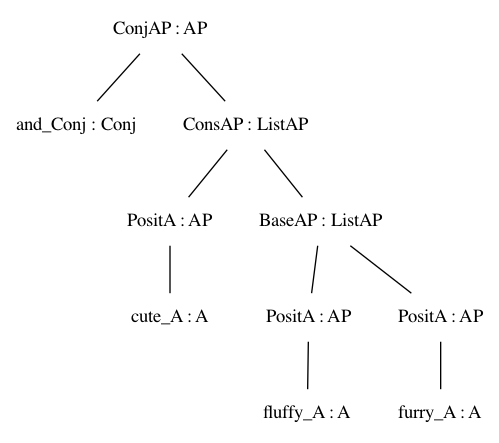
\includegraphics[width=0.7\textwidth]{figure/cute_gf.png}
    \caption{The phrase ``cute, fluffy and furry'' as a GF tree in graphical format. }
    \label{fig:gf_cute}
\end{figure}

The GF version of the same tree, shown in Figure \ref{fig:gf_cute}, would look like this:

\begin{verbatim}
ConjAP and_Conj (ConsAP (PositA cute_A)
                        (BaseAP (PositA fluffy_A) (PositA furry_A)))
\end{verbatim}
Here we can see that in UD, the word ``cute'' is in the root, while the conjunction ``and'' is at the bottom of the tree, while in GF the conjunction is a direct child of the root. This transformation can not be preformed by the simple single-layer transformations that are available in the current macro-system for labels files.



\section{Thing}

Most of the time the structure in UD trees are similar enough to allow a fairly direct translation.
There are however some difficult cases where the structure is significantly different in a way that was impossible to overcome using the old macro system.

One such example is when you have a series of conjunctions, for example the phrase:

  small, fluffy, furry and cute

In 

\section{Ideas for further improvements}

A more structured implementation of this could be to add (anonymous) records to the syntax of macros similar to the concrete syntax of GF. 

% RESULTS
% \chapter{Evaluation}
One method for evaluation is through synthetic experiments of generating random GF trees through GF's built-in functionality, then translating those to UD trees and then back to GF again. There are several different aspects that could be evaluated here:
\begin{itemize}
    \item Completeness: the ability to always get complete trees without needing to invent what GF2UD calls Backup GF functions, for when no functions in the GF grammar were possible to use to connect a subtree
    \item Accuracy: How well the tree matches the original after a roundtrip
    \item Performance: How fast the code runs
    \item Error analysis: Examine the cause of errors and issues
\end{itemize}

% 4. Evaluation
% - synthetic experiment: RGL -> UD -> RGL
%   - completeness - kan alltid få ett fullständigt träd
%   - accuracy
%   - performance
%   - error analysis



% CREATED BY DAVID FRISK, 2016
\chapter{Results}
% Describe you results. Use tables, diagrams etc. for illustration.

\section{Performance}

% Undersök varför inte alla meningar ger samma resultat
% Kör hela upto12eng och jämför diff för statistik och hitta mönster

% Idé: Scatter-plot av optimerad mot ooptimerad

The result of running different versions of the algorithm on the example file \texttt{upto12eng.conllu} using the example grammar \texttt{ShallowParse} in the gf-ud git repository can be seen in \autoref{fig:time-including-gc}. The full list of sentences included in the benchmark can be seen in \autoref{app:upto12}. All benchmarks were perfomed on a 2019 MacBook Pro, with a 2.3 GHz 8-Core Intel Core i9 CPU.

\begin{table}[]
    \centering
    \begin{tabular}{c|ccc}
Time (seconds) & Calculation & Garbage Collection & Total \\
\hline
Original code & 2m 58s 834ms & 24s 637ms & 3m 23s 471ms \\
Original code (fast GC) & 3m 1s 872ms & 20s 241ms & 3m 22s 113ms \\
fastKeepTrying & 26s 171ms & 14s 767ms & 40s 938ms \\
fastKeepTrying (fast GC) & 28s 631ms & 1s 705ms & 30s 336ms \\
fastAllFunsLocal & 3s 166ms & 14s 31ms & 17s 197ms \\
fastAllFunsLocal (fast GC) & 3s 203ms & 1s 253ms & 4s 456ms \\
Both improvements & 2s 687ms & 13s 922ms & 16s 609ms \\
Both improvements (fast GC) & 1s 253ms & 1s 253ms & 2s 506ms \\
    \end{tabular}
    \caption{The total run time for converting the file upto12eng.conllu, including garbage collection and startup time. The bars marked ``fast GC'' have increased initial heap size to 500Mb to reduce the number of unnecessary garbage collections, based on the experiments in \autoref{sect:gc-time}. TODO: Perform multiple measurements to reduce noise. Also, don't include milliseconds, when we don't have that precision. }
    \label{tab:time-with-gc}
\end{table}

In \autoref{fig:time-vs-time} we can see the speedup for each individual sentence. The improvement of the keepTrying function gives a close to linear speedup, while the speedup from the optimized version of allFunsLocal is much larger. The theoretical expected speedup from keepTrying is a quadratic factor that becomes a linear factor based on the depth of the resulting trees. This 
\begin{figure}
    \centering
    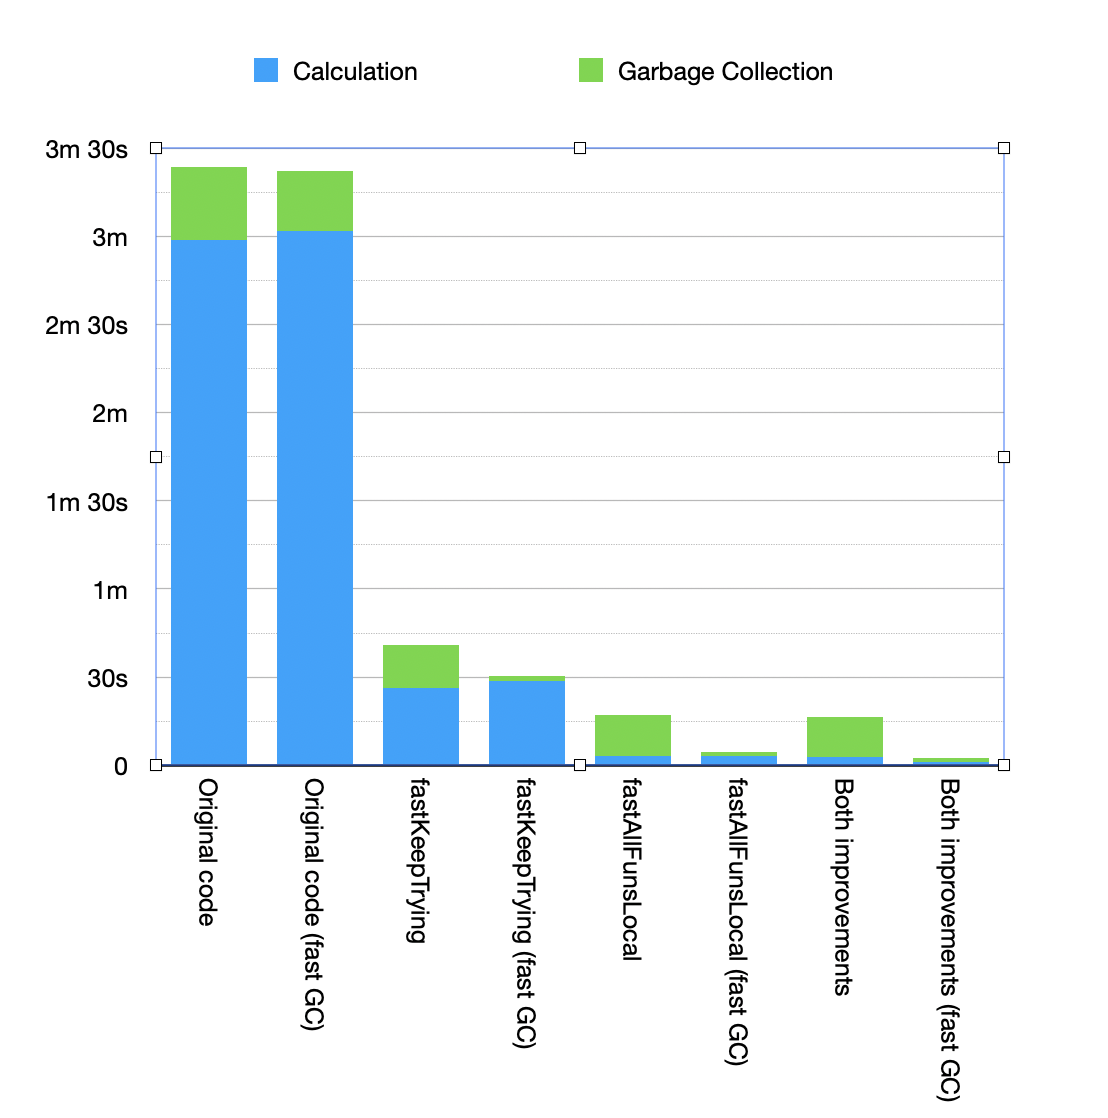
\includegraphics[scale=0.75]{thesis/figure/Time-including-GC.png}
    \caption{The total run time for converting the file upto12eng.conllu, including garbage collection and startup time. The bars marked ``fast GC'' have increased initial heap size to 500Mb to reduce the number of unnecessary garbage collections, based on the experiments in \autoref{sect:gc-time}. TODO: Perform multiple measurements to reduce noise.}
    \label{fig:time-including-gc}
\end{figure}

\begin{figure}
    \centering
    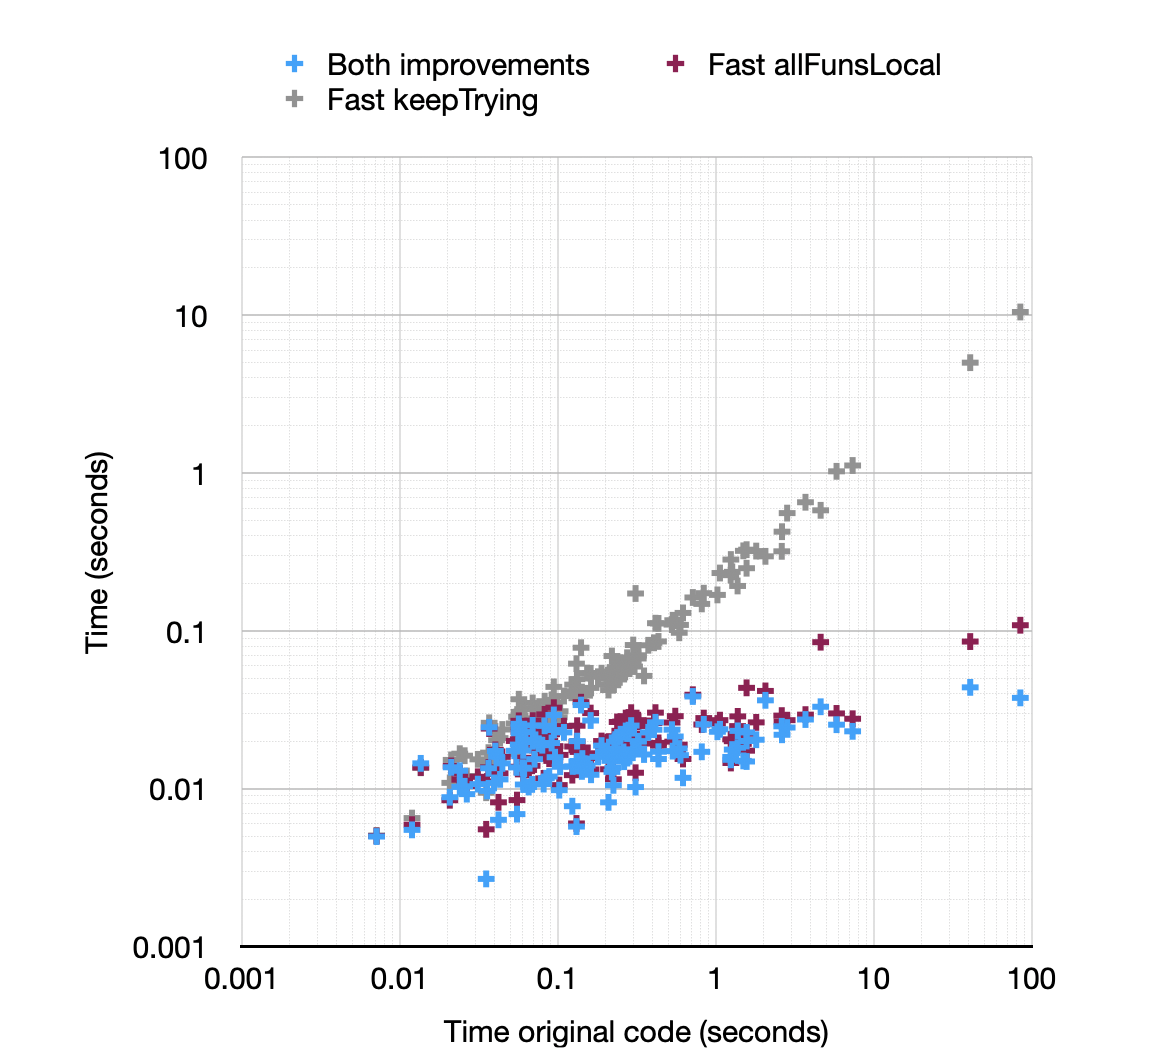
\includegraphics[scale=0.75]{thesis/figure/Time-against-time-plot.png}
    \caption{A log-log plot of time for each optimization against the time for the original algorithm. Each data point is the average time over several runs for a single sentence. The library Criterion\protect\footnotemark{} was used to perform the measurements.}
    \label{fig:time-vs-time}
\end{figure}

\footnotetext{http://www.serpentine.com/criterion/}

In \autoref{fig:keepTrying-speedup-factor} we can see that the speedup from the keepTrying improvement is linear with respect to the logarithm of the original code, which matches the expectation of moving from converting a quadratic factor to a linear factor. 
Looking at the slowest sentence ``In Danish, the word may even apply to shallow lagoons'', it takes 83 seconds with the original algorithm and 10 seconds with the keepTrying improvement, giving a speedup factor of 8.3. Looking at the generated tree we can confirm that it has a maximum tree depth of 9 at the top, matching the expectation.

\begin{figure}
    \centering
    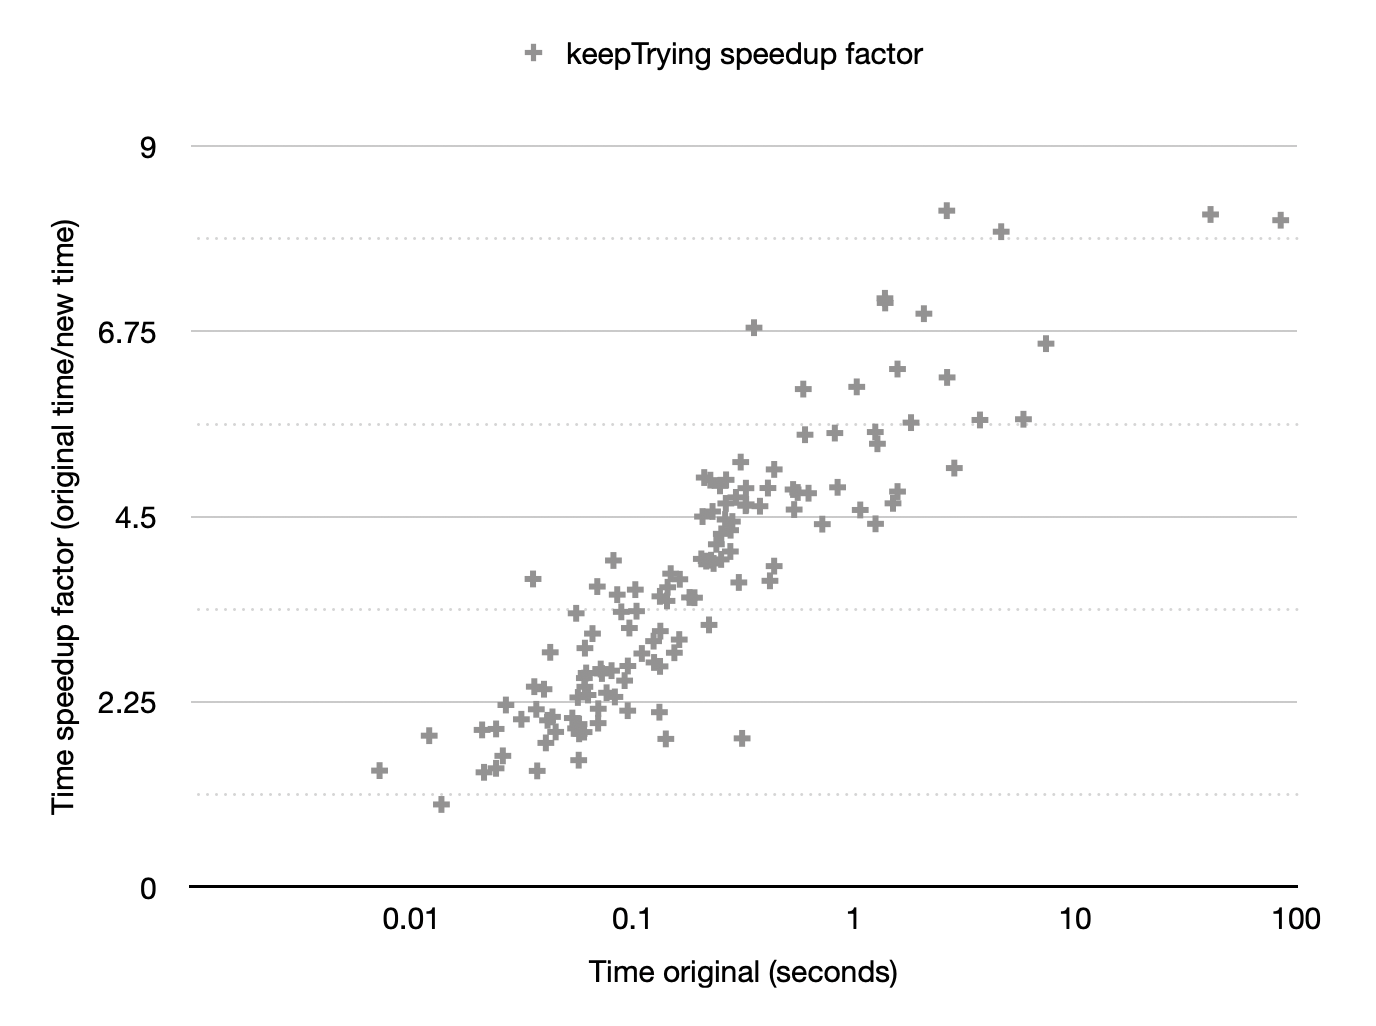
\includegraphics[scale=0.5]{thesis/figure/keepTrying-speedup-factor.png}
    \caption{A plot of the speedup factor for the improved keepTrying algorithm: new time divided by original time, against the original time taken. A linear speedup is the expected result for converting a quadratic algorithm to a linear algorithm.}
    \label{fig:keepTrying-speedup-factor}
\end{figure}

In \autoref{fig:allFunsLocal-speedup-factor} we can see that the allFunsLocal improvement has a speedup factor that is linear on the log-log plot, which indicates that we got an exponential speedup as expected from the theory.

\begin{figure}
    \centering
    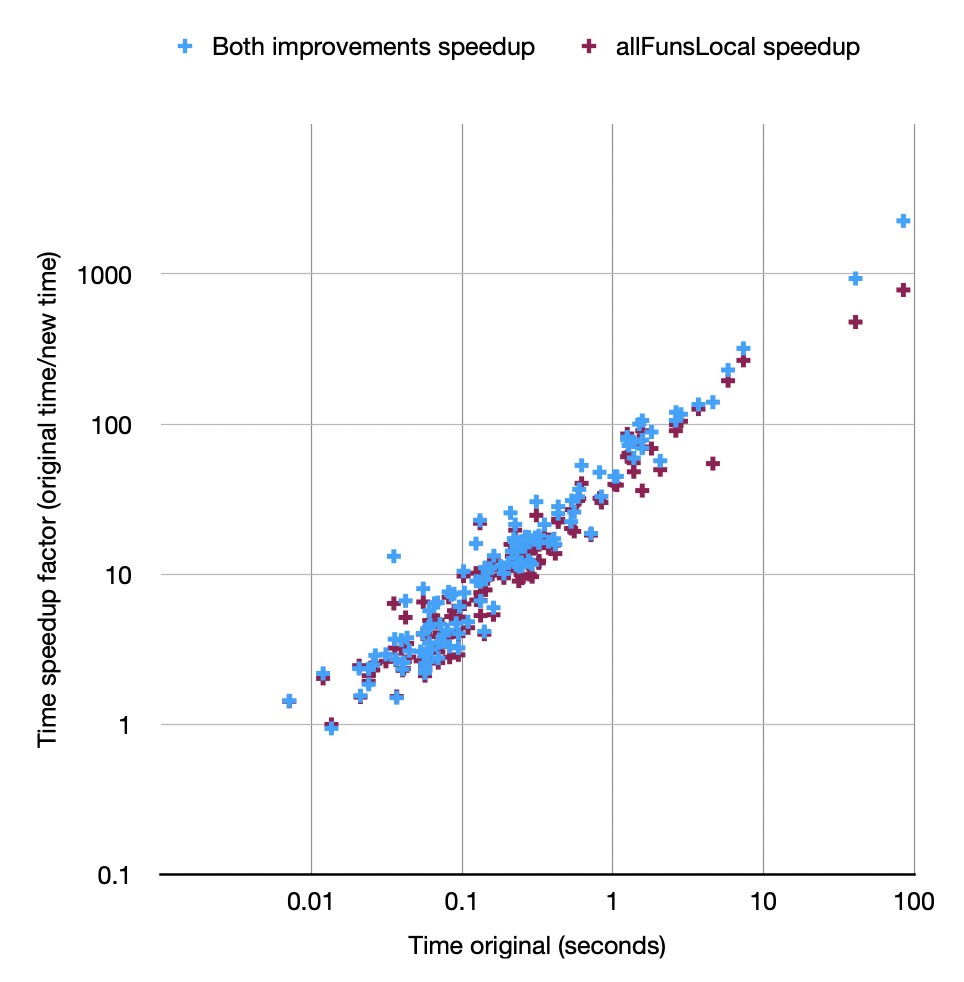
\includegraphics[scale=0.75]{thesis/figure/allFunsLocal-speedup-factor.png}
    \caption{A log-log plot of the speedup factor for the improved allFunsLocal algorithm: new time divided by original time, against the original time taken. The linear pattern indicates an exponential speedup.}
    \label{fig:allFunsLocal-speedup-factor}
\end{figure}

TODO: Write about the minor changes in the resulting trees from the optimized version of the keepTrying function.

% DONE: \todo[inline]{Stacked diagram of all four configurations, with GC time included}


% Running on upto12eng with both improvements and default Garbage Collection settings
% \begin{verbatim}
%    7,783,705,112 bytes allocated in the heap
%   13,905,705,592 bytes copied during GC
%      178,448,096 bytes maximum residency (37 sample(s))
%        2,051,952 bytes maximum slop
%              516 MiB total memory in use (0 MB lost due to fragmentation)
% 
%                                      Tot time (elapsed)  Avg pause  Max pause
%   Gen  0      7351 colls,     0 par    9.128s   9.260s     0.0013s    0.0056s
%   Gen  1        37 colls,     0 par    4.828s   5.069s     0.1370s    0.2165s
% 
%   INIT    time    0.000s  (  0.005s elapsed)
%   MUT     time    2.612s  (  2.666s elapsed)
%   GC      time   13.956s  ( 14.329s elapsed)
%   EXIT    time    0.000s  (  0.005s elapsed)
%   Total   time   16.569s  ( 17.004s elapsed)
% 
%   %GC     time       0.0%  (0.0% elapsed)
% 
%   Alloc rate    2,979,803,301 bytes per MUT second
% 
%   Productivity  15.8% of total user, 15.7% of total elapsed
% \end{verbatim}


\subsection{Garbage Collection time}\label{sect:gc-time}
As can be seen from the previous section, after the improved algorithm is used over 80\% of time is spent on garbage collection. This is in a large part because GHC uses a generational, moving garbage collector\cite{ungar1984generation}, which means that the cost of a garbage collection is proportional to the amount of currently living data \todo{Source for this claim}. In our case we have a large amount of long-living data, which means that every major garbage collection is expensive. The code begins by loading the GF grammar into memory, which for our test grammar takes up around 100 megabytes. There are several ways to mitigate this, but the easiest solution is to tweak the parameters for the garbage collector to make it wait longer before attempting to collect garbage, which reduces the total number of major garbage collections.


% \todo[inline]{The text above should probably go elsewhere (if anywhere at all)}

The tool ghc-gc-tool allows automatically determining which parameters are best for this by running the executable with different parameters and plotting the result. In \autoref{fig:gf-ud-integ-gc-space} we can see the result of running this on the first 60 items of upto12eng.conllu with the ShallowParse grammar from the repository. This number was chosen arbitrarily to make the runtime not be unreasonably long. 

As can be seen in \autoref{fig:GC-time} any initial heap size over 256M drastically reduces the run time and the logs show that the productivity (time spent on non-GC) goes from 15\% to 50\% and that less than one tenth as many garbage collections are performed. This number depends on the size of the GF grammar and it corresponds to the size of the GF grammar after being loaded into memory. Running the command with the default GC parameters shows that the maximum residency is 180M, which is slightly less than the optimal GC parameter value.

\begin{verbatim}
$ ghc-gc-tune -t pdf -spr gf-ud ud2gf grammars/ShallowParse Eng Text
...
gf-ud +RTS -A32768 -H134217728 -RTS ud2gf grammars/ShallowParse Eng Text
    <<GCs 125563, peak   538, resident 177.67m, MUT 1.728s, GC 9.609s>>
gf-ud +RTS -A32768 -H268435456 -RTS ud2gf grammars/ShallowParse Eng Text
    <<GCs   8655, peak   509, resident 176.64m, MUT 1.211s, GC 1.776s>>
...
\end{verbatim}

\begin{figure}
    \centering
    \subcaptionbox{Integral of space use over time\label{fig:GC-time-integ}}
      {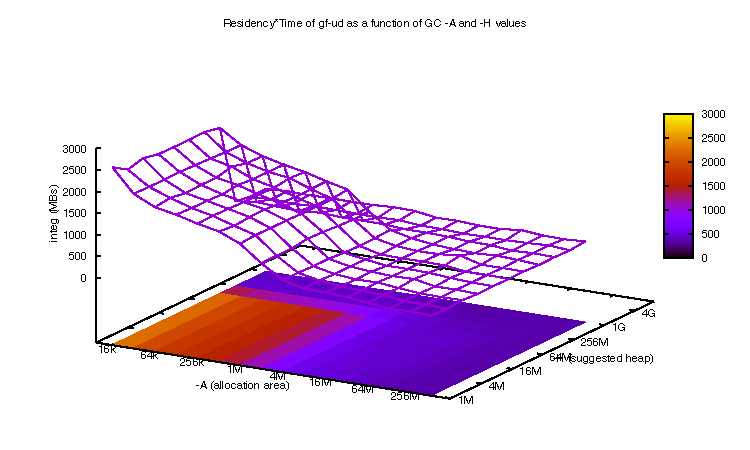
\includegraphics[scale=0.5]{thesis/figure/gf-ud-integ-gc-space.pdf}}
    \subcaptionbox{Time taken\label{fig:GC-time}}
      {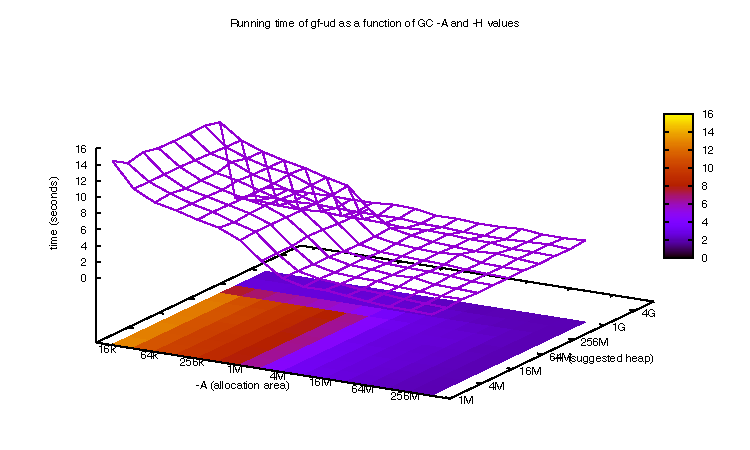
\includegraphics[scale=0.5]{thesis/figure/gf-ud-time-gc-space.pdf}}
    \subcaptionbox{Resident space usage\label{fig:GC-resident-space}}
      {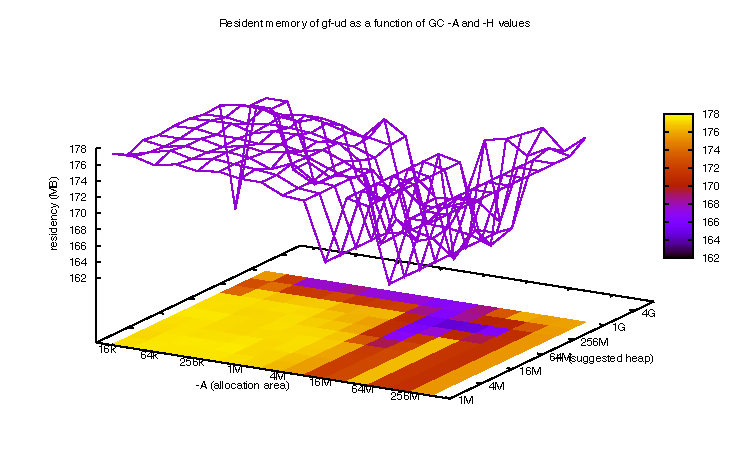
\includegraphics[scale=0.5]{thesis/figure/gf-ud-residency-gc-space.pdf}}
    \subcaptionbox{Peak space usage\label{fig:GC-peak-space}}
      {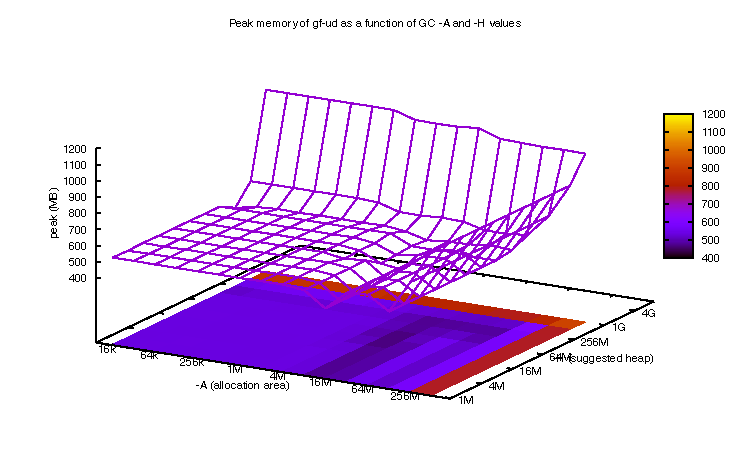
\includegraphics[scale=0.5]{thesis/figure/gf-ud-peak-gc-space.pdf}}
    \caption{The integral of space usage over time for different GC parameters}
    \label{fig:gf-ud-integ-gc-space}
\end{figure}

We also explored other methods for reducing the impact of garbage collection, like compact regions\cite{yang2015efficient}, but they provided no improvement over the simpler method of tweaking the GC parameters and in some cases using them made performance worse, because they force all data stored to be fully evaluated.

\section{Correctness}

Because the accuracy of the conversion depends on manually written annotation files, evaluating the accuracy of the conversion is outside of the scope for this paper.

The optimization of the \texttt{allFunsLocal} function had no impact on the generated trees. However, in some cases the optimization of the \texttt{keepTrying} functions caused different trees to be picked. The different trees are equally valid according to the defined constraints in the annotations and some of them are better and some are worse fits in the example trees we evaluated. See \autoref{sec:multiple_trees} for more details on the multiple possible trees.

\section{Debugging}

The debugging tool that was written in this project allows finding what prevented an \#auxfun macro from being used to convert a tree and anecdotal evidence points towards it being helpful when writing annotations.


\section{Flexibility}

%The new recursive macros made it possible to express the tree shape changes required to convert from the UD way of writing coordination into the GF way of writing conjunctions. Initial tests were successful in converting coordinate structures\footnote{For example ``furry, fluffy and cute'' or ``dog, cat or capybara''} of different lengths and different parts of speech. 

The new recursive macros made it possible to express more significant changes in tree shapes when converting between UD and GF. The motivating example is \emph{coordination}: structures like ``big \emph{or} small'' or ``cats, dogs \emph{and} capybaras''. Before the recursive macros, it was only possible to convert structures with exactly 2 conjuncts, since those had sufficiently similar structure, but now ud2gf can convert coordinate structures of arbitrary length.


\section{Use in robust parsing}

As mentioned in \autoref{sect:background}, the improvement of ud2gf was done as a part of the SMU CCLAW project, with the goal of using ud2gf as a part of a pipeline for parsing unrestricted text in the legal domain.
Experiments on that were performed on a small scale, but the results were deemed unsatisfactory for that specific use. A major part of the problem was the correctness of udpipe itself: legal text contains many uncommon structures, and the initial parses were inaccurate relatively often. 
Given the dissatisfaction with the approach, we never did a quantitative evaluation of the results.

Anecdotally, we found the macro system useful in recovering from parser errors, but it was a lot of tedious work\footnote{Example auxfuns written to recover from errors in udpipe output can be found at \url{https://github.com/smucclaw/sandbox/blob/default/inari/ud/copied-from-dsl/grammars/UDAppEng.labels\#L105-L136}}, with a long tail of fixes that only applied to a single sentence. 

% Write something about the results of using it in the singapore project

% Tie back to section 1.4

% Notes:
% Move info about the singapore project earilier in intro
%



% CONCLUSION
% CREATED BY DAVID FRISK, 2016
\chapter{Conclusion}

You may consider to instead divide this chapter into discussion of the results and a summary. 

\section{Discussion}

\section{Conclusion}


% REFERENCES / BIBLIOGRAPHY
\cleardoublepage
\phantomsection % So hyperref does not link to the section above
\addcontentsline{toc}{chapter}{Bibliography}
\printbibliography

% APPENDICES
\cleardoublepage
\appendix
\setcounter{page}{1}
\pagenumbering{Roman}			% Capitalized roman numbering starting from I (one)

\chapter{Appendix 1: Annotation syntax}


\section{Abstract annotations}

These annotations are associated with an abstract syntax and are in general not specific for a concrete language, but in some cases additional abstract annotations may be needed for a sepecific language.

\subsection{\#cat}

The \lstinline{#cat} annotation describes the mapping from GF categories and UD Part of Speech labels:

\begin{lstlisting}
    #cat GFCategory UD_POS
    #cat N NOUN
\end{lstlisting}

\subsection{\#fun}

The \lstinline{#fun} annotation describes GF functions and which UD dependency label each argument of the function should have (see \autoref{fig:DetCN} for graphical representation of such an annotation). The type signature of the GF function is also required. Each function needs to have at least one head with the label \lstinline{head} and any number of children which are labeled with their corresponding UD dependency labels. It is also possible to add other UD annotations in brackets to a label.

\todo[inline]{How to give this listing a number and a label}
\begin{lstlisting}
    #fun GFFunctionName : FirstArgumentCat -> SecondArgumentCat -> ReturnCat ; first_ud_label second_ud_label
    #fun UseN : N -> CN ; head
    #fun DetCN  : Det -> CN -> NP ; det  head
\end{lstlisting}

The function \lstinline{UseN} only has a single argument (of type \lstinline{N}), so that is required to be the head, while the function \verb|DetCN| has two arguments, of types \verb|Det| and \verb|CN|, the first of which has the dependency label \verb|det|, while the second is the head. An illustration of this can be seen in \autoref{fig:DetCN}.


Both of these annotations are bidirectional and language-independent, since they only refer to the abstract syntax in GF.

\subsection{\#guidelines}

This is only used when checking the validity of an annotation file. The two valid options are \verb|#guidelines UD2| or \verb|#guidelines none|. If the option is omitted, UD2 is assumed. The option UD2 means that only valid ud-labels are allowed, while none means that no such checks are performed.


\section{Evaluation}

\subsection{Recursive \#auxfun macros}

% TODO: This is already in the recursive macros 

In order to improve the ability to create structurally different trees when converting from UD to GF, the ability for macros to be recursive was added. This means that when a macro is substituted, the resulting head is checked again to see if the result is another macro, until no more substitutions are possible. This makes it possible to encode data using Church-encoding, in particular the church encoding for pairs: a higher order function that takes a binary function as an argument and provides the two items it contains to the inner function.

\begin{verbatim}
type Pair a b = forall c. (a -> b -> c) -> c
\end{verbatim}



\hypertarget{annotations-in-gf-ud}{%
\section{Annotations in GF-UD}\label{annotations-in-gf-ud}}

Based on documentation\footnote{https://github.com/GrammaticalFramework/gf-ud/blob/master/doc/annotations.md} written by Aarne Ranta and updated to include new syntax.

Annotations define the relation between GF abstract syntax trees and
dependency trees. There are two kinds of annotations:

\begin{itemize}
% \tightlist
\item
  abstract annotations, which refer only to the abstract syntax
\item
  concrete annotations, which refer also to the concrete syntax
\end{itemize}

Abstract annotations are in principle language-independent. But if we
want to match the conventions of some actual treebank, we may need to
vary them, even in a ``universal'' annotation scheme such as UD.
Concrete annotations are defined for each language separately. But it is
possible to share some of them as well, in particular for languages that
use functors in GF.

To enable maximal sharing of annotations across languages (and other
variations on GF and UD side), annotations can be divided into multiple
files. The \texttt{gfud} program reads these files and builds a data
structure that contains their union. A typical set-up is two files, one
with abstract and one with concrete annotations. An example is
\texttt{grammars/\{Parse.labels,ParseEng.labels,ParseSwe.labels\}},
which are used in combination with \texttt{Parse.pgf} so that
\texttt{Parse.labels} is combined with either \texttt{ParseEng.labels}
or \texttt{ParseSwe.labels}.

The consistency and completeness of annotations can be checked with a
gfud command, for instance:

\begin{verbatim}
$ gfud check-annotations grammars/Parse Eng Utt
\end{verbatim}

(Utt is the start category needed for the checking environment.) When
using annotations and checking their completeness, gfud automatically
adds some rules:

\begin{itemize}
% \tightlist
\item
  \texttt{\#fun\ f\ head} for abstract syntax functions that take just
  one argument
\item
  \texttt{\#morpho\ C\ 0\ \_} for categories whose linearization is just
  a string (or a record with just a string in it)
\end{itemize}

\hypertarget{abstract-annotations}{%
\subsection{Abstract annotations}\label{abstract-annotations}}

\textbf{Function}: \texttt{\#fun}

\begin{verbatim}
   #fun AdvVP  head advmod
\end{verbatim}

There must be a label for each argument. Exactly one argument must have
the label \texttt{head}. If the function has 1 or 0 arguments, the
annotation is not needed. Otherwise, \texttt{gfud} gives a warning about
missing annotations. A generalized form of this is a \textbf{nonlocal
annotation}, such as

\begin{verbatim}
   #fun AdvVP _ PrepNP > head obl
\end{verbatim}

which says that the second argument of \texttt{AdvVP} gets label
\texttt{obl} if it is a tree formed by the function \texttt{PrepNP}.
Nonlocal annotations override normal (local) function annotations. The
above local annotation can be seen as a shorthand of

\begin{verbatim}
   #fun AdvVP _ _ > head advmod
\end{verbatim}

\textbf{Category}: \texttt{\#cat}

\begin{verbatim}
   #cat V2  VERB
\end{verbatim}

Many categories can have the same POS tag. Only those categories that
have lexical items (i.e.~zero-place functions linearized to words) need
this annotation.

Both function and category annotations must be unique in order for
\texttt{gf2ud} to work. However, in the \texttt{ud2gf} direction, two
kinds of deviations may be needed:

\textbf{Annotation guideline}: \texttt{\#guidelines}

\begin{verbatim}
  #guidelines UD2
\end{verbatim}

This flag is used to indicate what guidelines the annotations are
checked against (if any). The default it UD2. It means checking that
each label and POS tag is an actually existing UD2 label or tag. An
alternative is \texttt{none}, meaning that no checks are performed.

\hypertarget{concrete-annotations}{%
\subsection{Concrete annotations}\label{concrete-annotations}}

\textbf{Syncategorematic words}: \texttt{\#word}

\begin{verbatim}
  #word is  be Mood=Ind|Number=Sing|Person=3|Tense=Pres|VerbForm=Fin
\end{verbatim}

These annotations are used for words that appear syncategorematically,
i.e.~elsewhere than as linearizations of zero-place functions. The lemma
should be defined in a \texttt{\#lemma} annotation

\textbf{Syncategorematic lemmas}: \texttt{\#lemma}

\begin{verbatim}
  #lemma UseAP,UseAdv,UseNP be Cop cop head
\end{verbatim}

This means that when any of the functions \texttt{UseAP,\ UseAdv,\ UseN}
introduces the lemma \texttt{be}, it is to be marked with the category
\texttt{Cop} and the label \texttt{cop}. Its head will be the head of
the same construction. Notice that the category is typically an
auxiliary category (see \texttt{\#auxcat} below). A shortcut exists for
saying that a lemma has the same properties in all functions, except
those explicitly defined:

\begin{verbatim}
  #lemma DEFAULT_ be Cop cop head
\end{verbatim}

\textbf{Morphological tags}: \texttt{\#morpho}

\begin{verbatim}
  #morpho V,V2 2 Mood=Ind|Tense=Past|VerbForm=Fin
\end{verbatim}

This annotations tells how the PGF coordinates (numbers) are converted
to morphological tags of UD. The conversion depends on the category,
since different categories have different PGF layouts. To find out what
the coordinates mean, one can use \texttt{gfud\ check-annotations},
which returns examples such as

\begin{verbatim}
  morpho mapping missing:
  #morpho N 1 -- s Sg Gen A-bomb's
  #morpho N 3 -- s Pl Gen A-bombs'
\end{verbatim}

This means that all fields except 1 and 3 have been defined for the
category N. One can also use the text dump of the PGF invoked by the
\texttt{print\_grammar} command of GF:

\begin{verbatim}
  > import ShallowParse.pgf
  > print_grammar
    V := range  [C32 .. C32]
         labels ["s Inf"
                 "s PresSg3"
                 "s Past"
                 "s PastPart"
                 "s PresPart"]
\end{verbatim}

The numbering of labels starts from 0. Thus the third label,
\texttt{s\ Past}, is the one with number 2. Comparing with a UD2
treebank shows that the morphological tag to be used is
\texttt{Mood=Ind\textbar{}Tense=Past\textbar{}VerbForm=Fin}.

\textbf{Discontinuous constituents}: \texttt{\#discont}

\texttt{,head}

\begin{verbatim}
  #discont V2 0-4,head   5,ADV,advmod,head  6,ADP,case,obj
\end{verbatim}

This is applied to discontinuous words, such as V2 with its verb
particle (field 5) and preposition (field 6). The head fields are those
that contain actual verb forms. The other fields need a POS tag, the
word's own label, and the label of the word in the construction that
becomes the head. In this example, the particle (5) is linked to the
head of the construction (i.e.~the verb), whereas the preposition (6) is
linked to the object.

//NB: the target label functionality is currently not implemented, but
all fields are linked to the head.//

\textbf{Multiwords}:
\texttt{\#multiword\ \textless{}category\textgreater{}\ \textless{}head-position\textgreater{}\ \textless{}label\textgreater{}}:

\begin{verbatim}
  #multiword Prep head-first fixed
\end{verbatim}

This annotation tells that, in a multiword preposition, the first word
is the head, and the subsequent words are its dependents with the label
\texttt{fixed}. This follows the guidelines in
https://universaldependencies.org/u/overview/specific-syntax.html;
however, existing treebanks don't seem to follow this strictly. The
guideline example is //in spite of//, where //in// is the \texttt{head}
and the other words are \texttt{fixed}.

//NB: \#multiword works so far only in the gf2ude direction, and
head-last is not supported at all yet//

\textbf{Change of label}:
\texttt{\#change\ \textless{}label\textgreater{}\ \textgreater{}\ \textless{}label\textgreater{}\ \textless{}condition\textgreater{}}:

\begin{verbatim}
  #change obj > obl above case
  #change det > nmod:poss features Poss=Yes|PronType=Prs
\end{verbatim}

These annotations are used at the last step of gf2ud to capture
discrepancies between the grammar and the annotation standard that are
difficult to define in another way. The \texttt{above} condition changes
the label in a node that dominates a certain label. In the example
shown, the \texttt{case} label appears in object that has a preposition,
which is a concrete syntax feature. The \texttt{features} condition
changes the label if the node has certain morphological features. In the
example, possessive pronouns are get the label \texttt{nmod:poss}
instead of the usual \texttt{det}.

\hypertarget{special-concrete-annotations-for-ud2gf}{%
\subsection{Special concrete annotations for
ud2gf}\label{special-concrete-annotations-for-ud2gf}}

The previously shown annotations are used in both directions, gf2ud and
ud2gf. The ud2gf direction uses some additional annotations, listed
here:

\textbf{Alternative function}: \texttt{\#altfun}

\begin{verbatim}
  #altfun ComplV2 head obl
\end{verbatim}

This is needed in \texttt{ud2gf} for reading normal UD, because the
complement of a V2 verb can be labelled either \texttt{obj} of
\texttt{obl} depending on the case governed by the verb.

\textbf{Disabled function}: \texttt{\#disable}

\begin{verbatim}
  #disable UseAP
\end{verbatim}

says that the function \texttt{UseAP} is not to be used in
\texttt{ud2gf}. The reason is that it is overshadowed by a macro
function introducing an auxiliary copula.

\textbf{Auxiliary category}: \texttt{\#auxcat}

\begin{verbatim}
   #auxcat Cop AUX
\end{verbatim}

The category \texttt{Cop} is introduced in the concrete syntax
annotation for the syncategorematic copula verb (see below). In the
\texttt{ud2gf} direction, it is recognized when such a verb, marked by
the POS tag \texttt{AUX}, is encountered in the dependency tree. This is
done by means of auxiliary functions, whose format is somewhat complex,
as they also have to define these extra functions in terms of standard
ones.

\textbf{Auxiliary function}: \texttt{\#auxfun} : = ;

\begin{verbatim}
 #auxfun MkVPS_Perf have vp : Have -> VP -> VPS = MkVPS (TTAnt AAnter TPres) PPos vp ; aux[Tense=Pres] head
\end{verbatim}

The number of argument variables and labels must match the type. The
type can be built from both ordinary and auxiliary categories. As the
definition shows here, the auxiliary category \texttt{Have} argument is
ignored. But the important thing is that - its presence in the UD tree
is recognized, ensuring that all words are taken into account. - it sets
the tense and anteriority of the VPS formed

Auxiliary functions do not necessarily contain auxiliary categories:
they can be just macros collecting the applications of many functions.

\chapter{Conjunction annotation code}\label{appendix:conjunctions}

Below is the complete annotation code for implementing conjunctions for adjective phrases using the recursive macros.

\begin{lstlisting}
-----------------
-- Handling lists
-- This has to be repeated for every category

-- ** Generic, only used inside other macros **
-- Pair_a_b = (a -> b -> r) -> r
#auxfun MkPair_ a b handler : a -> b -> ab2r -> r = handler a b ; head dummy nonexistent
#auxfun UsePair_ handler pair : ab2r -> Pair_a_b -> r = pair handler ; head dummy
-- Triple_a_b_c = (a -> b -> r) -> r
#auxfun MkTriple_ a b c handler : a -> b -> c -> abc2r -> r = handler a b c ; head dummy nonexistent nope
#auxfun UseTriple_ handler triple : abc2r -> Triple_a_b_c -> r = triple handler ; head dummy

-- ** AP **
-- fluffy and cute
#auxfun CommaAP_ ap comma : AP -> Conj -> APComma =  ap ; head punct[LEMMA=\,]

#auxfun AndCuteCont_ and cute : Conj -> AP -> Pair_Conj_AP = MkPair_ and cute ; cc head
-- If we had pattern matching, the above function could have looked like this
-- #auxfun AndCutePatternMatch_ and cute : Conj -> AP -> AP2AP = MkAP2AP and cute ; cc head

#auxfun AP2_ small andCute : AP -> Pair_Conj_AP -> AP = UsePair_ (AP2_helper_ small) andCute ; head conj
#auxfun AP2_helper_ small and cute :  AP -> Conj -> AP -> AP = ConjAP and (BaseAP small cute) ; head dummy nonexistent
-- If we had pattern matching, the above two functions could have been replaced by this
-- #auxfun AP2_ small (MkAP2AP and cute) : AP -> AP2AP -> AP = ConjAP and (BaseAP small cute) ; head conj

#auxfun APBaseComma_ small fluffy andCute : AP -> APComma -> Pair_Conj_AP -> ConjListAP = UsePair_ (APBaseComma_helper_ small fluffy) andCute ; head conj conj
#auxfun APBaseComma_helper_ small fluffy and cute : AP -> APComma -> Conj -> AP -> ConjListAP = MkTriple_ and small (BaseAP fluffy cute) ; head dummy dummy
-- #auxfun APBaseComma_ small fluffy (MkAP2AP and cute)  : AP -> APComma -> AP2AP -> ConjListAP = ConjConsAP and small (BaseAP fluffy cute) ; head conj conj

#auxfun ConjListToAP2_ and_small_furryFluffyCute : ConjListAP -> AP = UseTriple_ ConjListToAP2_helper_ and_small_furryFluffyCute ; head
#auxfun ConjListToAP2_helper_ and small furryFluffyCute : Conj -> AP -> ListAP -> AP = ConjAP and (ConsAP small furryFluffyCute) ; notreal head dummy
-- #auxfun ConjListToAP2_ (ConjConsAP and small furryFluffyCute) : ConjListAP -> AP = ConjAP and (ConsAP small furryFluffyCute) ; head

#auxfun APAddComma_ furry and_small_fluffyCute  : APComma -> ConjListAP -> ConjListAP = UseTriple_ (APAddComma_helper_ furry) and_small_fluffyCute ; conj head
#auxfun APAddComma_helper_ furry and small fluffyCute : APComma -> Conj -> AP -> ListAP -> ConjListAP = MkTriple_ and small (ConsAP furry fluffyCute) ; dummy head
-- #auxfun APAddComma_ furry (ConjConsAP and small fluffyAndCute)  : APComma -> ConjListAP -> ConjListAP = ConjConsAP and small (ConsAP furry fluffyAndCute) ; conj head

\end{lstlisting}

\chapter{Complete benchmark results}\label{appendix:performance}

The benchmark was performed on the branch \texttt{old-benchmark} at
\url{https://github.com/anka-213/gf-ud/tree/old-benchmark}, using the command:

\begin{verbatim}
$ stack bench --ba "--csv results.csv"
\end{verbatim}

Below is a complete table of the results, sorted by time taken for the original algorithm:

\begin{longtable}[]{@{}p{40mm}cccc@{}}
\hline
\thead{Name} & \thead{Original\\algorithm} & \thead{Both\\improvements} & \thead{Fast\\keepTrying} & \thead{Fast\\allFunsLocal} \\
\hline
\endhead
\hline
\endlastfoot
47: Drop the mic . & 7ms & 5ms & 5ms & 5ms \\
45: The dress is contemporary . & 12ms & 5ms & 7ms & 6ms \\
08: Who are they ? & 14ms & 14ms & 14ms & 14ms \\
37: I spotted a few . & 21ms & 9ms & 11ms & 8ms \\
70: Investigation and expeditions to the island continue . & 21ms & 14ms
& 15ms & 14ms \\
32: And what about Australia 's position ? & 24ms & 13ms & 17ms &
12ms \\
17: Then the commercial ends . & 24ms & 10ms & 13ms & 11ms \\
57: Not all transformations in the region have been successful . & 26ms
& 10ms & 16ms & 11ms \\
130: The chalet burned completely down . & 27ms & 9ms & 12ms & 10ms \\
106: The reason for advertising the video in Germany is unclear . & 31ms
& 11ms & 15ms & 12ms \\
97: John of Gaunt died in 1399 . & 35ms & 3ms & 9ms & 6ms \\
129: The ruins were later built over . & 36ms & 10ms & 15ms & 11ms \\
33: Conservationists welcomed the commission 's announcement . & 37ms &
13ms & 17ms & 14ms \\
55: There is no parade and there never has been . & 37ms & 24ms & 26ms &
24ms \\
108: The exchange of Barrosos caused a big stir . & 40ms & 11ms & 16ms &
12ms \\
123: They were primarily on hills . & 40ms & 17ms & 23ms & 18ms \\
50: Is series two working so far ? & 41ms & 16ms & 20ms & 17ms \\
74: Aldrin has been married three times . & 42ms & 6ms & 15ms & 8ms \\
61: Moreover , many of the Macedonian and Persian elite intermarried . &
43ms & 11ms & 21ms & 13ms \\
75: Two measure the lengths of lunar months . & 45ms & 14ms & 24ms &
16ms \\
76: Its importance resides in two facts . & 53ms & 17ms & 26ms & 20ms \\
22: Who can stop this Australia side ? & 55ms & 14ms & 29ms & 14ms \\
112: France does n\textquotesingle t have a good reputation . & 55ms &
7ms & 17ms & 8ms \\
101: Production of the smartphone model was completely discontinued . &
56ms & 19ms & 24ms & 21ms \\
12: That \textquotesingle s what keeps us coming back for more . & 57ms
& 26ms & 37ms & 27ms \\
121: There are different theories about the reasons for leaving the
place . & 57ms & 22ms & 29ms & 23ms \\
118: And what about the parties in what , in historical rights ? & 57ms
& 24ms & 31ms & 25ms \\
67: The study of volcanoes is called volcanology , sometimes spelled
vulcanology . & 60ms & 23ms & 32ms & 23ms \\
15: She was 84 years old . & 60ms & 14ms & 24ms & 16ms \\
24: He 's spoken in favour of torture . & 61ms & 17ms & 25ms & 19ms \\
128: The displaced nuns were moved to the Eibingen cloister . & 61ms &
11ms & 21ms & 12ms \\
114: It will go for assessment . & 61ms & 13ms & 24ms & 14ms \\
56: The Yas Marina Circuit website has exact timings . & 63ms & 20ms &
27ms & 21ms \\
44: They will play on Saturday , 10 June . & 66ms & 10ms & 21ms &
13ms \\
34: Only 50 were marketplaces . & 69ms & 11ms & 19ms & 14ms \\
18: His skill in getting answers for taxpayers will be sorely missed . &
69ms & 25ms & 35ms & 27ms \\
31: Let 's just say he 's wrong . & 70ms & 20ms & 32ms & 23ms \\
81: This city - state emerged in the same period as Sukhothai . & 71ms &
15ms & 27ms & 18ms \\
62: Current land reclamation projects include extending the district of
Fontvieille . & 72ms & 20ms & 28ms & 22ms \\
72: Each poem narrates only a part of the war . & 76ms & 19ms & 32ms &
21ms \\
16: Still , there are questions left unanswered . & 80ms & 19ms & 30ms &
21ms \\
80: Catherine of Russia was also very satisfied . & 81ms & 11ms & 21ms &
12ms \\
119: He believes that nobody waiting for us waits for us . & 83ms & 25ms
& 36ms & 30ms \\
19: More than 330 crew are onboard the ship . & 85ms & 12ms & 24ms &
16ms \\
96: Bouchard suffered a shocking three - set loss . & 88ms & 12ms & 26ms
& 15ms \\
39: A small town with two minarets glides by . & 92ms & 19ms & 37ms &
22ms \\
90: George was appalled by what he saw as their loose morals . & 95ms &
29ms & 44ms & 33ms \\
111: Are workers allowed to keep religious objects on their desks ? &
95ms & 24ms & 35ms & 24ms \\
14: The new iron guidelines mean more donors are needed . & 96ms & 16ms
& 31ms & 19ms \\
20: People got killed there . & 102ms & 10ms & 28ms & 11ms \\
60: The multi-ethnic Achaemenid army possessed many soldiers from the
Balkans . & 104ms & 14ms & 31ms & 16ms \\
105: Do you argue with your alarm clock ? & 110ms & 23ms & 39ms &
25ms \\
59: The 2019 Winter Universiade will be hosted by Krasnoyarsk . & 124ms
& 8ms & 41ms & 12ms \\
94: At least 330,000 people , including 10,000 technicians , were
involved . & 124ms & 14ms & 46ms & 18ms \\
107: The issue might not be over for Barroso . & 132ms & 6ms & 62ms &
6ms \\
13: The current waiting period is eight weeks . & 132ms & 15ms & 37ms &
18ms \\
86: He graduated and obtained an M.A. on 21 April 1882 . & 132ms & 15ms
& 49ms & 20ms \\
88: Only 3000 copies were published of the first edition . & 133ms &
20ms & 43ms & 25ms \\
40: It is his dream to end his career here . & 141ms & 34ms & 78ms &
35ms \\
49: All the medics were armed , except me . & 142ms & 13ms & 41ms &
13ms \\
84: With population growth , new indigenous quarters were created . &
143ms & 16ms & 39ms & 18ms \\
87: He then returned to Kirriemuir . & 148ms & 14ms & 39ms & 16ms \\
27: In this context , railing against trade makes sense . & 154ms & 14ms
& 54ms & 16ms \\
51: I do n\textquotesingle t know why I chose her ... & 162ms & 27ms &
54ms & 30ms \\
115: Durán acts acts as spokesman and Ángel Pintado as treasurer . &
163ms & 12ms & 44ms & 13ms \\
92: Louis Post Dispatch called it one of LaBeouf \textquotesingle s best
performances . & 180ms & 16ms & 51ms & 17ms \\
23: They have one crack at redemption , beating England . & 189ms & 19ms
& 54ms & 20ms \\
77: But the impact of Hispania in the newcomers was also big . & 203ms &
17ms & 51ms & 19ms \\
117: This department now faces new challenges . & 206ms & 17ms & 46ms &
20ms \\
63: In June to August 2010 famine struck the Sahel . & 210ms & 8ms &
42ms & 13ms \\
43: The consumer can boost the demand for change . & 214ms & 15ms & 54ms
& 16ms \\
120: The festive dedication took place on April 30 , 1955 . & 220ms &
13ms & 69ms & 18ms \\
73: This was by boat from continental Europe . & 223ms & 14ms & 45ms &
16ms \\
113: The hit song is " Geronimo " by Sheppard . & 225ms & 11ms & 57ms &
11ms \\
79: Philip next marched against his southern enemies . & 229ms & 20ms &
50ms & 21ms \\
25: I also struggle with passwords . & 231ms & 18ms & 59ms & 21ms \\
109: The good numbers in Asia promptly pushed the stock markets up . &
238ms & 21ms & 57ms & 26ms \\
82: The Army performed well in combat in Cuba . & 247ms & 16ms & 51ms &
20ms \\
09: Not everyone can rise above it . & 250ms & 16ms & 63ms & 17ms \\
99: Von Beust justified the cost increases as lack of detailed planning
. & 251ms & 22ms & 58ms & 27ms \\
66: The Danevirke has remained in German possession ever since . & 261ms
& 17ms & 58ms & 21ms \\
58: She spoke to CNN Style about the experience . & 263ms & 16ms & 56ms
& 19ms \\
21: He worked for the BBC for a decade . & 263ms & 15ms & 53ms & 18ms \\
125: The hymn was well received and the audience demanded an encore . &
275ms & 22ms & 68ms & 23ms \\
93: The car burst into flames , and Kenseth walked away . & 276ms & 16ms
& 64ms & 17ms \\
41: I also wonder whether the Davis Cup played a part . & 281ms & 23ms &
63ms & 28ms \\
83: British cavalry troopers also received excellent mounted
swordsmanship training . & 292ms & 25ms & 62ms & 30ms \\
69: It was declared a wildlife sanctuary in 1975 . & 301ms & 18ms & 81ms
& 20ms \\
03: Maybe the dress code was too stuffy . & 307ms & 17ms & 59ms &
20ms \\
02: \$ 5,000 per person , the maximum allowed . & 311ms & 10ms & 172ms &
13ms \\
68: They generally do not explode catastrophically . & 323ms & 20ms &
70ms & 27ms \\
05: The scheme makes money through sponsorship and advertising . & 324ms
& 18ms & 67ms & 21ms \\
07: Shenzhen \textquotesingle s traffic police have opted for
unconventional penalties before . & 324ms & 20ms & 70ms & 26ms \\
78: Dominican priest Heinrich Kramer was assistant to the Archbishop of
Salzburg . & 352ms & 16ms & 52ms & 19ms \\
38: Back on the train , we continue southwards . & 375ms & 23ms & 81ms &
25ms \\
95: These were almost completely forgotten until after Smith
\textquotesingle s death . & 407ms & 24ms & 84ms & 26ms \\
91: Her 1981 album Wild West was one of her biggest sellers . & 416ms &
26ms & 112ms & 30ms \\
36: Day three , I was back on the EMicro . & 434ms & 17ms & 111ms &
19ms \\
01: The new spending is fueled by Clinton 's large bank account . &
435ms & 15ms & 86ms & 19ms \\
85: Lenny is a persistent bachelor who has poor luck with women . &
529ms & 24ms & 110ms & 26ms \\
71: These plant families are still present in Papua New Guinea . & 535ms
& 17ms & 117ms & 20ms \\
126: I declare the first international Olympic games over . & 555ms &
21ms & 116ms & 29ms \\
29: That 's just legitimately horrendous . & 588ms & 18ms & 97ms &
19ms \\
89: Her latest non-fiction is about Margaret Douglas , Countess of
Lennox . & 599ms & 16ms & 109ms & 19ms \\
53: North Carolina is ground zero in this election . & 621ms & 12ms &
130ms & 15ms \\
10: That \textquotesingle s not what we need in our country , folks . &
717ms & 38ms & 163ms & 39ms \\
122: It contains a monument to Martin Luther King , Jr. & 817ms & 17ms &
148ms & 26ms \\
124: In addition , its process of gilding copper is technologically
noteworthy . & 841ms & 26ms & 173ms & 28ms \\
54: I was just a boy with muddy shoes . & 1s 26ms & 23ms & 169ms &
26ms \\
28: Fast forward to 2016 and this is increasingly worthy of attention .
& 1s 65ms & 24ms & 232ms & 27ms \\
102: On the other hand , Vine was art in six seconds . & 1s 245ms & 16ms
& 225ms & 21ms \\
46: In theory , if done right , it 's un-detectable . & 1s 248ms & 15ms
& 283ms & 15ms \\
65: Like fjords , freshwater lakes are often deep . & 1s 273ms & 18ms &
236ms & 20ms \\
04: It \textquotesingle s like a super power sometimes . & 1s 377ms &
18ms & 192ms & 25ms \\
42: Or is it an expensive standard or prepayment tariff ? & 1s 380ms &
23ms & 194ms & 29ms \\
110: According to the programme , she will speak at 23.45s . & 1s 497ms
& 15ms & 321ms & 19ms \\
100: Simon Krätschmer gropes around alone through the dilapidated ,
sinister barrack . & 1s 569ms & 23ms & 249ms & 44ms \\
30: `` I loved the tropical colours , '' he says . & 1s 570ms & 20ms &
327ms & 22ms \\
127: Today , expansive ruins can be viewed there . & 1s 570ms & 15ms &
327ms & 17ms \\
98: Kühn can only shake his head . & 1s 806ms & 20ms & 320ms & 26ms \\
52: This is a homeland security issue of the most existential kind . &
2s 65ms & 36ms & 297ms & 42ms \\
103: And now he is also world champion . & 2s 621ms & 25ms & 319ms &
29ms \\
48: The result , then , is hardly the cat \textquotesingle s pyjamas . &
2s 630ms & 22ms & 425ms & 27ms \\
116: Its management , however , has n\textquotesingle t been devoid of
criticism . & 2s 835ms & 24ms & 557ms & 27ms \\
11: Our cellphones are so much more than phones these days . & 3s 703ms
& 27ms & 653ms & 29ms \\
06: Previously the jets had only been seen by bloggers . & 4s 619ms &
33ms & 580ms & 85ms \\
35: I do n't call it a beast lightly . & 5s 824ms & 25ms & 1s 25ms &
30ms \\
104: It is now only unclear , in which one . & 7s 365ms & 23ms & 1s
116ms & 28ms \\
26: I can just do that with my life . & 40s 861ms & 44ms & 5s 0ms &
86ms \\
64: In Danish , the word may even apply to shallow lagoons . & 1m 24s
835ms & 38ms & 10s 471ms & 109ms \\
\end{longtable}

% CREATED BY DAVID FRISK, 2016
\chapter{Appendix 2: upto12eng.txt}\label{app:upto12}

Below are the conllu codes for the first few sentences from file \verb|upto12eng.txt| which was used for the benchmarks. The examples comes from the English UD treebank with sentences of at most 12 words.

The complete file can be found at: https://github.com/GrammaticalFramework/gf-ud/blob/master/upto12eng.conllu

\begin{verbatim}
# sent_id = n01002042
# text = The new spending is fueled by Clinton’s large bank account.
1	The	the	DET	DT	Definite=Def|PronType=Art	3	det	3:det	_
2	new	new	ADJ	JJ	Degree=Pos	3	amod	3:amod	_
3	spending	spending	NOUN	NN	Number=Sing	5	nsubj:pass	5:nsubj:pass	_
4	is	be	AUX	VBZ	Mood=Ind|Number=Sing|Person=3|Tense=Pres|VerbForm=Fin	5	aux:pass	5:aux:pass	_
5	fueled	fuel	VERB	VBN	Tense=Past|VerbForm=Part	0	root	0:root	_
6	by	by	ADP	IN	_	11	case	11:case	_
7	Clinton	Clinton	PROPN	NNP	Number=Sing	11	nmod:poss	11:nmod:poss	SpaceAfter=No
8	’s	’s	PART	POS	_	7	case	7:case	_
9	large	large	ADJ	JJ	Degree=Pos	11	amod	11:amod	_
10	bank	bank	NOUN	NN	Number=Sing	11	compound	11:compound	_
11	account	account	NOUN	NN	Number=Sing	5	obl	5:obl:by	SpaceAfter=No
12	.	.	PUNCT	.	_	5	punct	5:punct	_

# newdoc id = n01003
# sent_id = n01003007
# text = $5,000 per person, the maximum allowed.
1	$	$	SYM	$	_	0	root	0:root	SpaceAfter=No
2	5,000	5,000	NUM	CD	NumType=Card	1	nummod	1:nummod	_
3	per	per	ADP	IN	_	4	case	4:case	_
4	person	person	NOUN	NN	Number=Sing	1	nmod	1:nmod:per	SpaceAfter=No
5	,	,	PUNCT	,	_	1	punct	1:punct	_
6	the	the	DET	DT	Definite=Def|PronType=Art	7	det	7:det	_
7	maximum	maximum	NOUN	NN	Number=Sing	1	appos	1:appos	_
8	allowed	allow	VERB	VBN	Tense=Past|VerbForm=Part	7	acl	7:acl	SpaceAfter=No
9	.	.	PUNCT	.	_	1	punct	1:punct	_

# sent_id = n01003013
# text = Maybe the dress code was too stuffy.
1	Maybe	maybe	ADV	RB	_	7	advmod	7:advmod	_
2	the	the	DET	DT	Definite=Def|PronType=Art	4	det	4:det	_
3	dress	dress	NOUN	NN	Number=Sing	4	compound	4:compound	_
4	code	code	NOUN	NN	Number=Sing	7	nsubj	7:nsubj	_
5	was	be	AUX	VBD	Mood=Ind|Number=Sing|Person=3|Tense=Past|VerbForm=Fin	7	cop	7:cop	_
6	too	too	ADV	RB	_	7	advmod	7:advmod	_
7	stuffy	stuffy	ADJ	JJ	Degree=Pos	0	root	0:root	SpaceAfter=No
8	.	.	PUNCT	.	_	7	punct	7:punct	_

\end{verbatim}
And here is the full list of sentences:
\begin{verbatim}
The new spending is fueled by Clinton ’s large bank account .
$ 5,000 per person , the maximum allowed .
Maybe the dress code was too stuffy .
It 's like a super power sometimes .
The scheme makes money through sponsorship and advertising .
Previously the jets had only been seen by bloggers .
Shenzhen 's traffic police have opted for unconventional penalties before .
Who are they ?     
Not everyone can rise above it .
That 's not what we need in our country , folks .
Our cellphones are so much more than phones these days .
That 's what keeps us coming back for more .
The current waiting period is eight weeks .
The new iron guidelines mean more donors are needed .
She was 84 years old .
Still , there are questions left unanswered .
Then the commercial ends .
His skill in getting answers for taxpayers will be sorely missed .
More than 330 crew are onboard the ship .
People got killed there .
He worked for the BBC for a decade .
Who can stop this Australia side ?
They have one crack at redemption , beating England .
He ’s spoken in favour of torture .
I also struggle with passwords .
I can just do that with my life .
In this context , railing against trade makes sense .
Fast forward to 2016 and this is increasingly worthy of attention .
That ’s just legitimately horrendous .
“ I loved the tropical colours , ” he says .
Let ’s just say he ’s wrong .
And what about Australia ’s position ?
Conservationists welcomed the commission ’s announcement .
Only 50 were marketplaces .
I do n’t call it a beast lightly .
Day three , I was back on the EMicro .
I spotted a few .  
Back on the train , we continue southwards .
A small town with two minarets glides by .
It is his dream to end his career here .
I also wonder whether the Davis Cup played a part .
Or is it an expensive standard or prepayment tariff ?
The consumer can boost the demand for change .
They will play on Saturday , 10 June .
The dress is contemporary .
In theory , if done right , it ’s un-detectable .
Drop the mic .     
The result , then , is hardly the cat 's pyjamas .
All the medics were armed , except me .
Is series two working so far ?
I do n't know why I chose her ...
This is a homeland security issue of the most existential kind .
North Carolina is ground zero in this election .
I was just a boy with muddy shoes .
There is no parade and there never has been .
The Yas Marina Circuit website has exact timings .
Not all transformations in the region have been successful .
She spoke to CNN Style about the experience .
The 2019 Winter Universiade will be hosted by Krasnoyarsk .
The multi-ethnic Achaemenid army possessed many soldiers from the Balkans .
Moreover , many of the Macedonian and Persian elite intermarried .
Current land reclamation projects include extending the district of Fontvieille .
In June to August 2010 famine struck the Sahel .
In Danish , the word may even apply to shallow lagoons .
Like fjords , freshwater lakes are often deep .
The Danevirke has remained in German possession ever since .
The study of volcanoes is called volcanology , sometimes spelled vulcanology .
They generally do not explode catastrophically .
It was declared a wildlife sanctuary in 1975 .
Investigation and expeditions to the island continue .
These plant families are still present in Papua New Guinea .
Each poem narrates only a part of the war .
This was by boat from continental Europe .
Aldrin has been married three times .
Two measure the lengths of lunar months .
Its importance resides in two facts .
But the impact of Hispania in the newcomers was also big .
Dominican priest Heinrich Kramer was assistant to the Archbishop of Salzburg .
Philip next marched against his southern enemies .
Catherine of Russia was also very satisfied .
This city - state emerged in the same period as Sukhothai .
The Army performed well in combat in Cuba .
British cavalry troopers also received excellent mounted swordsmanship training .
With population growth , new indigenous quarters were created .
Lenny is a persistent bachelor who has poor luck with women .
He graduated and obtained an M.A. on 21 April 1882 .
He then returned to Kirriemuir .
Only 3000 copies were published of the first edition .
Her latest non-fiction is about Margaret Douglas , Countess of Lennox .
George was appalled by what he saw as their loose morals .
Her 1981 album Wild West was one of her biggest sellers .
Louis Post Dispatch called it one of LaBeouf 's best performances .
The car burst into flames , and Kenseth walked away .
At least 330,000 people , including 10,000 technicians , were involved .
These were almost completely forgotten until after Smith 's death .
Bouchard suffered a shocking three - set loss .
John of Gaunt died in 1399 .
Kühn can only shake his head .
Von Beust justified the cost increases as lack of detailed planning .
Simon Krätschmer gropes around alone through the dilapidated , sinister barrack .
Production of the smartphone model was completely discontinued .
On the other hand , Vine was art in six seconds .
And now he is also world champion .
It is now only unclear , in which one .
Do you argue with your alarm clock ?
The reason for advertising the video in Germany is unclear .
The issue might not be over for Barroso .
The exchange of Barrosos caused a big stir .
The good numbers in Asia promptly pushed the stock markets up .
According to the programme , she will speak at 23.45 .
Are workers allowed to keep religious objects on their desks ?
France does n't have a good reputation .
The hit song is " Geronimo " by Sheppard .
It will go for assessment .
Durán acts acts as spokesman and Ángel Pintado as treasurer .
Its management , however , has n't been devoid of criticism .
This department now faces new challenges .
And what about the parties in what , in historical rights ?
He believes that nobody waiting for us waits for us .
The festive dedication took place on April 30 , 1955 .
There are different theories about the reasons for leaving the place .
It contains a monument to Martin Luther King , Jr.
They were primarily on hills .
In addition , its process of gilding copper is technologically noteworthy .
The hymn was well received and the audience demanded an encore .
I declare the first international Olympic games over .
Today , expansive ruins can be viewed there .
The displaced nuns were moved to the Eibingen cloister .
The ruins were later built over .
The chalet burned completely down .
\end{verbatim}


\end{document}
